% Options for packages loaded elsewhere
\PassOptionsToPackage{unicode}{hyperref}
\PassOptionsToPackage{hyphens}{url}
% !TeX program = pdfLaTeX
\documentclass[12pt]{article}
\usepackage{amsmath}
\usepackage{graphicx,psfrag,epsf}
\usepackage{enumerate}
\usepackage{textcomp}


%\pdfminorversion=4
% NOTE: To produce blinded version, replace "0" with "1" below.
\newcommand{\blind}{0}

% DON'T change margins - should be 1 inch all around.
\addtolength{\oddsidemargin}{-.5in}%
\addtolength{\evensidemargin}{-1in}%
\addtolength{\textwidth}{1in}%
\addtolength{\textheight}{1.7in}%
\addtolength{\topmargin}{-1in}%

%% load any required packages here



% tightlist command for lists without linebreak
\providecommand{\tightlist}{%
  \setlength{\itemsep}{0pt}\setlength{\parskip}{0pt}}

% From pandoc table feature
\usepackage{longtable,booktabs,array}
\usepackage{calc} % for calculating minipage widths
% Correct order of tables after \paragraph or \subparagraph
\usepackage{etoolbox}
\makeatletter
\patchcmd\longtable{\par}{\if@noskipsec\mbox{}\fi\par}{}{}
\makeatother
% Allow footnotes in longtable head/foot
\IfFileExists{footnotehyper.sty}{\usepackage{footnotehyper}}{\usepackage{footnote}}
\makesavenoteenv{longtable}

% Pandoc citation processing
\newlength{\cslhangindent}
\setlength{\cslhangindent}{1.5em}
\newlength{\csllabelwidth}
\setlength{\csllabelwidth}{3em}
\newlength{\cslentryspacingunit} % times entry-spacing
\setlength{\cslentryspacingunit}{\parskip}
% for Pandoc 2.8 to 2.10.1
\newenvironment{cslreferences}%
  {}%
  {\par}
% For Pandoc 2.11+
\newenvironment{CSLReferences}[2] % #1 hanging-ident, #2 entry spacing
 {% don't indent paragraphs
  \setlength{\parindent}{0pt}
  % turn on hanging indent if param 1 is 1
  \ifodd #1
  \let\oldpar\par
  \def\par{\hangindent=\cslhangindent\oldpar}
  \fi
  % set entry spacing
  \setlength{\parskip}{#2\cslentryspacingunit}
 }%
 {}
\usepackage{calc}
\newcommand{\CSLBlock}[1]{#1\hfill\break}
\newcommand{\CSLLeftMargin}[1]{\parbox[t]{\csllabelwidth}{#1}}
\newcommand{\CSLRightInline}[1]{\parbox[t]{\linewidth - \csllabelwidth}{#1}\break}
\newcommand{\CSLIndent}[1]{\hspace{\cslhangindent}#1}

\usepackage{amsmath}
\usepackage{subfig}

\IfFileExists{bookmark.sty}{\usepackage{bookmark}}{\usepackage{hyperref}}
\IfFileExists{xurl.sty}{\usepackage{xurl}}{} % add URL line breaks if available
\hypersetup{
  pdftitle={Bayesian Detection of Bias in Peremptory Challenges Using Historical Strike Data},
  pdfkeywords={Batson challenge, peremptory strikes, power prior, Bayesian},
  hidelinks,
  pdfcreator={LaTeX via pandoc}}



\begin{document}


\def\spacingset#1{\renewcommand{\baselinestretch}%
{#1}\small\normalsize} \spacingset{1}


%%%%%%%%%%%%%%%%%%%%%%%%%%%%%%%%%%%%%%%%%%%%%%%%%%%%%%%%%%%%%%%%%%%%%%%%%%%%%%

\if0\blind
{
  \title{\bf Bayesian Detection of Bias in Peremptory Challenges Using Historical Strike Data}

  \author{
        \href{https://orcid.org/0000-0001-7387-1307}{Sachin S. Pandya} \\
    University of Connecticut\\
     and \\     Xiaomeng Li \\
    University of Connecticut\\
     and \\     \href{https://orcid.org/0000-0003-1934-1932}{Eric Barón} \\
    University of Connecticut\\
     and \\     \href{https://orcid.org/0000-0002-9576-0517}{Timothy E. Moore} \\
    University of Connecticut\\
      }
  \maketitle
} \fi

\if1\blind
{
  \bigskip
  \bigskip
  \bigskip
  \begin{center}
    {\LARGE\bf Bayesian Detection of Bias in Peremptory Challenges Using Historical Strike Data}
  \end{center}
  \medskip
} \fi

\bigskip
\begin{abstract}
United States law bars using peremptory strikes during jury selection because of prospective juror race, ethnicity, sex, or membership in certain other cognizable classes. Here, we extend a Bayesian approach for detecting such illegal strike bias by showing how to incorporate historical data on an attorney's use of peremptory strikes in past cases. In so doing, we use the power prior to adjust the weight of such historical information in the analysis. Using simulations, we show how the choice of the power prior's discounting parameter influences bias detection (how likely the credible interval for the bias parameter excludes zero), depending on the degree of incompatibility between current and historical trial data. Finally, we extend this approach with a prototype software application that lawyers could use to detect strike bias in real time during jury-selection. We illustrate this application's use with real historical strike data from a convenience sample of cases from one court.
\end{abstract}

\noindent%
{\it Keywords:} Batson challenge, peremptory strikes, power prior, Bayesian

\vfill

\newpage
\spacingset{1.9} % DON'T change the spacing!

\hypertarget{introduction}{%
\section{Introduction}\label{introduction}}

In the United States, individuals selected for jury service appear in court as scheduled and are questioned by the parties' attorneys and the trial judge. During this process, a prospective juror, if not excused by the trial judge for cause, may still be dismissed if a party's attorney uses one of their limited number of peremptory challenges against them. By asserting a peremptory challenge, a party can declare a prospective juror ineligible (``strikes'' that juror) for a seat on the jury without the burden of explaining why.

Since \emph{Batson v. Kentucky} (1986), a party violates the Equal Protection Clause of the United States Constitution by using peremptory challenges if motivated by the prospective jurors' race, ethnicity, sex, or certain other cognizable classes. The party bringing a \emph{Batson} challenge bears the burden of proving such illegal bias is more likely than not to be true (LaFave et al. 2022, \(\S\) 22.3(d)).

A \emph{Batson} challenge typically proceeds in a four-step sequence. First, the attorney must decide whether to challenge the opposing attorney's use of one or more peremptory strikes as based on illegal bias. Second, if challenged, the challenger must meet an initial burden (the \emph{prima facie} case) of producing just enough evidence of strike bias to raise a sufficient initial inference of illegal bias. Third, the striking attorney must proffer permissible reasons for their challenged strikes. Fourth, the challenger must discredit those proffered reasons and ultimately persuade the trial judge that it is more likely than not that the striking attorney acted with illegal bias.

For similar challenges under State law, a few States require only that an ``objective observer'' or an ``objectively reasonable person'' would find that race, ethnicity or another cognizable-class was a ``factor'' in that party's use of strikes (Wash. General Rule 37(e); Calif. Code of Civil Procedure \(\S\) 231.7(d)(1); Conn. Superior Court Rule 5-12(d)). Peremptory-challenge procedure, and thus the task of proving such illegal bias, varies not only by State, but also by court, including the number of peremptory challenges assigned to each side and the order in which each party uses those strikes (Williams 2017).

In any case, evidence of such illegal bias may include data on the use of peremptory challenges in past cases (\emph{Flowers v. Mississippi} (2019), p.~2243; Wash. General Rule 37(g)(v); Calif. Code Civil Procedure \(\S\) 231.7(d)(3)(G)). Prior studies have collected such historical strike data in past cases and reported the observed difference in strike rates by race or sex. Typically, they test for the probability of observing a non-zero difference in strike rates by the race or sex of the struck prospective jurors, given repeated sampling from a hypothetical population of peremptory strikes with zero such difference (e.g., Eisenberg 2017; Grosso and O'Brien 2012; for discussion, see Gastwirth and Xu 2014, 289--97; Gastwirth and Yu 2013). Prior studies have also modeled how much a prospective juror's race affected the odds of being struck. For different modeling approaches using the same historical strike data from Mississippi, see Craft (2018); DeCamp (2021); and Dunn and Zhuo (2022).

Without historical strike data, there is a higher risk of underpowered and inflated estimates of attorney strike bias, because of the low number of strikes per trial: typically from 6 to 15 strikes per party, depending on the jurisdiction (National Center for State Courts: Center for Jury Studies 2018). Yet, complete pooling of current and historical strike data may be affected by the degree of incompatibility between current and historical strike data. Such incompatibility may occur if missing historical strike is missing not at random due to incomplete or inaccessible jury-selection records (Grosso and O'Brien 2017; Wright, Chavis, and Parks 2018).

Incompatibility may also occur if attorney strike bias depends on certain trial-level characteristics (e.g., defendant race, charge severity) that take on one value in the current trial but that vary across the historical trials. For example, suppose an attorney who is more likely to strike Black prospective jurors because the defendant is Black; who has zero strike bias in cases with white defendants; and whose historical strike data comes from past trials with an equal number of Black and white defendants. If so, then inferring strike bias in the current trial with a Black defendant may depend in part on whether we use all the historical data or only the subset of past trials with Black defendants.

As a result, for any given estimate of strike bias in a current trial, incompatibility between strike data from that current trial and strike data from past trials can lead to inflated type I error and reduced power (Bennett et al. 2021). Other methods to increase power may in turn require adjusting for incompatibility implicitly. For example, Gastwirth and Xu (2014, 295--97) stratify strike data by trial and apply the Cochran-Mantel-Haenszel test, albeit after first selecting only historical strike data from past trials that are ``similar'' in their bias-salient characteristics to the current trial {[}p.~289, 297{]}. This initial step presumably aims to reduce incompatibility due to variation in those salient characteristics. Any such choice of ``similar'' historical strike data would need to be disclosed and justified.

In this paper, we extend a Bayesian approach to \emph{Batson} and similar challenges (Kadane 2021, 2018b, 2018a) to incorporate historical strike data in a manner that allows for transparently adjusting for the assumed degree of incompatibility between current and historical trials. We proceed in three steps. First, we specify a model of the peremptory-strike process in the court of interest that includes a bias parameter to which we assign an initial prior distribution. Second, we use an attorney's strike data from past trials, generated by that same peremptory-strike process, to estimate a posterior distribution for that bias parameter. In so doing, we use the power prior (Chen and Ibrahim 2000; Ibrahim et al. 2015; for a gentle introduction, see Viele et al. 2014). The power prior raises the likelihood of the historical strike data to a fixed power (\(\alpha\)), typically between zero and one, to down-weight the historical strike data in accord with expected incompatibility between the historical trials and the current trial. Zero denotes no weight to the historical data (for complete incompatibility) and one denotes equal weight (for complete compatibility). Third, we use this posterior distribution as an informative prior for the bias parameter in the current trial.

We demonstrate this approach with simulations in which we vary the degree of incompatibility between current and historical trial data, and test how well we can ``detect'' attorney strike bias, i.e., whether the credible interval for the bias parameter excludes zero, given different values of the power prior's alpha parameter. Then, we present a software prototype that encodes the same approach with actual historical strike data from a convenience sample of criminal cases from one court. With that data, we use the prototype to illustrate how attorneys and others can use this approach to detect strike bias in real time during jury selection.

\begin{figure}[h]

{\centering 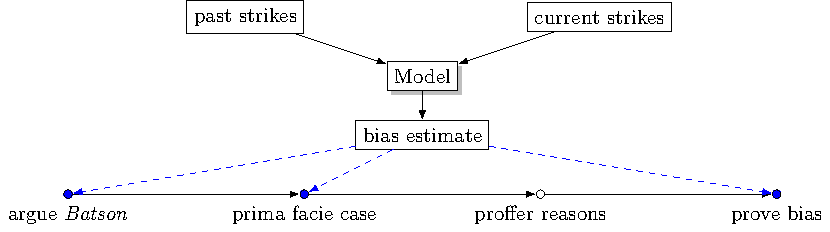
\includegraphics[width=1\linewidth]{../figures/batson_workflow_fig2} 

}

\caption{Inference from Historical Strike Data at Key Steps of Batson Challenge. Filled circles indicate steps for which bias estimates could be used.}\label{fig:batsonworkflowfig}
\end{figure}

To be sure, neither this nor any other statistical approach can automatically detect \emph{Batson} violations, because \emph{Batson} law permits any evidence of strike bias, not just strikes in past cases. And \emph{Batson} law requires the trial judge to weigh all such evidence to decide whether strike bias likely exists (the \emph{Batson} violation). Still, \emph{before} accounting for other relevant evidence of strike bias, our approach can help attorneys detect strike bias, given current and historical strike data, a valid model of the relevant court's strike procedure, and a fixed value for the power prior's \(\alpha\) parameter. After testing for sensitivity of bias detection to different fixed \(\alpha\) values for the power prior (Carvalho and Ibrahim 2021, 5252; Ibrahim et al. 2015, 3734), attorneys can then combine the resulting inference with other evidence to decide whether to argue \emph{Batson}; to prove the \emph{Batson} prima facie case; and to persuade the trial judge to find a \emph{Batson} violation (Figure \ref{fig:batsonworkflowfig}).

\hypertarget{methods}{%
\section{Methods}\label{methods}}

\hypertarget{statistical-procedure}{%
\subsection{Statistical Procedure}\label{statistical-procedure}}

Following others (e.g., Kadane 2018b; Barrett 2007; Gastwirth 2005, 183), we model a peremptory-challenge process in which each party strikes prospective jurors in an alternating sequence. Under such a procedure, the trial judge rules on all challenges for cause before the parties exercise any peremptory strikes. Then, of the potential jurors who remain, a subset of them are subject to peremptory strike, usually a number that corresponds to the number seats on the jury (plus alternates, if any). The parties exercise their strikes on anyone among this subset of potential jurors in an alternating sequence. Once all strikes are used or waived, the remaining prospective jurors are each assigned to seats on the jury plus a few alternate jurors.

Accordingly, for any given case \(i\) in which jury selection occurs, let \(j\) denote a peremptory strike used, and let \(\delta_{ij}\) denote whether or not a party used that strike on a person who belongs to a ``cognizable class''. If ``race'' is the bias type of interest, the cognizable class is racial minority jurors (\(\delta_{ij} =1\), 0 for White jurors). If ``sex'' is the bias of interest, the cognizable class is female jurors (\(\delta_{ij} = 1\), 0 for male jurors). In turn, let \(c_{ij}\) denote the number of cognizable class members subject to strike; and \(m_{ij}\) denote the number of cognizable class non-members subject to strike, such that \(c_{ij}+m_{ij}\) is the total number of jurors potentially subject to strike. If there is no bias, the probability is \(\frac{c_{ij}}{c_{ij}+m_{ij}}\) for striking a cognizable class member, and \(1-\frac{c_{ij}}{c_{ij}+m_{ij}}\) for striking someone who does not belong to that class.

By adding one parameter \(w\), we can measure \emph{bias} by different values of \(w\) by defining the probability of a cognizable class member being struck to be \(\frac{wc_{ij}}{wc_{ij}+m_{ij}}\). To avoid making the weight of the non-cognizable class be the reciprocal of the weight of cognizable class, let \(b = log(w)\).

Accordingly, for any given value of the bias parameter \(b\), the probability of strike of a member from either class, or \(Pr(\delta_{ij})\), is such that:

\begin{equation}
Pr(\delta_{ij} | b) = 
\begin{cases}
  \frac{(e^b)c_{ij}}{(e^b)c_{ij}+m_{ij}} & \text{for }\delta_{ij}=1\\    
  \frac{m_{ij}}{(e^b)c_{ij}+m_{ij}} & \text{for }\delta_{ij}=0  \label{eq:model1}
\end{cases} 
\end{equation} This Equation \eqref{eq:model1} is equivalent to

\begin{equation}
Pr(\delta_{ij}| b) = \left(\frac{(e^b)c_{ij}}{(e^b)c_{ij}+m_{ij}}\right)^{\delta_{ij}} \left(\frac{m_{ij}}{(e^b)c_{ij}+m_{ij}}\right)^{1-\delta_{ij}}
\label{eq:model2}
\end{equation}

Given the strike data we have, i.e., \(\delta_{ij}\), \(c_{ij}\), and \(m_{ij}\), by estimating the value of \(b\), we can measure bias when a party is striking potential jurors. If \(b = 0\), there is no bias, and the probability of strike is simply a function of the share of cognizable members (non-members) in the pool of prospective jurors that could be struck. If \(b>0\), we infer that the the party has bias favoring a strike against a juror falling within the cognizable class (e.g., the juror is a racial minority). Where \(b<0\), the party has a preference for a juror within the cognizable class.

The likelihood function of \(b\) is

\begin{equation}  
L(b|\delta) = \prod_{i=1}^{n_i} \prod_{j=1}^{n_j}\left(\frac{(e^b)c_{ij}}{(e^b)c_{ij}+m_{ij}}\right)^{\delta_{ij}} \left(\frac{m_{ij}}{(e^b)c_{ij}+m_{ij}}\right)^{1-\delta_{ij}}
\label{eq:model3}
\end{equation} where \(n_{i}\) is the total number of jury selections (trials), \(n_j\) is the total number of peremptory strikes, and \(\delta=(\delta_{11},\delta_{12},\dots,\delta_{{n_i}{n_j}})\)

\hypertarget{incorporating-historical-strike-data}{%
\subsection{Incorporating historical strike data}\label{incorporating-historical-strike-data}}

We incorporate data on strikes in past cases and allow for adjustment of the weight of that historical strike data on the posterior distribution of the bias parameter. To do this, we introduce the power prior:

\begin{equation}  
\pi(b|\delta_0,\alpha_0) \propto L(b|\delta_0)^{\alpha_0}\pi_0(b)
\label{eq:powerprior}
\end{equation} where \(0 \le \alpha_0 \le 1\) is the parameter controlling the weight of the historical information; \(\delta_0=(\delta_{011},\delta_{012},\dots,\delta_{0{n_i}{n_j}})\) is the observed historical data; \(L(b|\delta_0)\) is the likelihood function of \(b\) given the historical data; and \(\pi_0(b)\) is the initial prior before the historical data is observed.

In this paper, we assume that the law for \emph{Batson} and similar challenges entails a weakly-informative initial prior:

\begin{equation}  
\pi_0(b) \sim Normal(\mu = 0, \sigma = 2)
\label{eq:initialprior}
\end{equation}

For this initial prior, we let \(\mu = 0\), because the law assigns the burden of proof in a \emph{Batson} challenge to the party bringing the challenge. Thus, if the challenging party produces no relevant evidence of illegal bias, the law requires a trial judge to reject the challenge as unproven. This is tantamount to treating zero as the most-likely value of the bias parameter, absent any data. Moreover, we take the law to imply that, absent any data, one must assume that higher degrees of illegal bias are less likely than lower degrees of bias. For this reason, we use a normal (Gaussian) distribution with \(\sigma = 2\). This prior accords with Kadane (2021, 51), who suggests a prior for estimating \emph{Batson} strike bias that is at least unimodal, symmetric, and not dependent on the data.

After including the historical information through the power prior, the posterior distribution of \(b\) is proportional to the product of likelihood function of \(b\) and the power prior of \(b\) is

\begin{equation}
 \pi(b|\delta,\delta_0) \propto L(b|\delta)L(b|\delta_0)^{\alpha_0}\exp\left(-\frac{(b-\mu)^2}{2\sigma^2}\right)
  \label{eq:model4}
\end{equation} where

\begin{equation}
L(b|\delta_0) = \prod_{i=1}^{n_{0i}} \prod_{j=1}^{n_{0j}}\left(\frac{(e^b)c_{0ij}}{(e^b)c_{0ij}+m_{0ij}}\right)^{\delta_{0ij}} \left(\frac{m_{0ij}}{(e^b)c_{0ij}+m_{0ij}}\right)^{1-\delta_{0ij}}
\label{eq:model5}
\end{equation} is the likelihood function of \(b\) given historical data; \(n_{0i}\) is the total number of jury selections (trials) in the historical data; \(n_{0j}\) is the total number of peremptory strikes in the historical data; and \(\delta_{0ij}\) denotes whether or not a party used that strike on a person who belongs to a cognizable class in the historical trials.

\hypertarget{simulation-results}{%
\subsection{Model Performance on Simulated Data}\label{simulation-results}}

To evaluate the proposed method, we conducted a simulation study using Stan 2.261, a Hamiltonian Monte Carlo engine for Bayesian inference by way of R version 4.2.2 and RStan and RStan (Stan Development Team 2022). These simulations primarily show how much the size of the historical data affects our ability to detect bias and how much the power prior discounted the weight of the historical data. As introduced above, \(b > 0\) represents a prosecutor's bias against a prospective juror within the cognizable class, while \(b = 0\) denotes no bias. For simplicity, we assume the defense attorney has no bias.

Because we use the power prior, we can control how much we account for the historical strike data by modifying the discounting parameter \(\alpha\) (denoted as \(\alpha_0\) in Equations \eqref{eq:powerprior} and \eqref{eq:model4}). If \(\alpha=1\), the historical strike data is equally weighted with the data on strikes in the current trial. If \(\alpha<1\), the historical data are discounted and weighted proportionally less than the current trial data. We assign \(\alpha<1\) to evaluate how sensitive the posterior of the bias parameter is to the historical data on strikes. Accordingly, in the simulation study, we evaluated different values of \(\alpha\): \(\alpha=\{0,0.1,0.2,0.3,0.4,0.5,0.6,0.7,0.8,0.9,1\}\) to show how that parameter affected bias detection.

We generated historical strike data of three sizes (same, double, and triple the size of current data, i.e., data on one, two, or three previous trials) using seven different values of the bias parameter for generating that historical data \(b_{hist}=\{0,0.5,1,1.5,2, 2.5,3\}\).

To generate data, we generated strike data for a current trial using seven different values of the bias parameter \(b_{curr}=\{0,0.5,1,1.5,2, 2.5,3\}\). To evaluate the strength of the power prior as a function of the degree of incompatibility between current and historical strike data (\(\lvert b_{curr} - b_{hist} \rvert > 0\)), we assigned \(b_{hist}\) the same bias values as \(b_{curr}\), i.e., \(b_{hist}=\{0,0.5,1,1.5,2, 2.5,3\}\). We did this to simulate noise in the historical strike data that can arise due to not-at-random missingness or because a confounder (e.g.~defendant race, charge severity) affects \(b_{curr}\) but not of all the past trials in the historical strike data.

For our simulation, we define bias detection as the proportion of times we identify bias when bias is present in the current trial, i.e., \(b_{curr} > 0\) , based on whether credible intervals of the bias parameter exclude zero. Since we use a weakly-informative prior that pulls the estimate of \(b_{curr}\) towards zero, we focus on how accurately our model can detect that bias, \emph{not} on how accurately the model can recover the true value of \(b_{curr}\) (i.e., a traditional coverage rate). For instance, a 90\% bias detection rate means that in 900 of 1000 model fits, a given credible interval does not contain zero if the \(b_{curr}\) is not zero. Put another way, if we set \(b_{curr}>0\), we calculate the proportion of the 95\% credible intervals that lie to the right of zero (lower bound is positive) among the 1000 model fits. For each scenario, we generated 1000 data sets and fit the model on those data sets. For each replicate, we generated a HMC sample of 10,000 iterations with a burn-in period of 1000 iterations. For each replicate, we calculated the posterior mean and \(80\%\), \(90\%\), and \(95\%\) highest posterior density intervals for \(b_{curr}\).

Additionally, we present sensitivity analysis for the number of available strikes per trial (6 strikes, 10 strikes, and 15 strikes for each attorney). Thus, in total, we considered 4851 different scenarios, i.e.~the combination of 7 different bias parameters of current data and of historical data, 3 different amounts of historical data, 11 different values for the power prior weight parameter, and for 3 combinations of the total number of strikes.

\hypertarget{results}{%
\section{Results}\label{results}}

Figure \ref{fig:figbd9515} depicts the bias detection rate with an 95\% credible interval for the 15 strikes scenario. When \(b_{curr}\) is high (close to 3), the bias detection rate is high (very close to 1). However, when \(b_{curr}\) is lower (close to zero), the bias detection rate drops below 0.8. When there is no bias in the current or historical trials (\(b_{curr} = b_{hist} = 0\)), the bias detection rate for the 95\% credible interval is 0.05 or less. As we place more weight on the historical strike data (as \(\alpha\) increases), and the historical strike data is consistent with current information (high compatibility), the bias detection rate is close to 1, especially when bias is high (upper right-hand corner of plots). Conversely, as \(\alpha\) decreases, bias detection is only high when there is high bias in the current trial (\(b_{curr} \geq 1.5\)). Increasing the number of historical trials leads to an increase in bias detection especially when current and historical trials are compatible. However, when current and historical trials are incompatible, both type I and type II error can be high if \(\alpha\) is close to one. As we discuss in section \ref{selectingalpha} below, the choice of \(\alpha\) depends on assumptions about the degree of incompatibility of current and historical trials.

\begin{figure}

{\centering 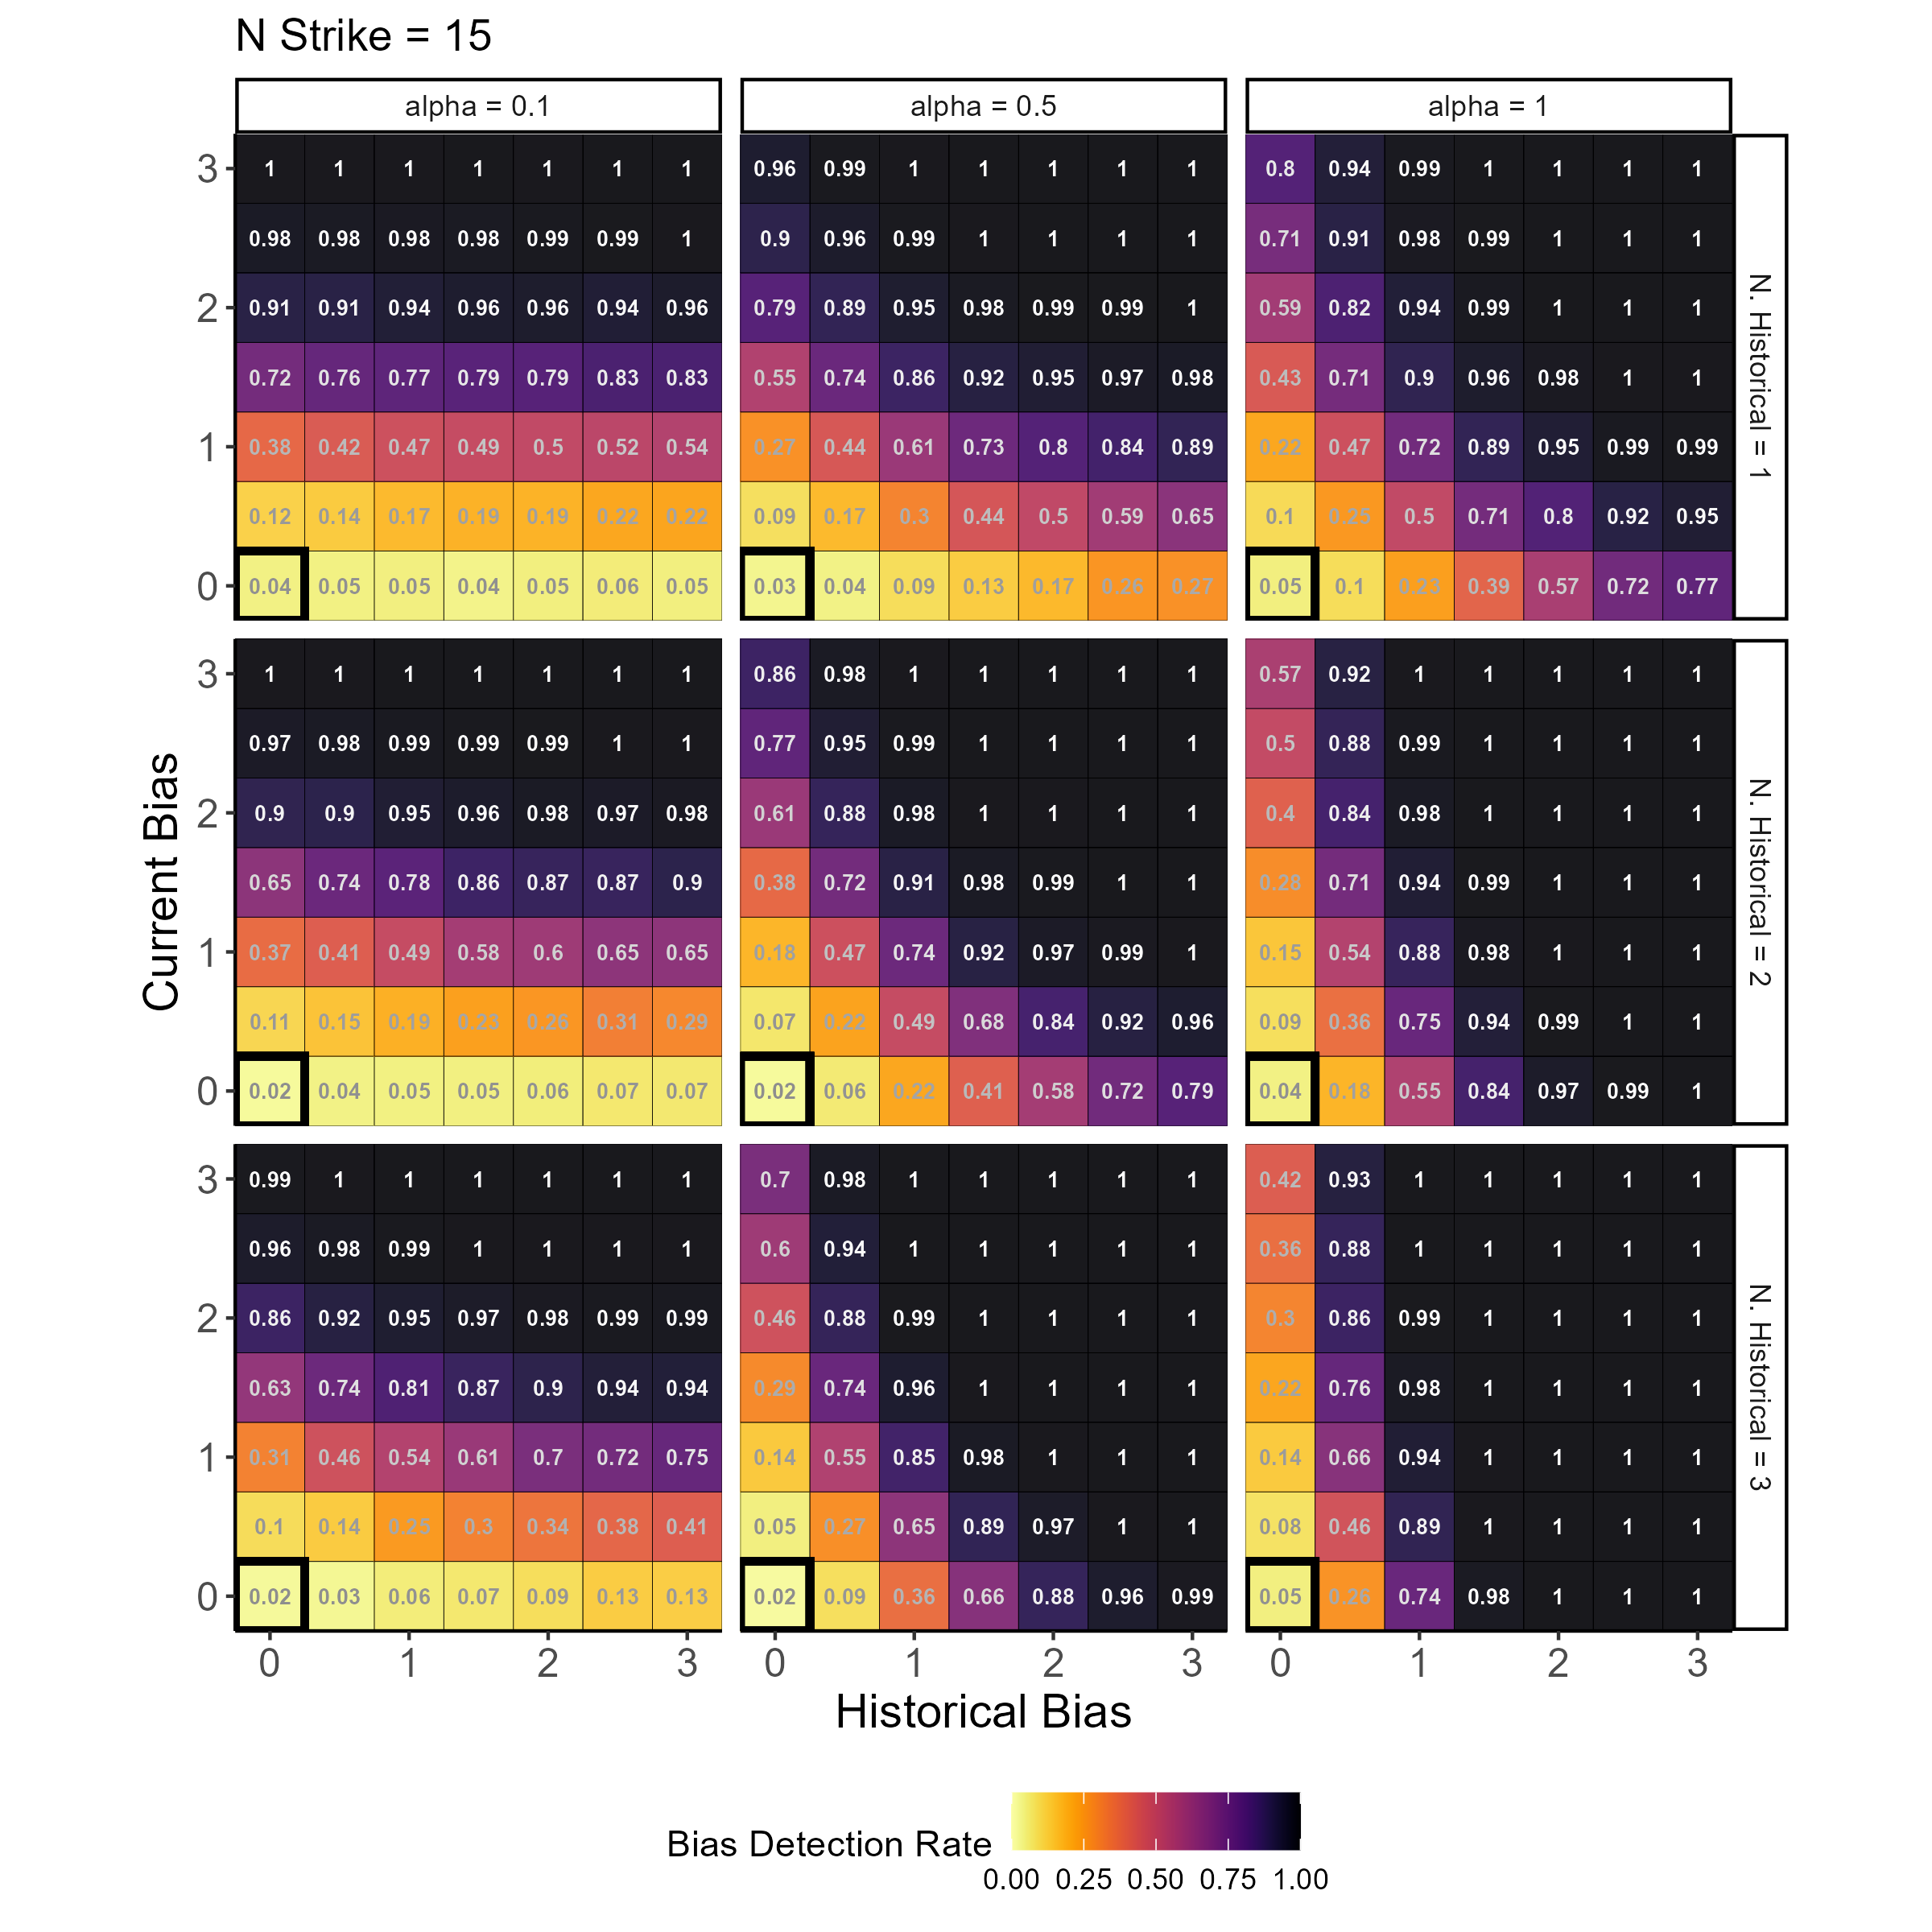
\includegraphics[width=0.95\linewidth]{../figures/pp15_95CI} 

}

\caption{Bias detection rates (proportion of simulations where 0 is excluded from the 95 percent credible interval of bias parameter) for simulations based on 15 strikes. Rows of larger squares correspond to combinations of alpha values (0.1, 0.5, and 1) for low, median and equal weight of historical data to current trial data. Columns of larger squares correspond to 1, 2, or 3 historical trials. Small squares correspond to combinations of bias in current (rows) and historical (columns) trials.}\label{fig:figbd9515}
\end{figure}

\begin{figure}

{\centering 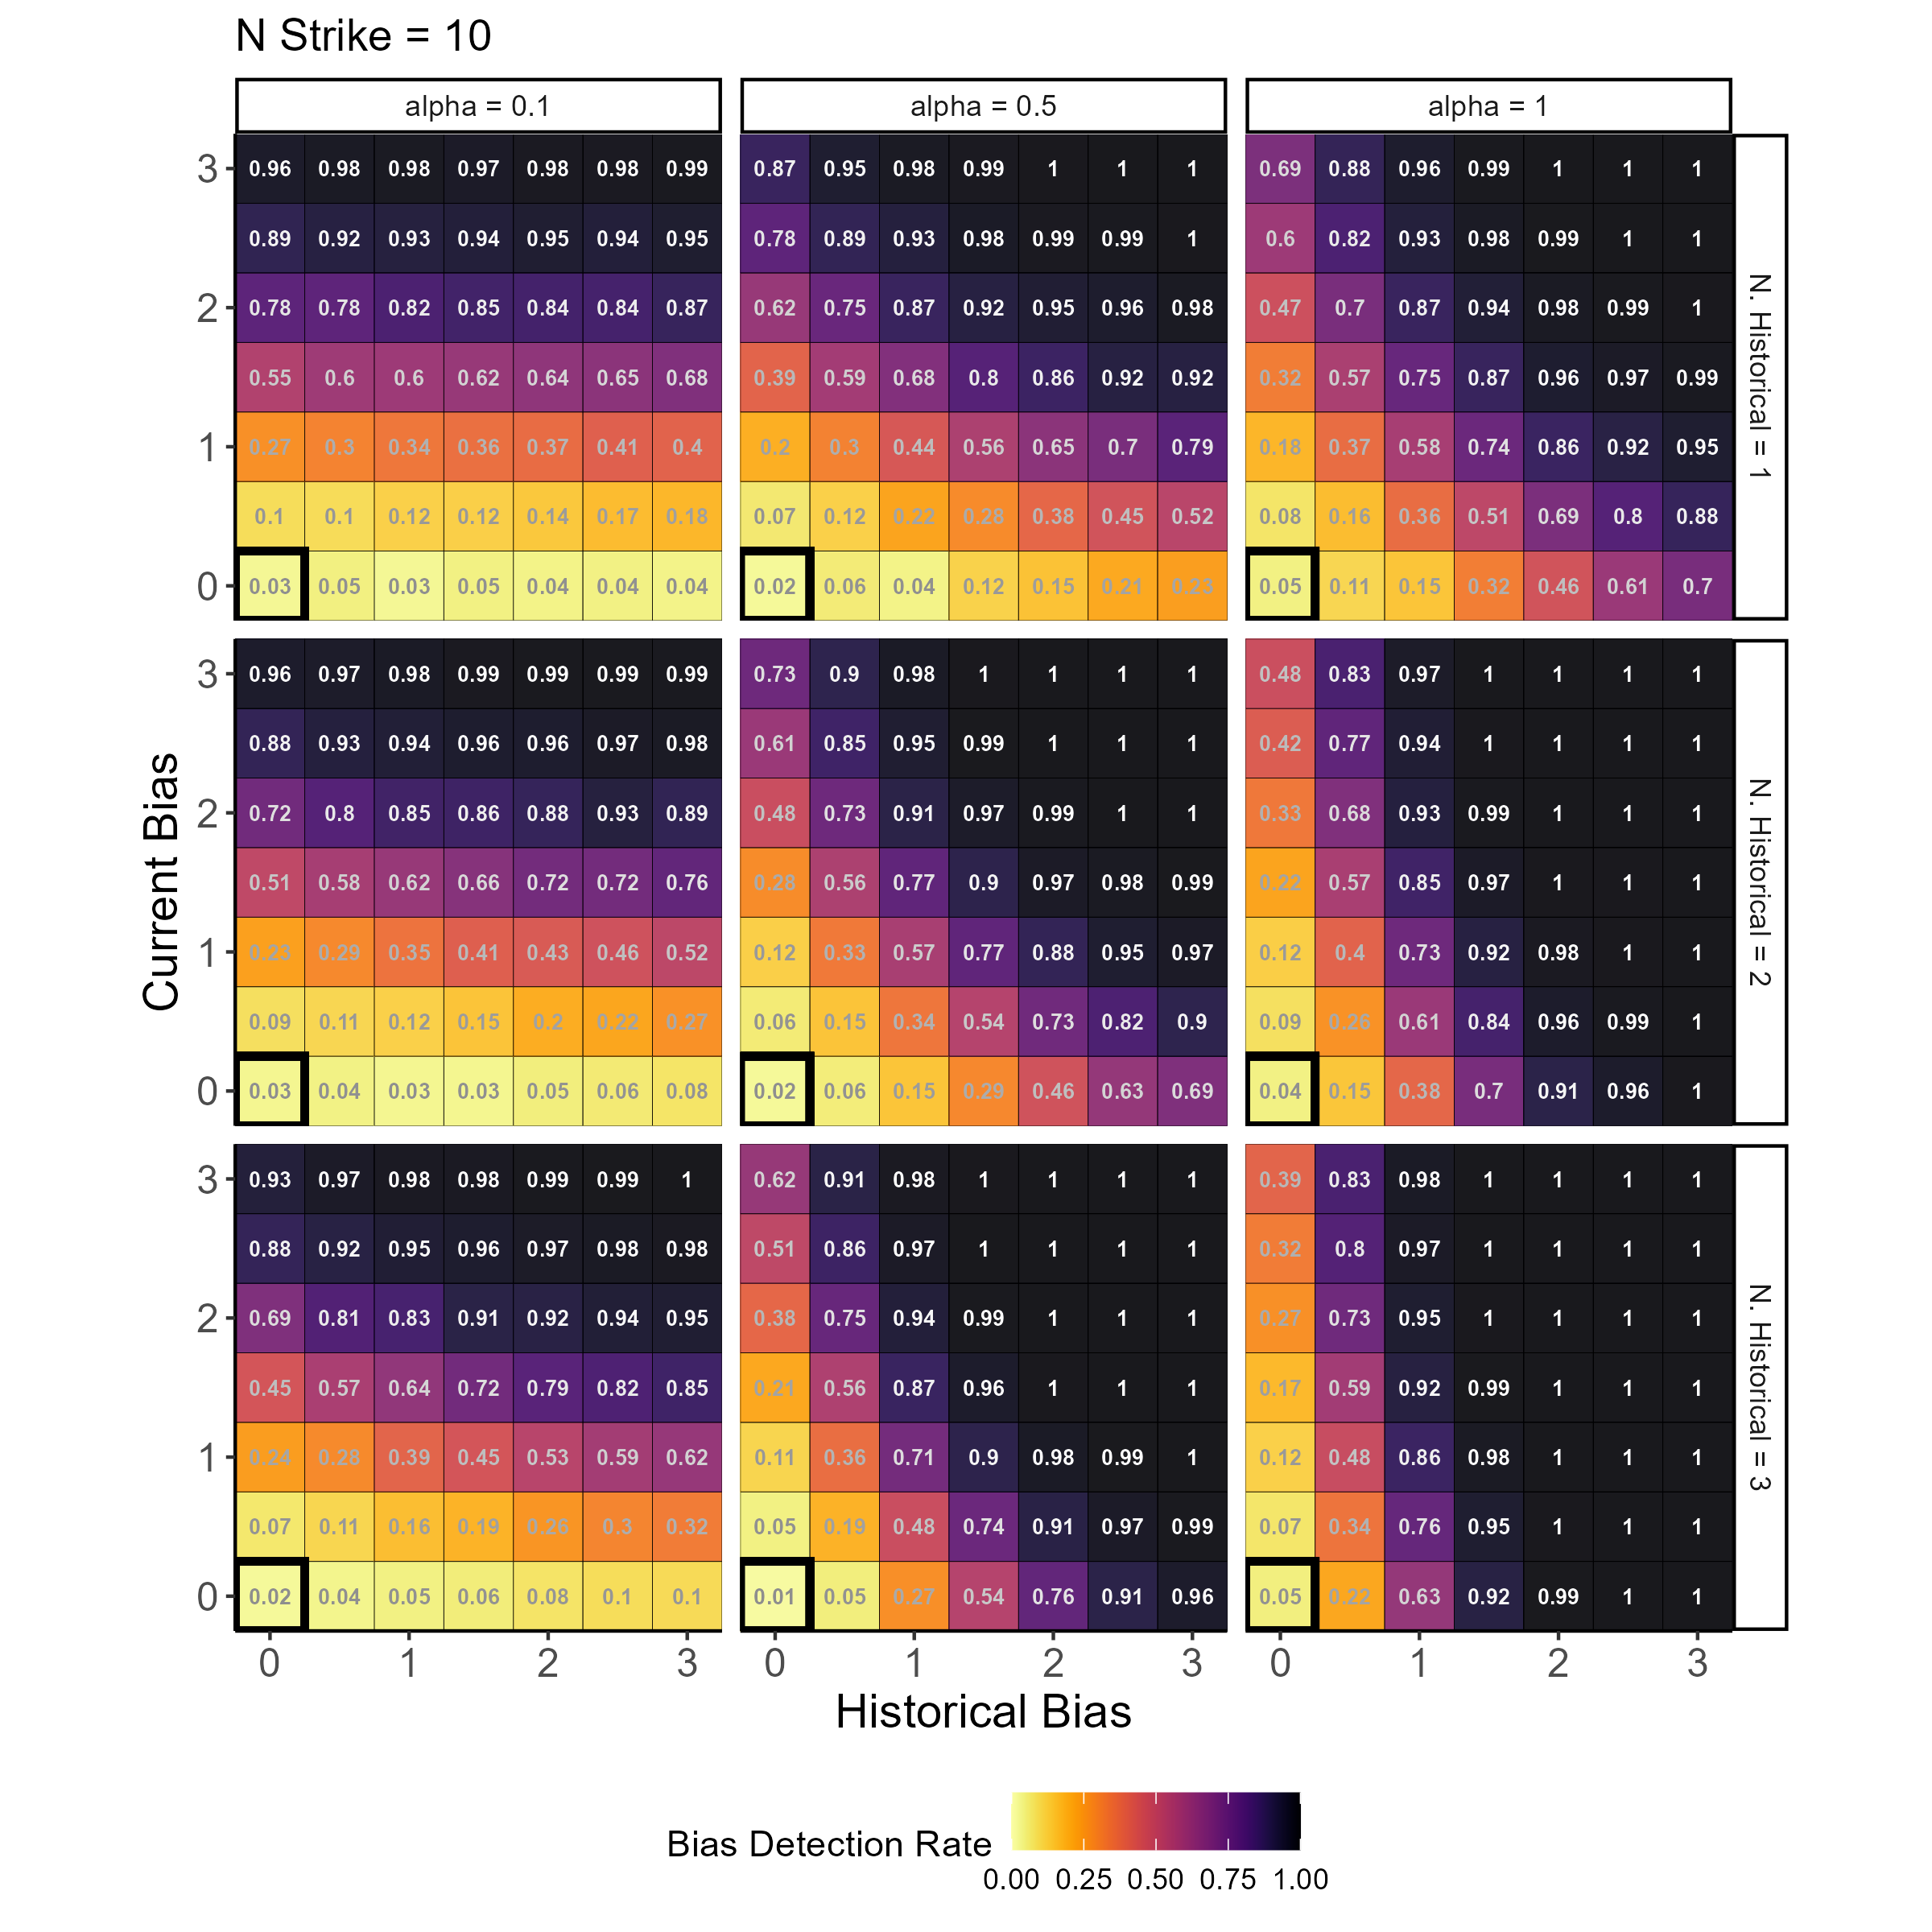
\includegraphics[width=0.95\linewidth]{../figures/pp10_95CI} 

}

\caption{Bias detection rates (proportion of simulations where 0 is excluded from the 95 percent credible interval of bias parameter) for simulations based on 10 strikes.}\label{fig:figbd9510}
\end{figure}

\begin{figure}

{\centering 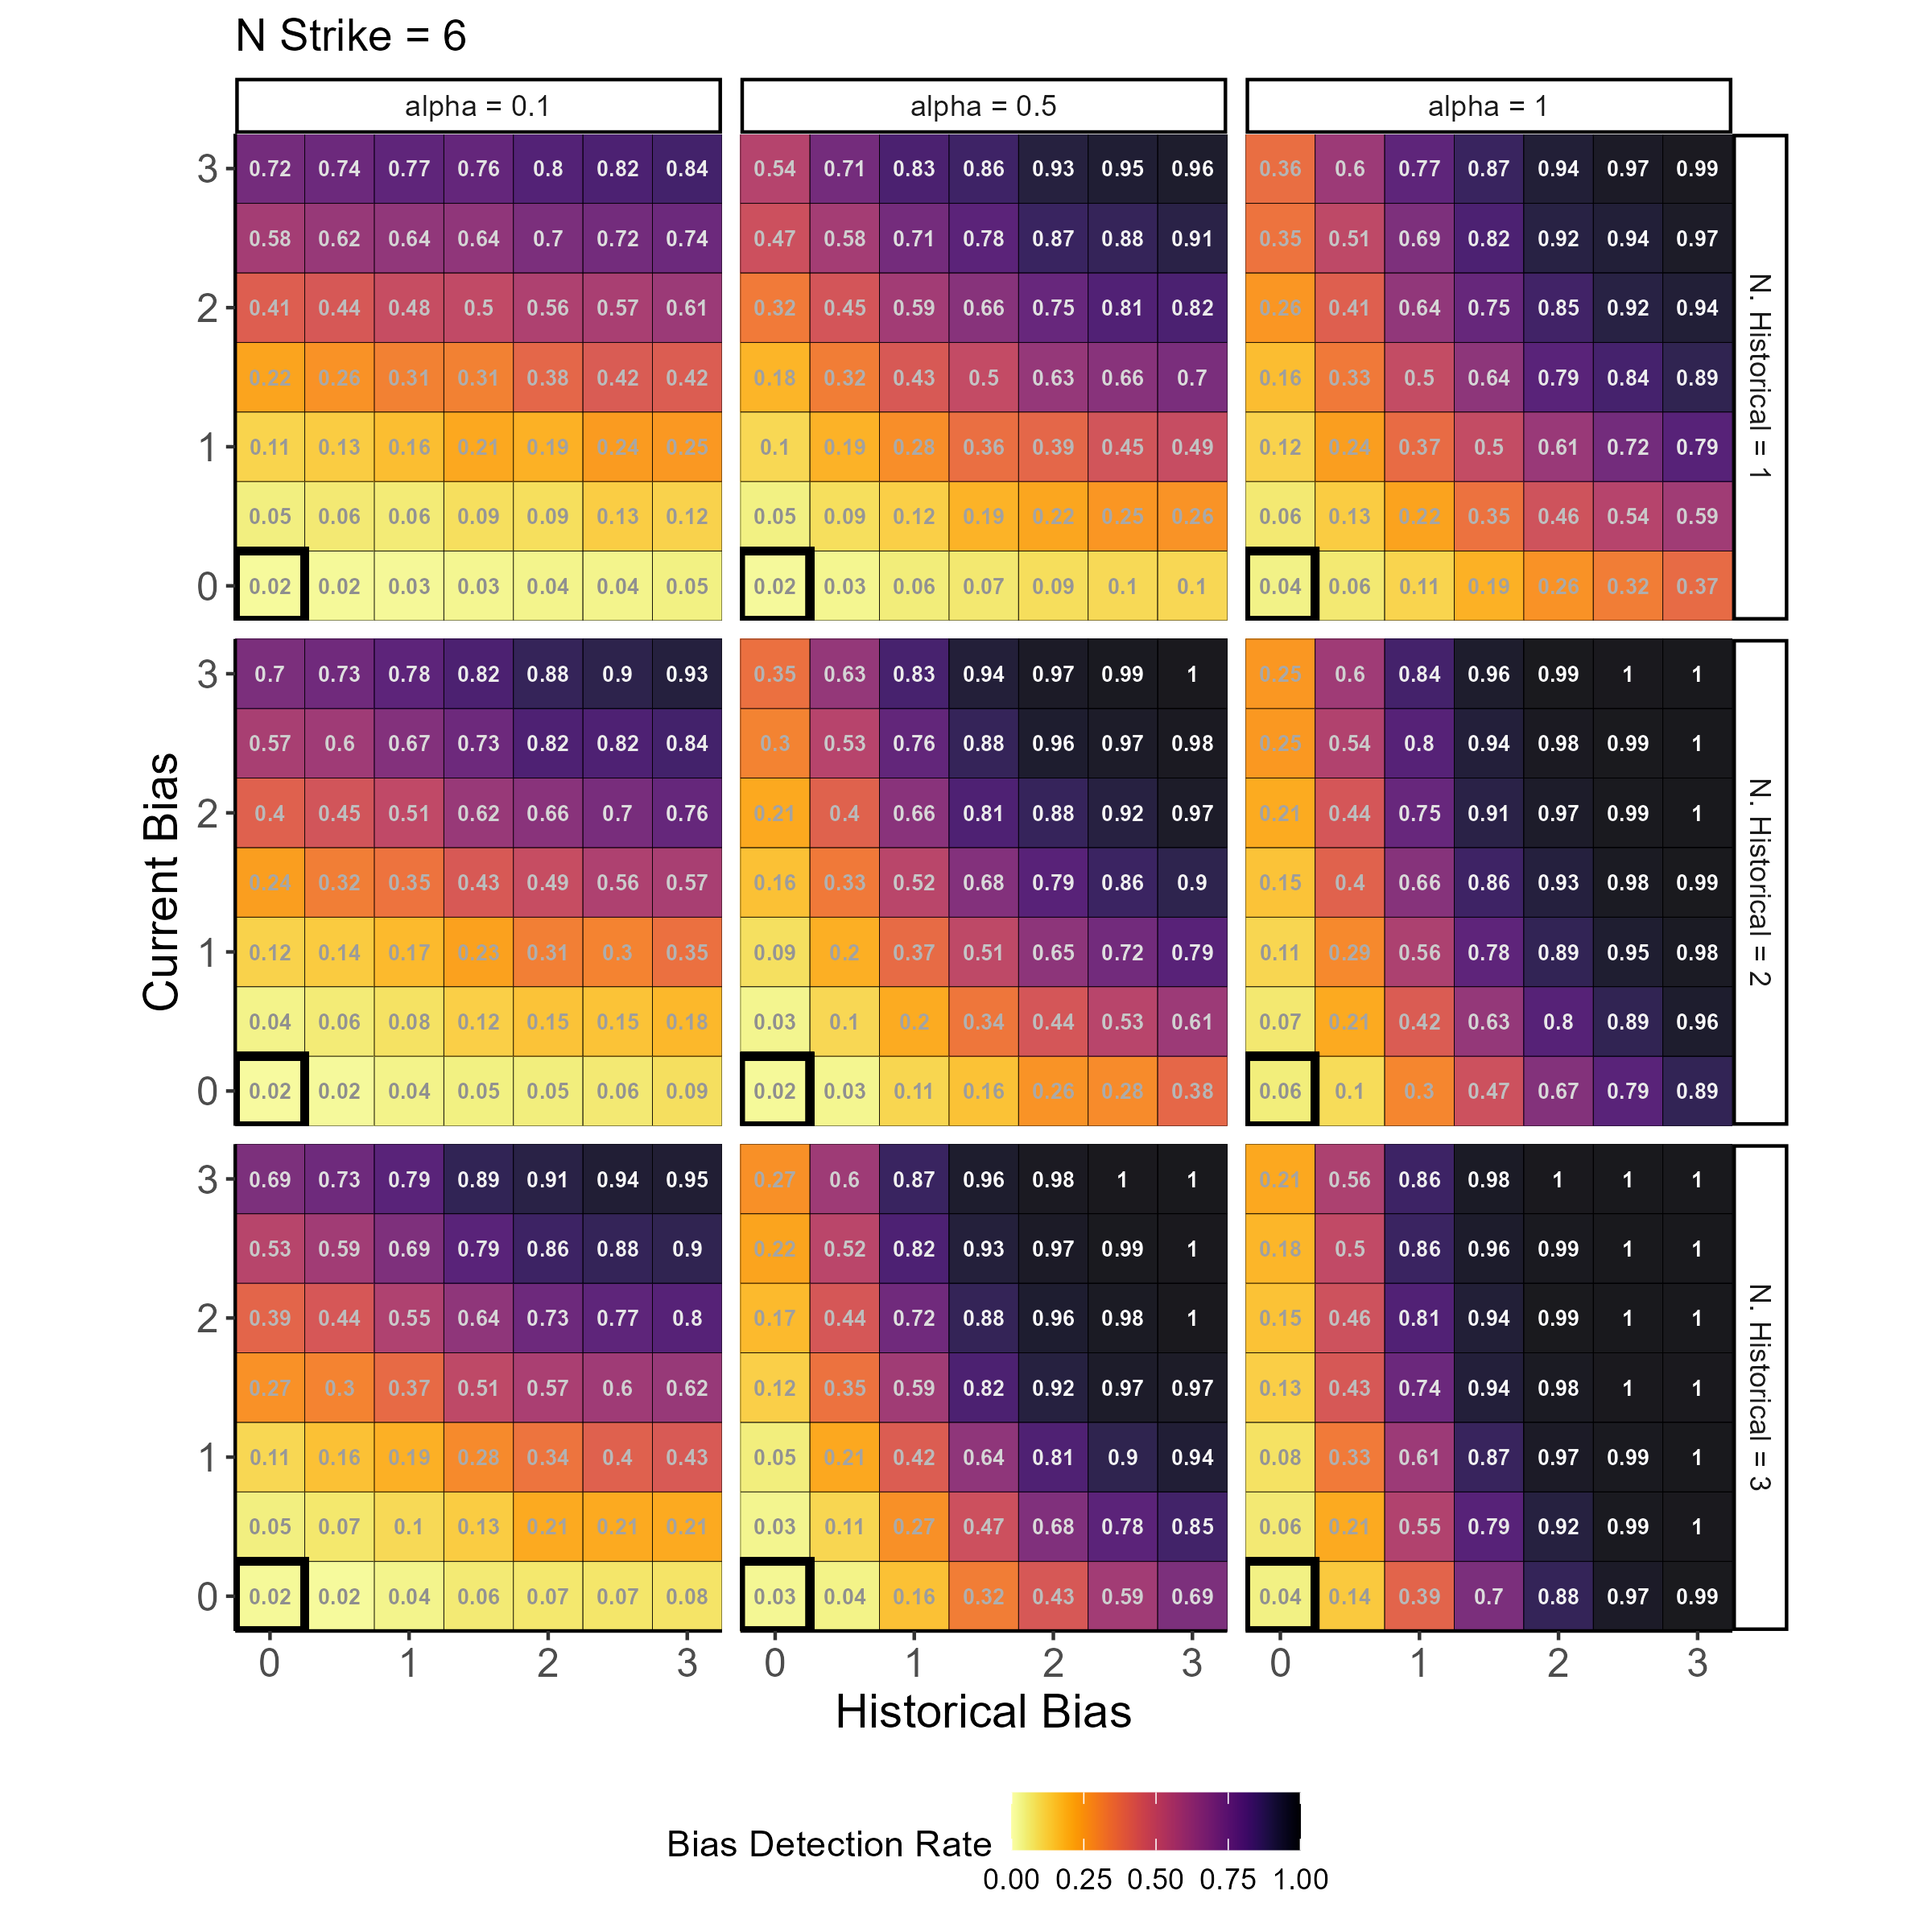
\includegraphics[width=0.95\linewidth]{../figures/pp6_95CI} 

}

\caption{Bias detection rates (proportion of simulations where 0 is excluded from the 95 percent credible interval of bias parameter) for simulations based on 6 strikes.}\label{fig:figbd956}
\end{figure}

As we decrease the number of strikes each attorney has from fifteen to ten and six (Figures \ref{fig:figbd9510} and \ref{fig:figbd956} respectively), bias detection decreases. Bias detection is only high when \(\alpha\) is high (close to 1); current trial bias is high; there is high compatibility between current and historical trials; and the number of historical trials is large.

The choice of credible interval also affects bias detection. For example, with a 90\% credible interval, when \(b_{curr}=2\), the bias-detection rate is lower than with an 80\% credible interval; when \(b_{curr}=0\), that detection rate is higher. The tradeoff is lower accuracy. With a 90\% credible interval, when the bias parameter is 2, the model is less accurate in detecting bias. When the bias parameter is 3, however, the detection rate is still high. For details on simulation results for 90\% and 80\% credible intervals, see the Supplementary Material.

Bias detection will also be sensitive to the choice of the standard deviation of the initial prior (\(\sigma\)). The results above depend in part on our choice of a conservative initial prior for the bias parameter (Equation \eqref{eq:initialprior}). Given little historical strike data for an attorney and a low number of strikes per trial, this initial prior will dominate. As a result, our model will only detect severe bias. This sensitivity, however, reduces after including the historical data, especially when \(\alpha\) is close to 1.

\begin{figure}

{\centering 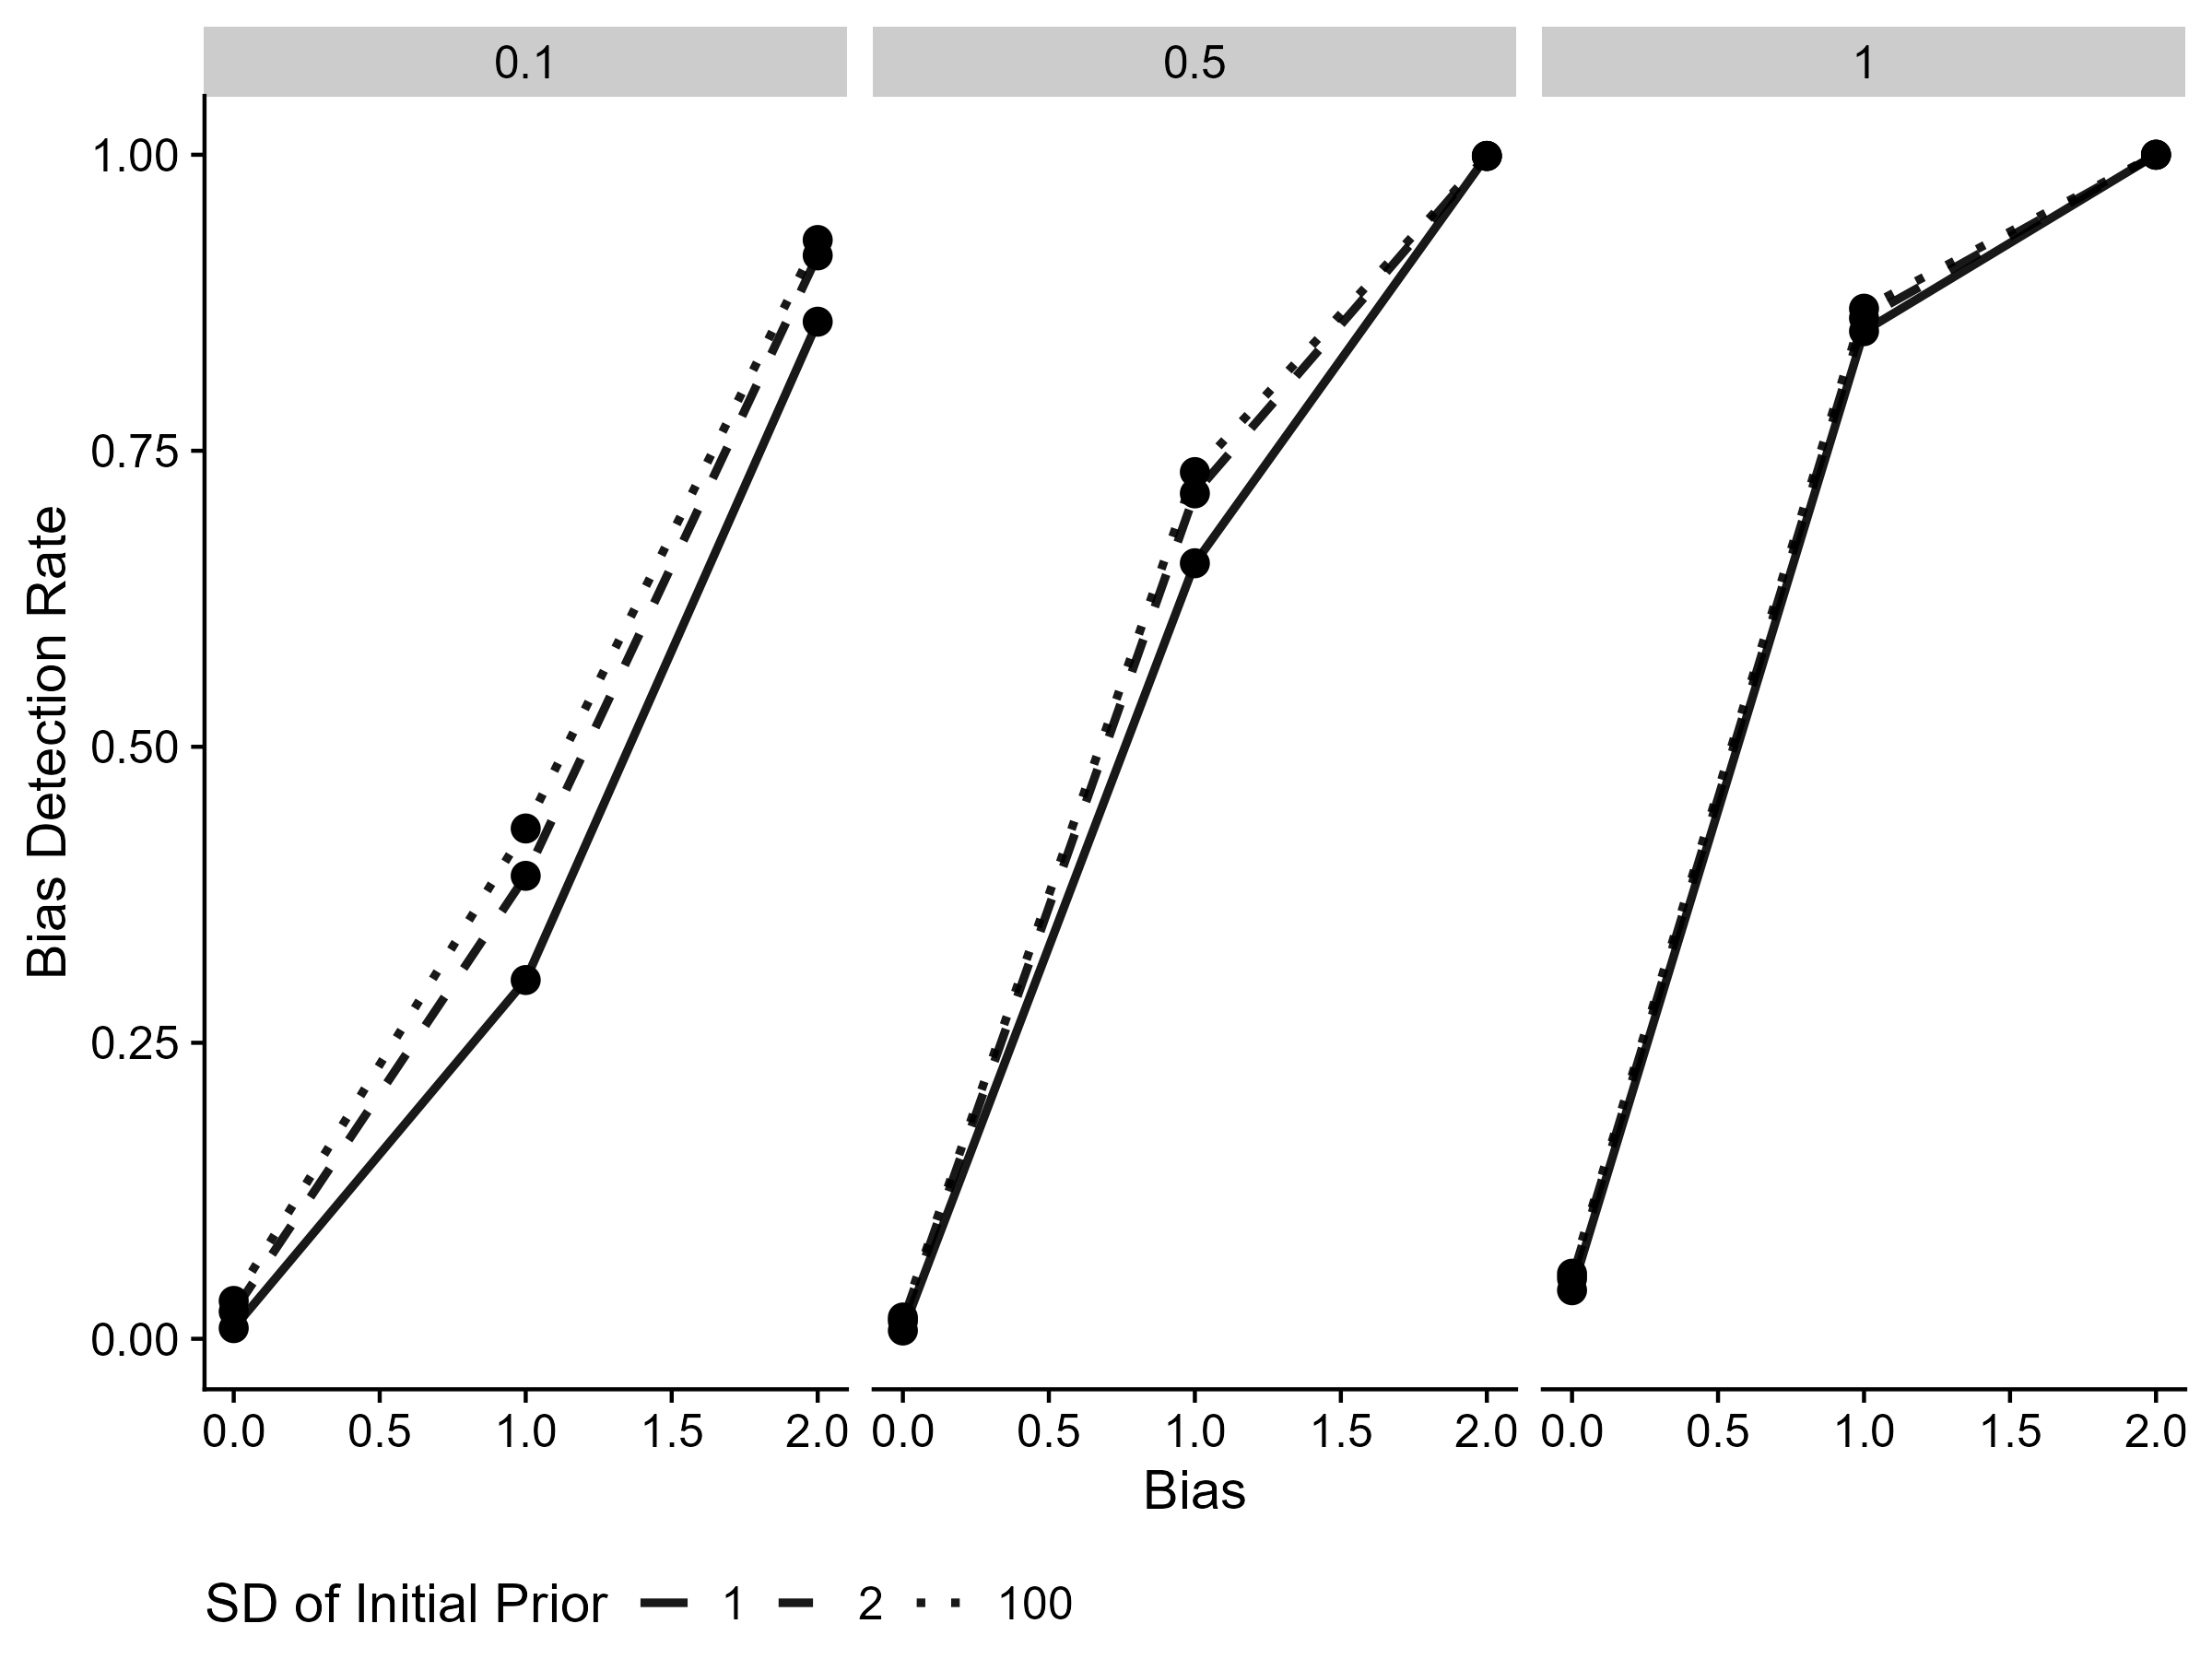
\includegraphics[width=0.8\linewidth]{../figures/SD_sensitivity} 

}

\caption{Sensitivity to Initial Prior's Standard Deviation (SD) by level of discounting (alpha). Simulations were run with 3 levels of the initial prior SD: low (SD = 1), medium (SD = 2), and hight (SD = 100). Bias detection rate corresponds to the proportion of simulations in which bais was detected based on 0 being excluded from the 95 percent credible interval. Bias was equal in current and historical trials and three levels were selected: 0 (no bias scenario), 1, and 2. In general, bias detection is relatively unaffected by choice initial SD, especially when alpha is close to 1.}\label{fig:figsdprior}
\end{figure}

Figure \ref{fig:figsdprior} depicts how assigning different values for the initial prior's standard deviation (\(\sigma = \{1,2,100\}\)) affects the bias detection rate at the 95\% credible interval for three \(\alpha\) values (\(\alpha = \{0.1,0.5,1\}\)) under scenarios where each attorney had 10 strikes and where \(b_{curr} = b_{hist}\). In our simulations, we set \(\sigma = 2\) for our initial prior. If we instead select \(\sigma = 1\), that matters most when \(\alpha = 0.1\), i.e., when we borrow less information from the historical data. As \(\alpha\) increases, the initial prior's standard deviation matters less. Moreover, when we increased the initial prior's standard deviation to make it much less informative (\(\sigma = 100\)), that had little impact on bias detection rates, regardless of the choice of \(\alpha\).

\begin{figure}

{\centering 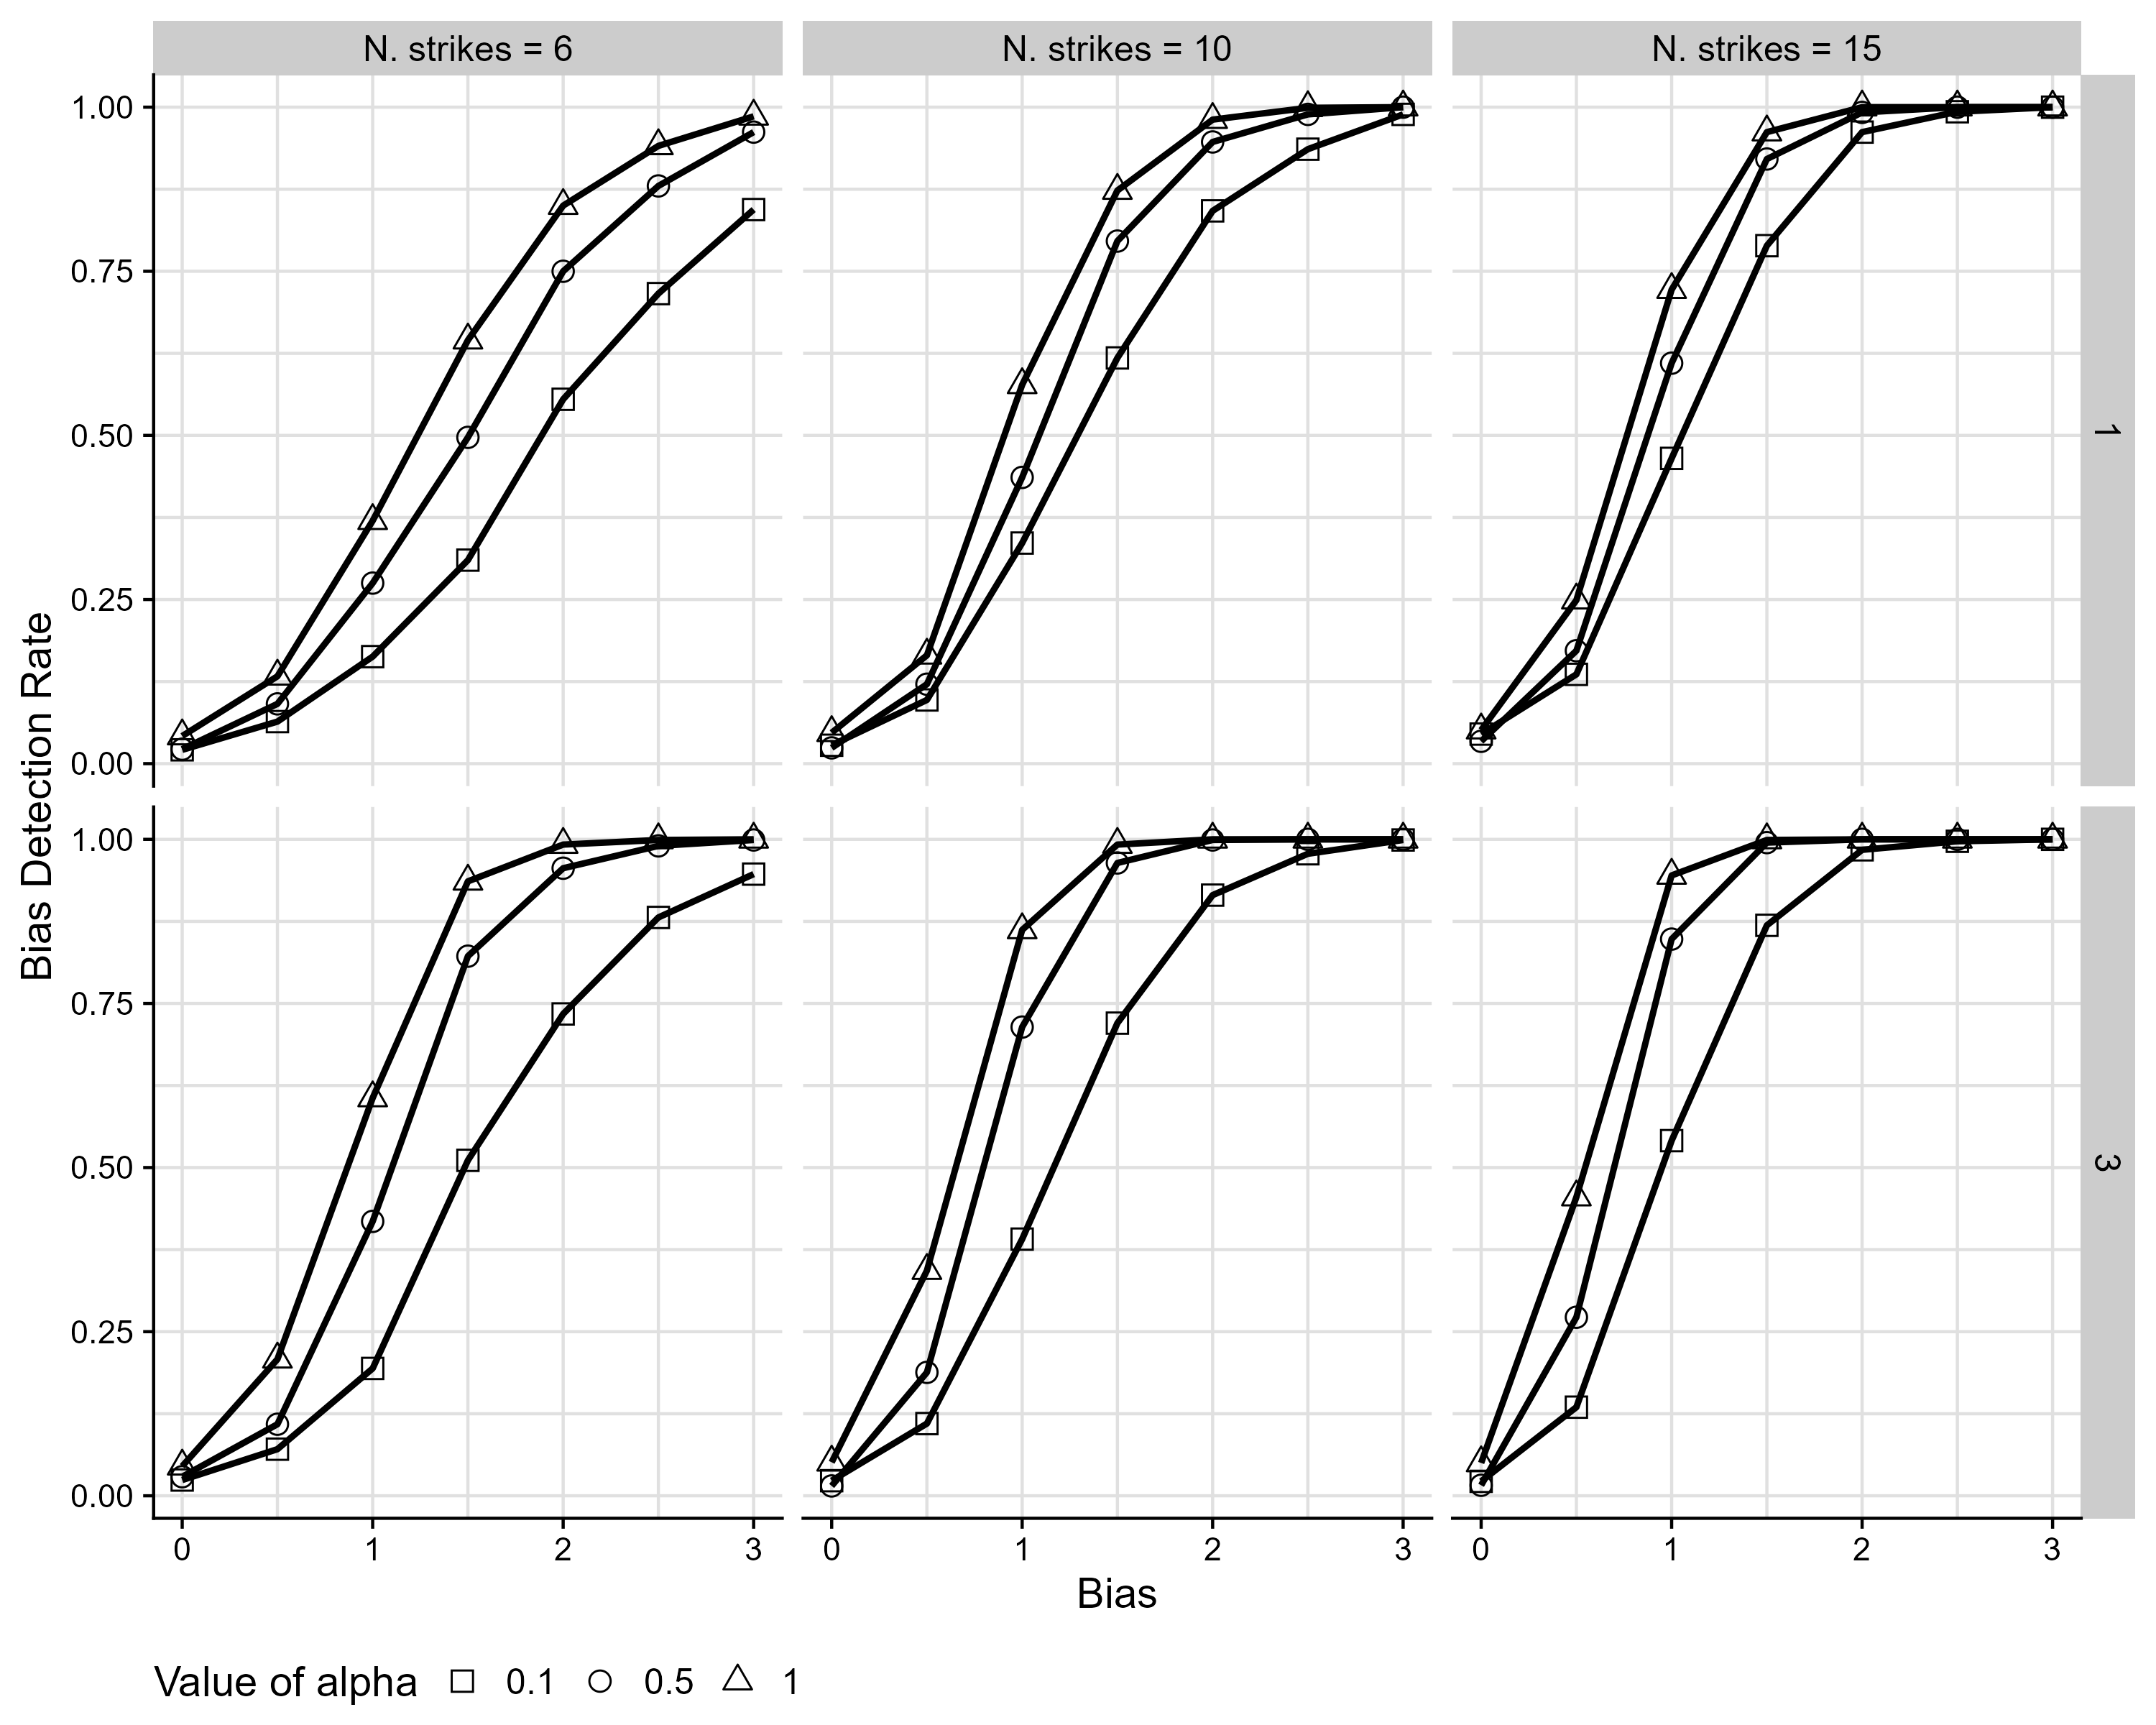
\includegraphics[width=0.85\linewidth]{../figures/compatibility_plot} 

}

\caption{Bias detection under compatibility scenarios (equal bias in current and historical trials) for different numbers of strikes (columns), sizes of historical data (rows) and levels of alpha (shapes). As the weight applied to historical data increases (higher alpha), bias detection increases. Bias detection rates also increase as the number of strikes and historical datasets increase.}\label{fig:figcmptbly}
\end{figure}

Finally, Figure \ref{fig:figcmptbly} summarizes our simulation results for bias detection at the 95\% credible interval, given perfect compatibility (\(b_{curr} = b_{hist}\)). These results indicate that our model can accurately detect strong bias if present in both the current and historical trials. Given high compatibility, increasing \(\alpha\) improves bias detection, as does increasing the number of historical trials and more strikes per trial. Under the low number of strikes per trial (n = 6), bias detection requires strong bias in the current trial and a high \(\alpha\).

\hypertarget{simul-strikes}{%
\subsection{Simultaneous Strikes}\label{simul-strikes}}

In some courts, both parties simultaneously exercise their peremptory challenges on the prospective jurors subject to strikes. This simultaneous-strikes process can be modeled as a special case of the model of an alternating-strikes process above (see Equation \eqref{eq:model3}), i.e, as equivalent to one party engaging in an uninterrupted sequence of strikes against a subset of prospective jurors eligible to be struck. The premise: Regardless of the order in which a party announced those strikes, the posterior for the bias parameter would be the same.

To test this premise, we conducted the following simulation study. We first generated a single trial in which one attorney used fifteen strikes in an uninterrupted sequence against 30 prospective jurors, 15 of which were member of a cognizable-class (e.g., Black jurors). Then, we shuffled the order of those strikes to generate 50 trials with the same proportion of struck cognizable-class members but different orders. We then fit the model to the 50 trials to examine whether the estimated bias parameters across the 50 simulated trials were equivalent.

\begin{figure}

{\centering 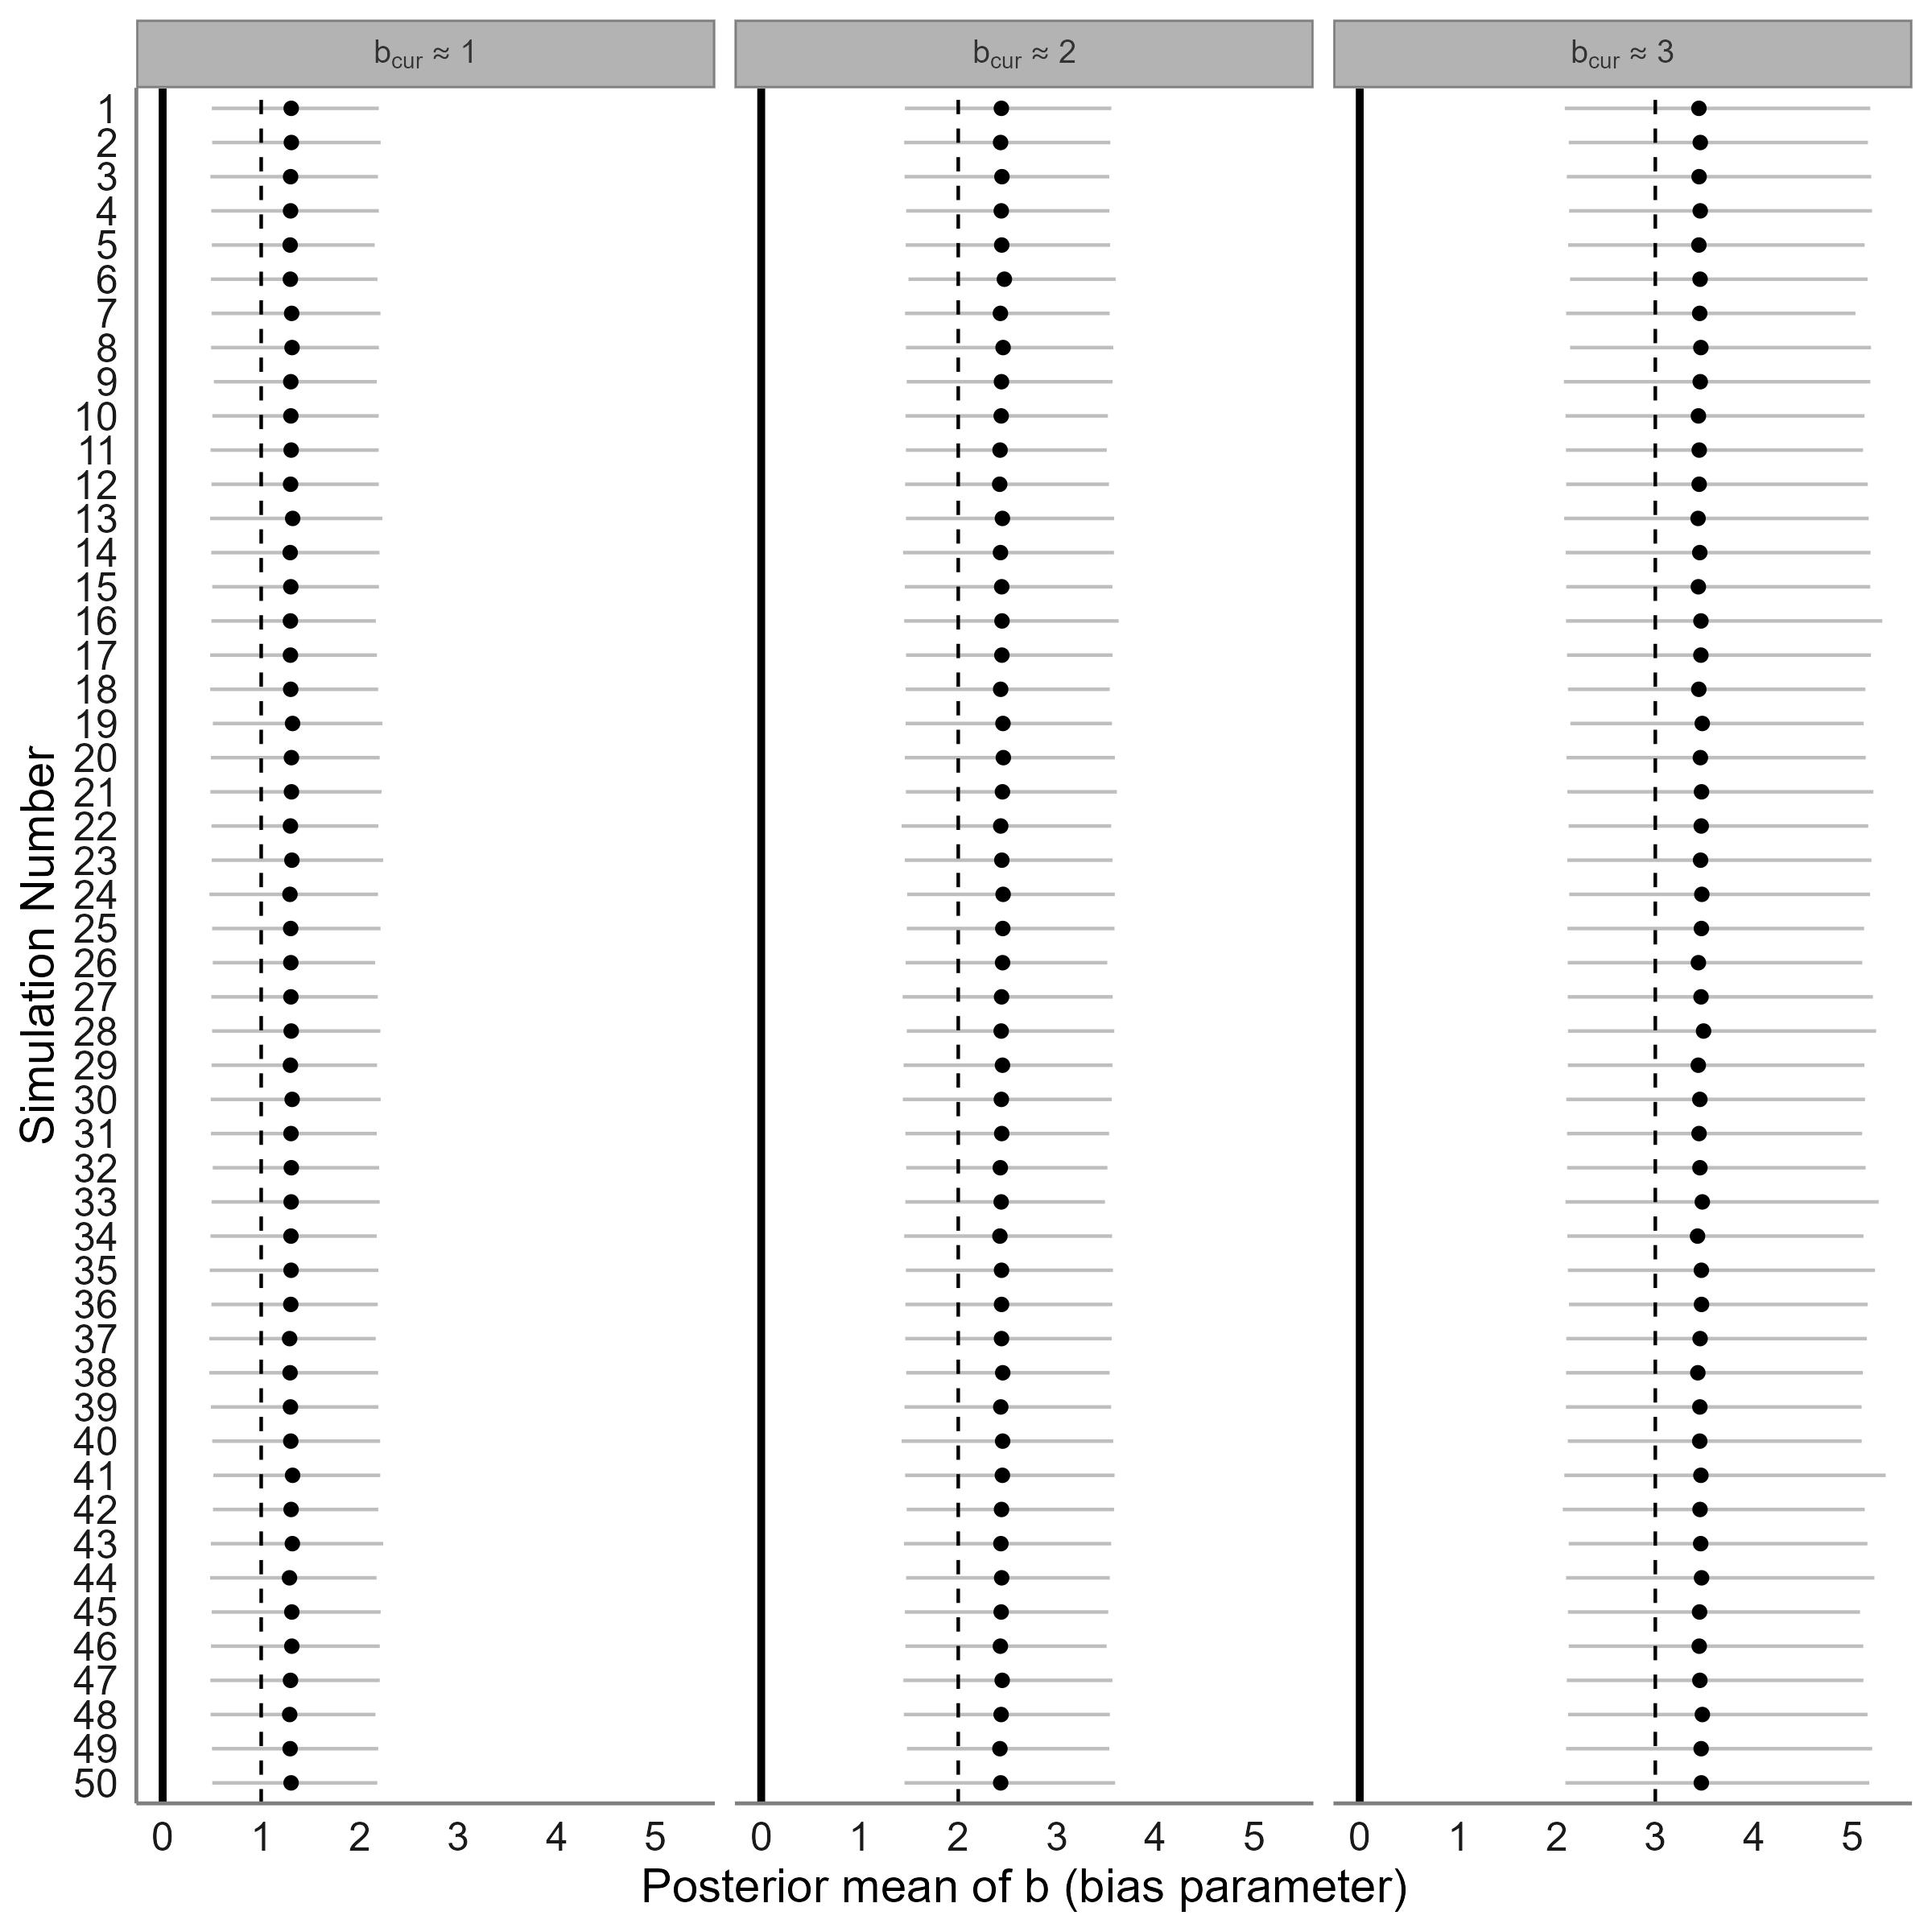
\includegraphics[width=0.75\linewidth]{../figures/simultaneous_sims_plot} 

}

\caption{Simulation results for simultaneous strikes example. Columns correspond to values of bias ($b_{curr}$) used to simulate data. Points and horizontal lines denote estimated posterior mean and 95 pct. credible interval for bias parameter. Vertical dashed lines denote true value of $b_{curr}$ in the simulations.}\label{fig:fig-simul}
\end{figure}

Figure \ref{fig:fig-simul} depicts the results of the simultaneous strike simulations. We find the estimated bias parameter of the 50 trials with different strike orders are close to each other for all of the three scenarios. None of their credible intervals include zero. This shows that the order of strikes does not influence the estimate of the bias parameter. Accordingly, the simultaneous-strikes procedure can be modeled as a special case of our initial model of an alternating-strikes process with an identical likelihood.

\hypertarget{prototype}{%
\subsection{The Software Prototype}\label{prototype}}

We describe here a prototype software application (``app'') that implements the approach described above and that attorneys and others can use in real time to detect bias in the use of peremptory challenges. We built this app with R version 4.3.0 (2023-04-21 ucrt) and the shiny package (R Core Team 2022; Chang et al. 2021). Unlike the simulations, we built the app using Rcpp (Eddelbuettel and Balamuta 2018) and the Metropolis-Hasting algorithm to sample \(b\) from the posterior distribution. As in the simulations, a normal distribution was assumed for the distribution of \(b\). The length of the Markov chain was 110000 and the first 10,000 iterations were dropped as burn-in. No thinning was performed, as the correlation was weak and convergence occurred rapidly. We checked convergence with both traceplots and the Gelman-Rubin statistic (Gelman and Rubin 1992). Computation times vary from 0.76 to 1.2 seconds, depending in the amount of data used (quicker with current strike data only \emph{versus} current plus historical strike data).

To show how lawyers might use this app in real cases in real time during jury selection, we loaded this app with actual strike data from a convenience sample of attorneys who appeared during jury selection in criminal cases in the federal district court for Connecticut during fiscal years 2013 through 2017. Using publicly-available court docket sheets for each case, we matched particular lawyers to these strikes and later assigned them aliases using the charlatan package (Chamberlain and Voytovich 2020). For details on this dataset, see the Supplementary Material.

Next, the user enters by hand the strike information in the case before them in the \emph{strike tally} table (Figure \ref{fig:figapp1}, top left). In the strike tally, \texttt{round} denotes the order of strikes, \texttt{num\_cog} denotes the number of prospective jurors that could be struck that belong to the cognitive class; \texttt{total} denotes the total number of prospective jurors that could be struck; \texttt{cog} indicates whether the prospective juror actually struck in that round was a member of the cognizable class (1 = yes, 0 = no); and \texttt{party} indicates which side used the strike (PP = prosecutor, PD = defense attorney). the user can add or delete rows to the strike tally as needed.

\begin{table}

\caption{\label{tab:inpts}Hypothetical Strike Tally}
\centering
\begin{tabular}[t]{rrrrl}
\toprule
round & num\_cog & total & cog & party\\
\midrule
1 & 5 & 21 & 0 & PP\\
2 & 5 & 20 & 1 & PD\\
3 & 4 & 19 & 1 & PP\\
4 & 3 & 18 & 0 & PD\\
5 & 2 & 17 & 0 & PP\\
\addlinespace
6 & 2 & 16 & 1 & PD\\
7 & 2 & 15 & 1 & PP\\
8 & 2 & 14 & 0 & PD\\
9 & 2 & 13 & 0 & PP\\
10 & 2 & 12 & 0 & PD\\
\bottomrule
\end{tabular}
\end{table}

To illustrate, suppose the strike tally in Table 1 depicts the pattern of strikes in the present case with defense attorney Aaron Waelchi and prosecutor Lawrance Klocko V (both aliases for actual attorneys in the historical strike data). After the user enters this strike tally, the app initially displays two graphs -- one for the prosecution and the defense. Each graph depicts the prior density plot (colored light grey) and posterior density plot (blue and red for defense and prosecution, respectively) for the bias parameter (Figure \ref{fig:figapp1}(a)). Here, the 95\% credible interval includes zero, indicating no credible basis to infer bias, given the current strike tally alone. In the default setting, the pull-down menus for prosecutor and defense are set to ``None''. As a result, the app ignores any historical strike data and estimates the posterior distributions of the bias parameter for this prosecutor and defense attorney based only on the strike tally data and the initial prior (\(b \sim N(0,2)\)).

\begin{figure}

{\centering \subfloat[Current Strike Data only\label{fig:figapp1-1}]{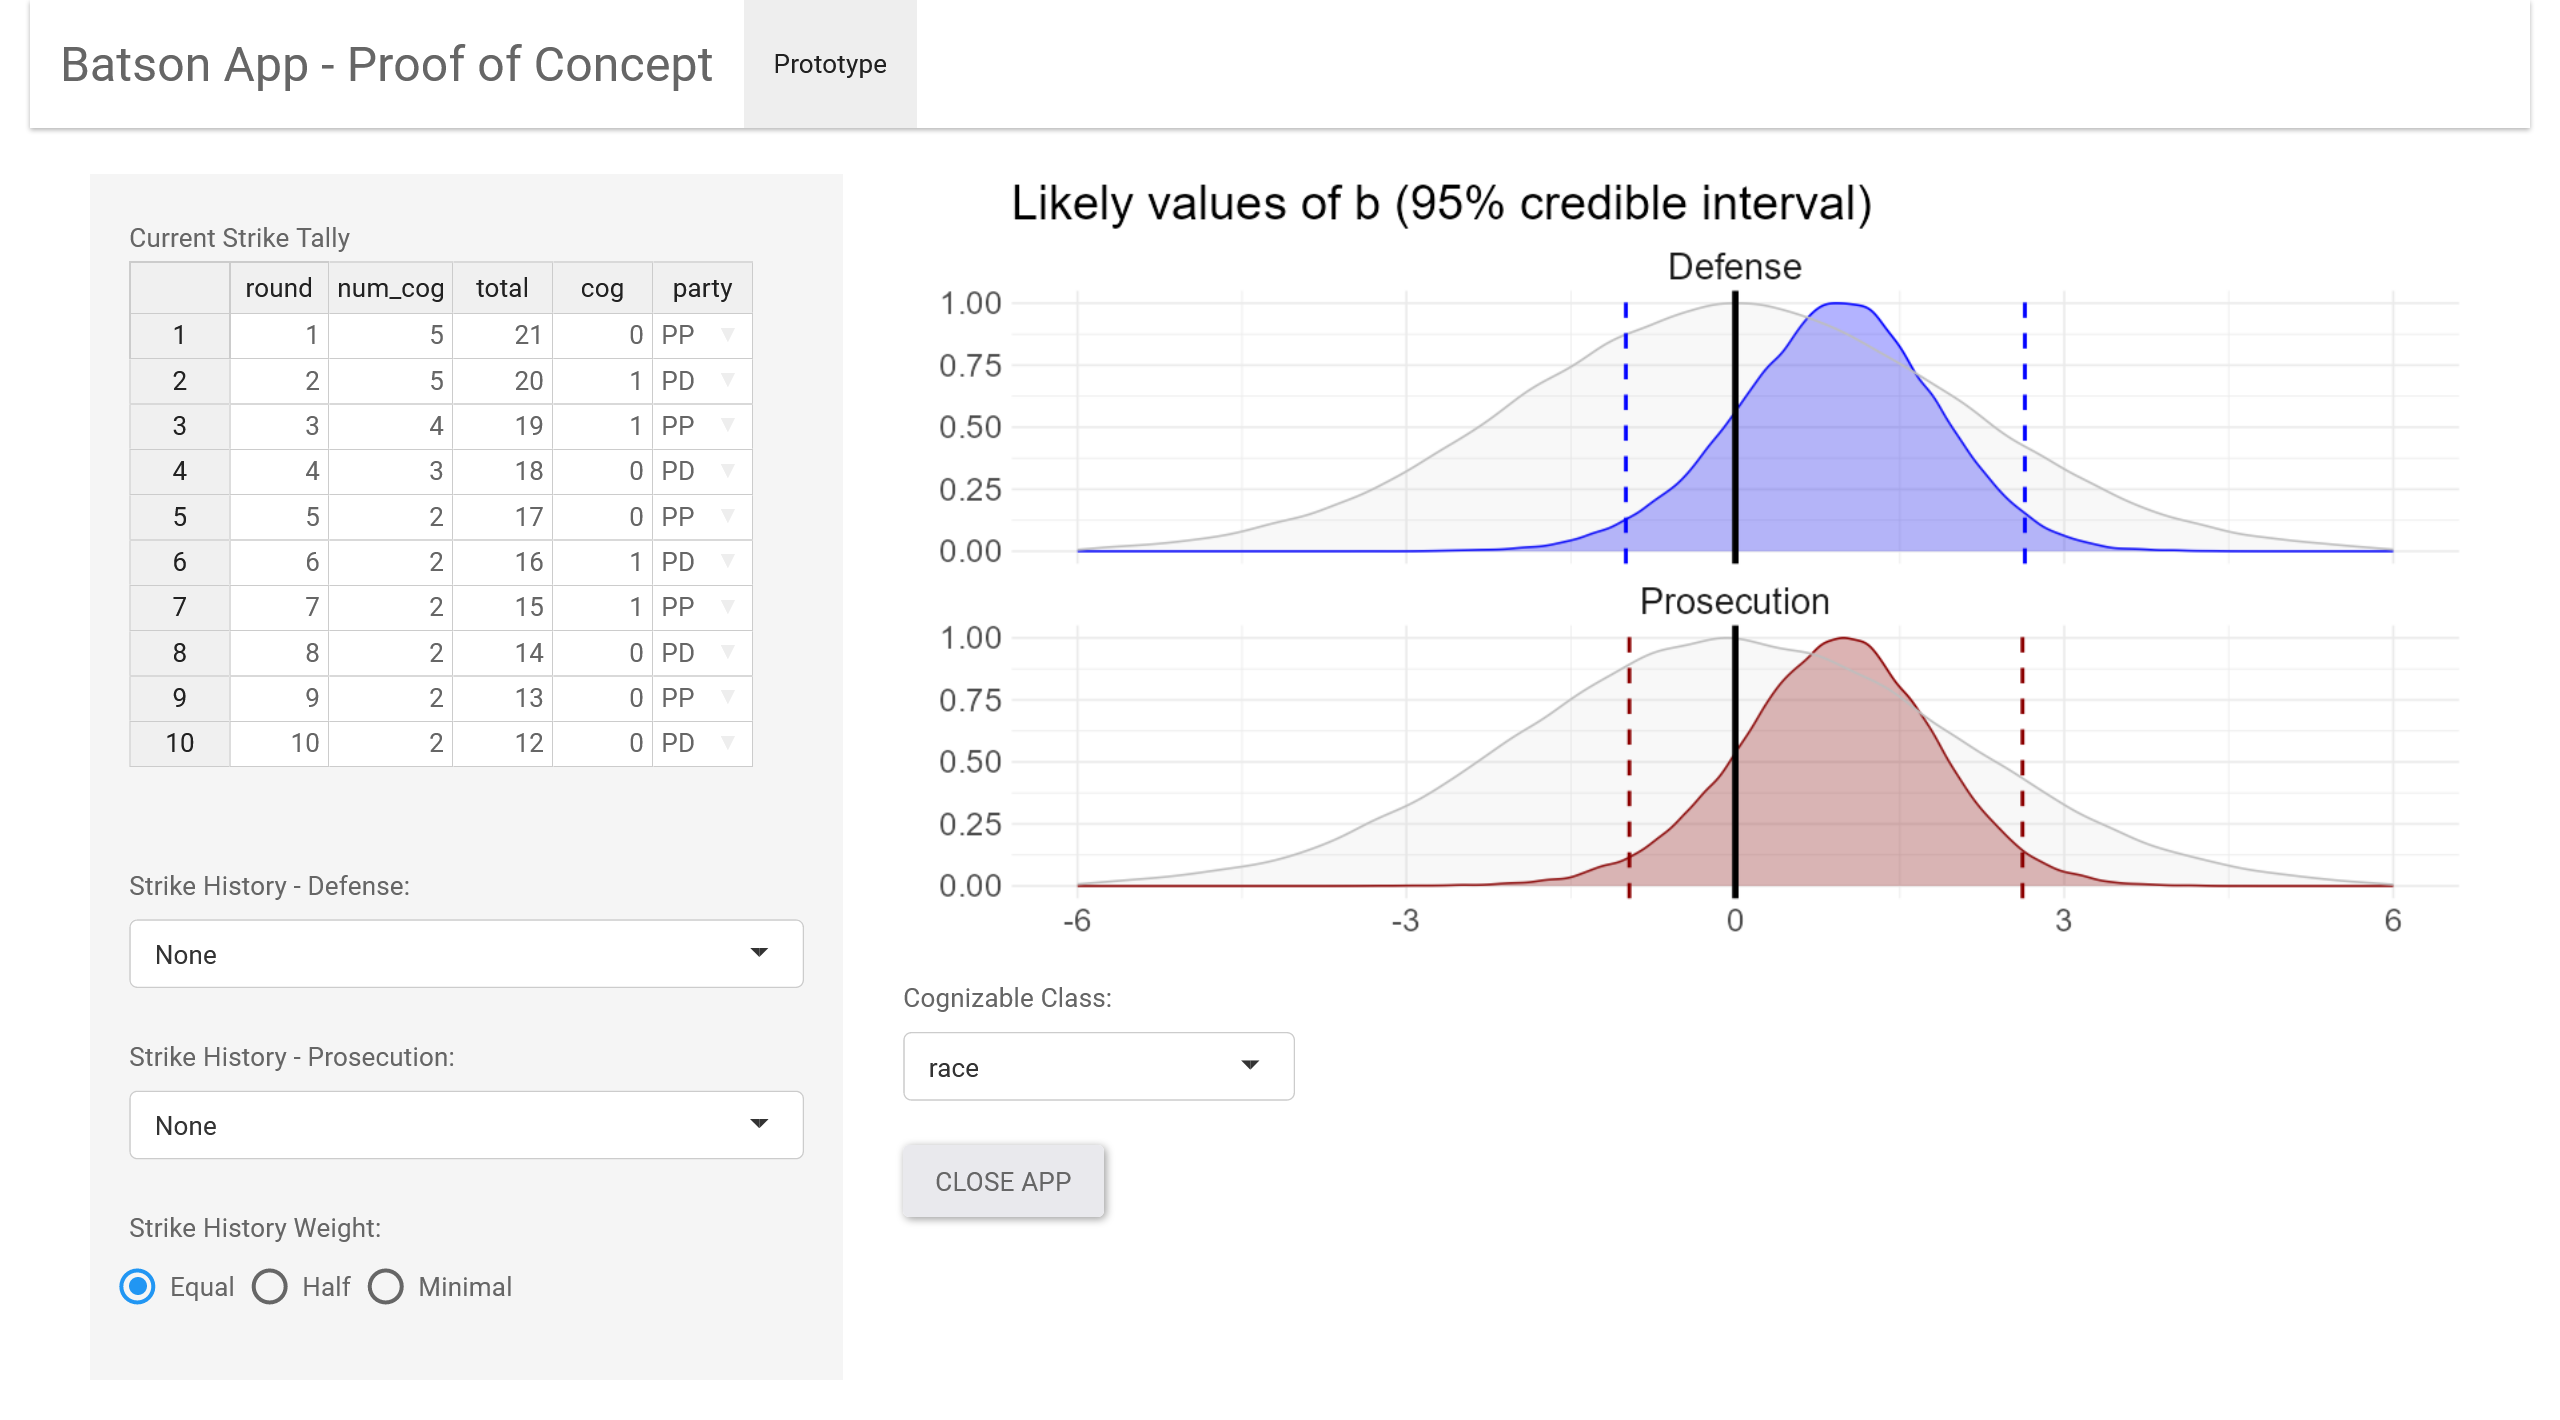
\includegraphics[width=0.5\linewidth]{../figures/batson_app_screenshots/batson_app_screenshot1} }\subfloat[Historical and current strike data\label{fig:figapp1-2}]{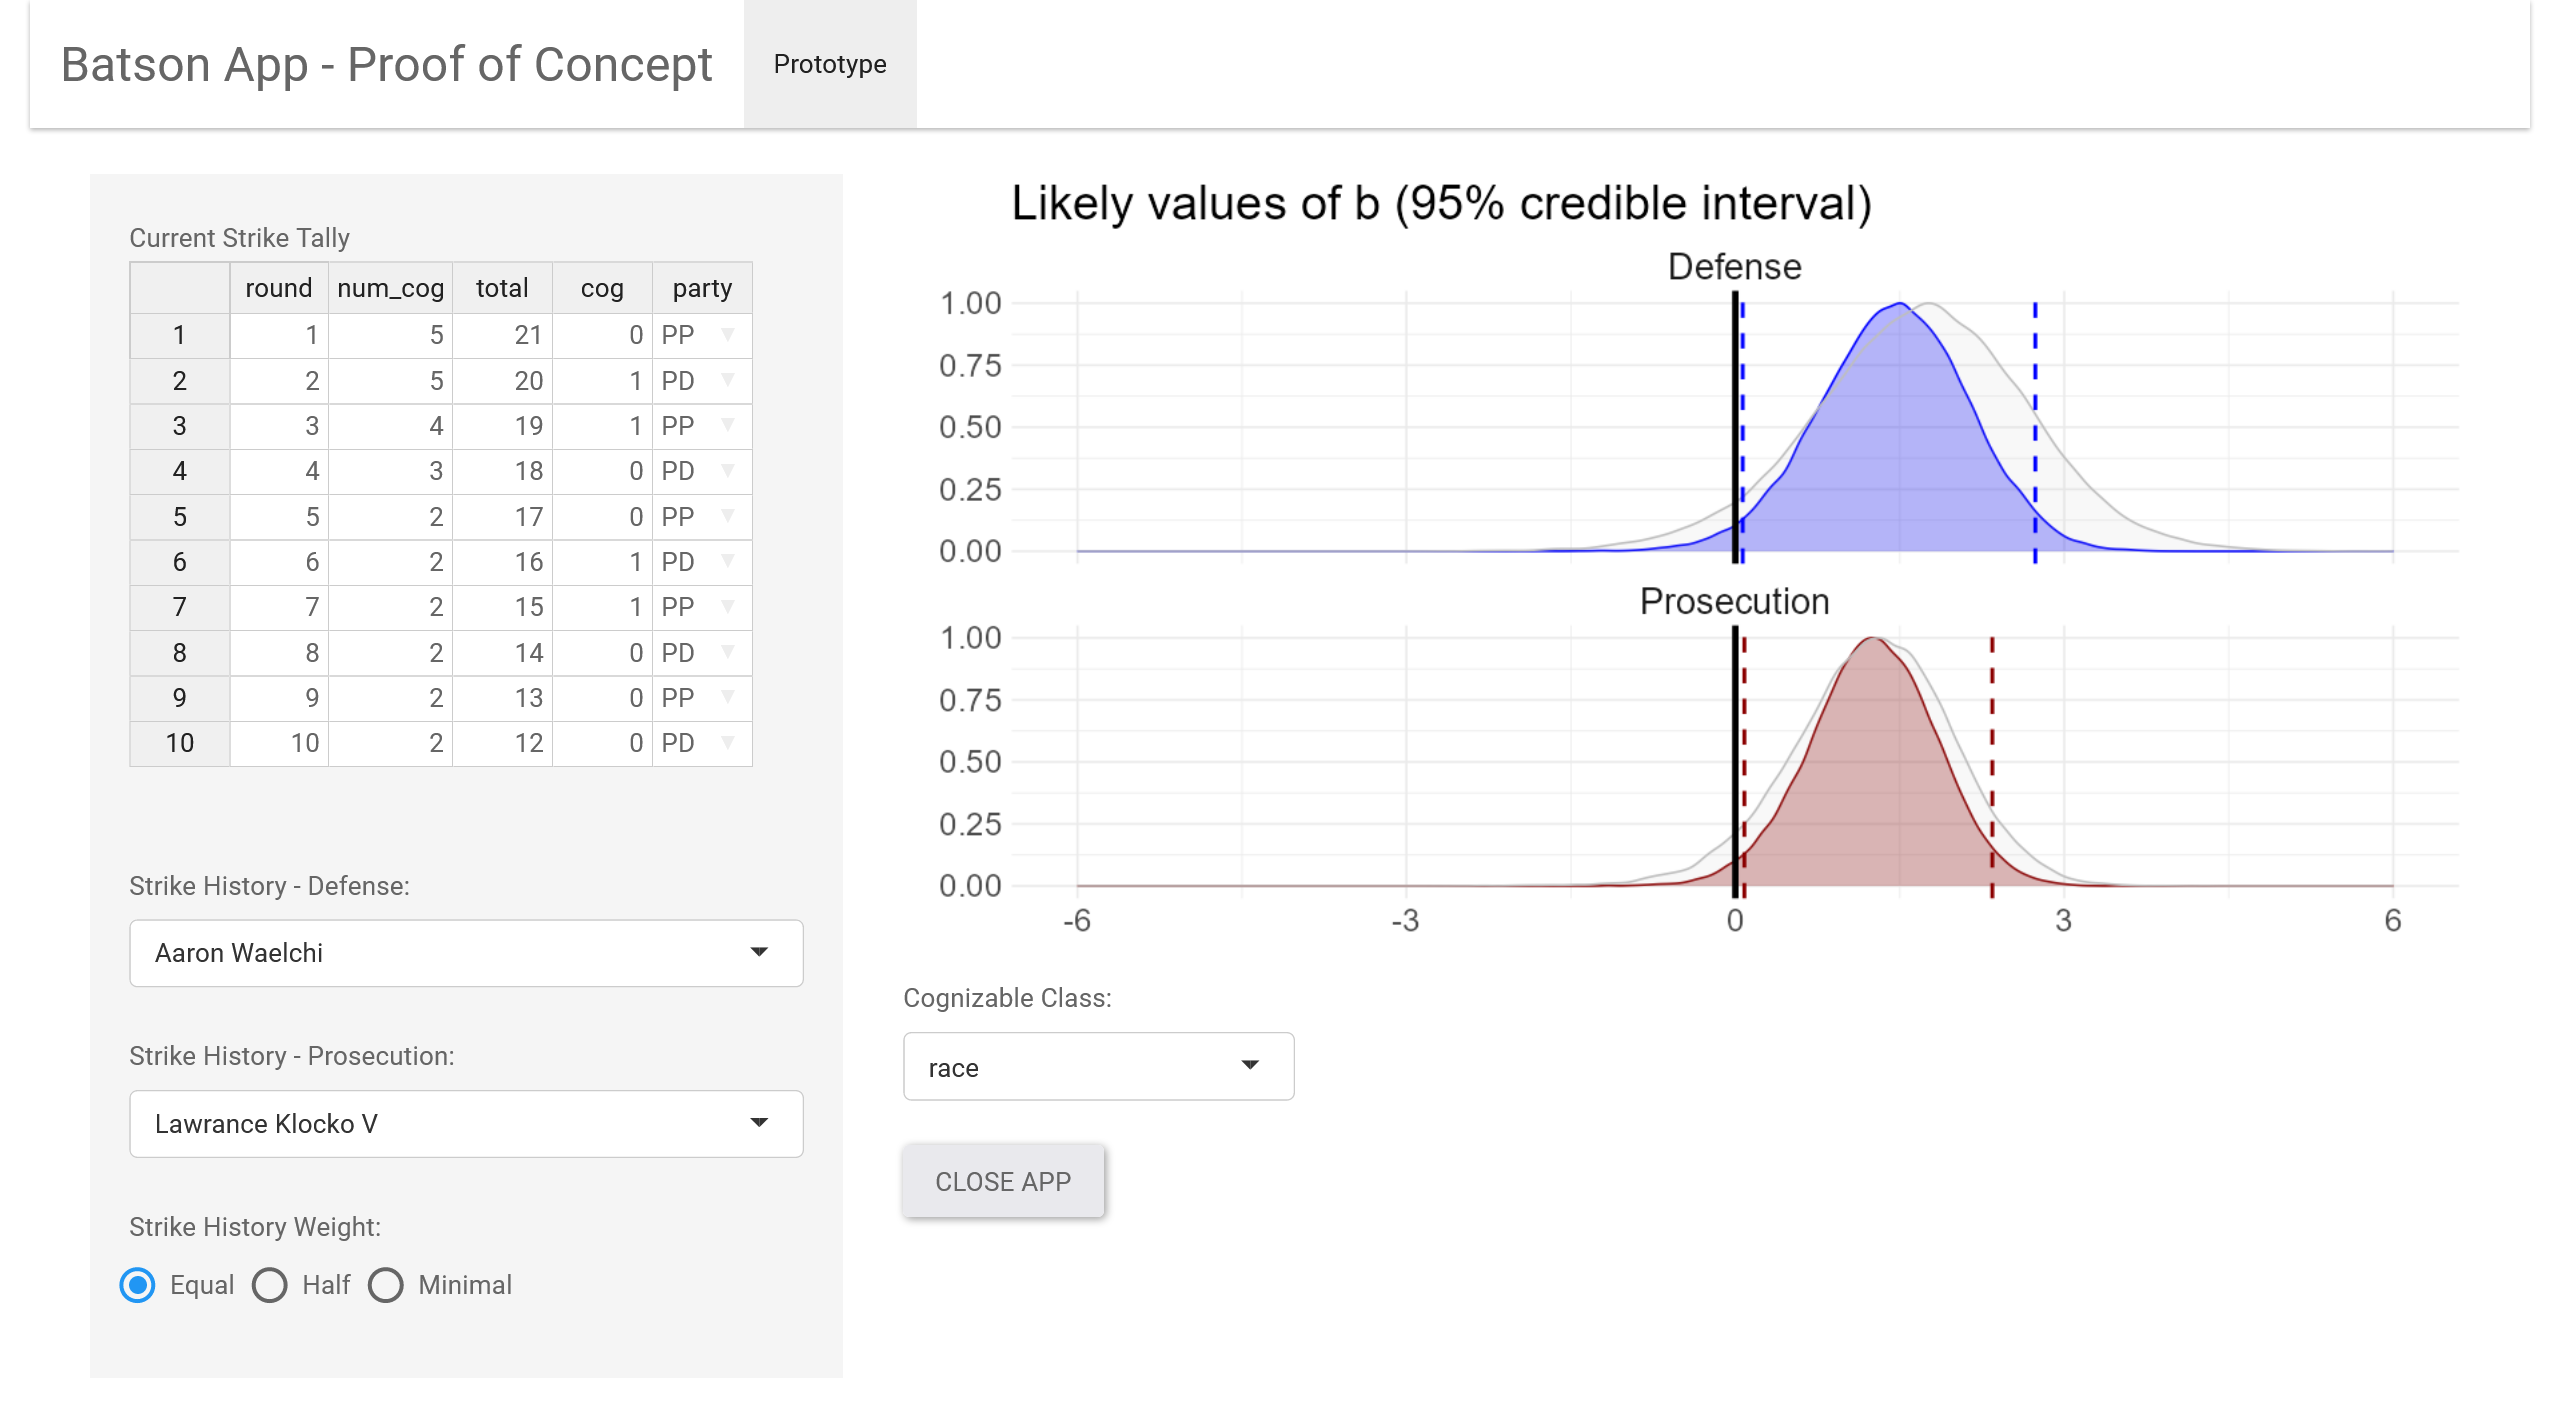
\includegraphics[width=0.5\linewidth]{../figures/batson_app_screenshots/batson_app_screenshot2} }

}

\caption{Screenshots of R-Shiny application showing density plots for race bias of prosecutor and defense attorney. Vertical dotted lines depict 95 pct. credible interval. Blue and red density plots represent draws from posterior distributions of defense attorneys and prosecutors respectively. Grey background density plots show the initial priors (before using current strike pattern). (a) shows the result when no historical data are included, and (b) shows the result when historical data are included with equal weight to current data ('Strike History Weight' set to 'Equal', i.e., alpha = 1).}\label{fig:figapp1}
\end{figure}

To use historical strike data, the user selects the name of the prosecutor or defense attorney from the pull-down menus. If an attorney's name cannot be found, the app has no historical strike data for that attorney. Once selected, the prior and posterior density plots automatically update to account for the pre-loaded historical strike data for that attorney. For the weight to assign that attorney's historical strike data, the default is set to equal weight of historical information and current information (\(\alpha = 1\)). The user has two other options: half weight (\(\alpha = 0.5\)) and minimal weight (\(\alpha = 0.2\)).

In our illustration, we select the names of the prosecutor and defense attorney from their respective pull-down menus; and leave the weight setting to ``Equal''. The density plots update accordingly (Figure \ref{fig:figapp1}(b)). Now the credible intervals clearly exclude zero. Thus, we have a credible basis to infer bias against racial-minority prospective jurors in how these attorney use their peremptory challenges in the present case. In the Supplementary Material, we present additional illustrations wherein we use the app to detect gender bias and where we assign less weight to the historical strike data.

\hypertarget{discussion}{%
\section{Discussion}\label{discussion}}

Statistical methods for \emph{Batson} and similar challenges often use historical strike data to infer illegal strike bias. The Bayesian approach presented here accounts for available historical strike data when estimating the posterior for the bias parameter. By incorporating the power prior, this approach makes assumptions about the incompatibility between current and historical trial data an explicit part of the process of identifying bias and the decision of whether to bring a \emph{Batson} challenge or not. Moreover, with a tool like our prototype app, attorneys can use the approach presented here in real time during jury selection to help them decide whether to make a \emph{Batson} challenge at all. If argued, the attorney can also introduce that posterior distribution as relevant evidence, along with any other admissible evidence, for presenting a prima facie case and for ultimately proving illegal bias (Figure \ref{fig:batsonworkflowfig}).

\hypertarget{selectingalpha}{%
\subsection{Selecting the Power Prior Value}\label{selectingalpha}}

In practice, the anticipated degree of incompatibility should influence which value of \(\alpha\) to select for the power prior. Given perfect compatibility (\(\lvert b_{curr} - b_{hist} \rvert = 0\)), we should let \(\alpha = 1\) (equal weight between current and historical data). This will maximize bias detection even when the number of strikes per trial is small. This effect of increased bias detection can be seen in the simulation results depicted in Figures \ref{fig:figbd9515}, \ref{fig:figbd9510}, and \ref{fig:figbd956} along the positive diagonals of the individual blocks.

Bias detection also increases with the number of historical trials and the number of strikes per trial. Higher values of \(\alpha\) lead to higher bias detection rates across compatibility scenarios, especially in scenarios with a lower number of strikes per trial and few historical trials (top left panel of Figure \ref{fig:figcmptbly}). The choice of \(\alpha\) matters less for bias detection when bias is high; the number of strikes per trial is high; and the number of historical trials is high (lower right panel of Figure \ref{fig:figcmptbly}). Overall, given high compatibility, increasing \(\alpha\) will increase bias detection. But our simulations also show that, given high incompatibility, bias detection can be (erroneously) high when current bias (\(b_{curr}\)) is low; and bias detection can be (erroneously) low where current bias is high but bias in historical trials (\(b_{hist}\)) is low.

Where lawyers dispute the degree of incompatibility, they can and should interrogate the choice of \(\alpha\) by selecting multiple \(\alpha\) values and observing how sensitive the posterior distribution of the striking attorney's bias parameter is to the choice of \(\alpha\) value. Our prototype app permits this kind of testing of sensitivity in real time by providing multiple options for \(\alpha\) values. If the inference of bias is sensitive to the choice of \(\alpha\) values, all else equal, then one should worry more about incompatibility and choose a lower \(\alpha\) value accordingly.

This approach also applies when the unit of analysis is not the attorney, but the law firm or office. To illustrate, suppose prosecutors from the same office were all exposed to training that recommended striking Black jurors. If so, our approach allows for (but does not require) aggregating all those prosecutors' cases, i.e., acting as if all prosecutors from that office were a single individual prosecutor (e.g., the strike bias of the ``district attorney's office''). Thereafter, any down-weighting adjustment (choosing \(\alpha < 1\)) depends on assumptions about how dissimilarities between the trial-level characteristics (e.g., defendant race, offense type) in the current trial and in past trials may still produce incompatibility, notwithstanding the prosecutors' common exposure to the training. If none, one could assign equal weight to the historical data (\(\alpha\) = 1). If one allows for some incompatibility nonetheless, one could either subset the historical data (sacrificing power) to include only those past trials that share the same trial-characteristics as the bias-salient characteristics of current trial. Or one could keep all the historical data; choose an \(\alpha\) value to match the degree of suspected incompatibility; and check for how sensitive any bias detection is to different \(\alpha\) values.

In general, by their choice of \(\alpha\), the lawyer explicitly and transparently weights the historical strike data in the analysis. This transparency thwarts lawyer efforts to strategically select \(\alpha\) values. Rather, at the key steps of the \emph{Batson} challenge process (Figure \ref{fig:batsonworkflowfig}), the lawyers on both sides know that at any time the lawyers on the other side can always assess how sensitive any strike bias estimation is to the choice of \(\alpha\). In any case, the choice of \(\alpha\) cannot alone determine whether a trial judge finds that illegal bias is more likely than not (i.e., a \emph{Batson} violation). Future work might examine how various criteria for deriving a guide value of \(\alpha\) (e.g. Ibrahim et al. 2015, 3724--38) could appropriately apply in this context while also considering incompatibility (incommensurability) in selecting \(\alpha\) (Ollier et al. 2020). Knowing exactly how to quantify incompatibility and specify an appropriate prior for \(\alpha\) is an area of active research (e.g. Han, Ye, and Wang 2023; Pawel et al. 2022).

\hypertarget{modeling-the-strike-procedure}{%
\subsection{Modeling the Strike Procedure}\label{modeling-the-strike-procedure}}

The Bayesian approach here also requires a model to match the strike procedure of the court of interest. This choice of model can matter in at least three ways. First, it can affect the missingness of historical strike data. For example, given the model we used (Equation \eqref{eq:model1}), we required data on the cognizable-class composition of the prospective jurors not just at the time of the first strike, but at each time either party used a strike. Such information may be missing from jury selection records of past cases.

Second, the choice of model can affect prospective data collection not only by courts but also by courtroom observers. The public has a presumptive First Amendment right to attend jury voir dire in criminal cases. Similarly, a criminal defendant has a Sixth Amendment right to a public trial that presumptively precludes excluding the public from voir dire (\emph{{Press-Enterprise Co. v. Superior Court}} 1984; \emph{Presley v. Georgia} 2010). As a result, any person can often attend jury voir dire and collect relevant strike data based on what they observe in real time. Thus, such courtroom observers can prospectively collect strike data that they would have been less likely to obtain from court records after the fact.

Third, the choice of model matters if historical strike data for a particular attorney covers strikes exercised in multiple courts with different strike procedures. In some cases, one court's strike procedure can be modeled as a special case of a more general model that can be applied to another court's procedure (e.g., the simultaneous strike example in section \ref{simul-strikes} ). In other cases, however, one cannot apply the same model to courts with different jury selection practices. For example, the model we used here does not apply to strike data generated by a court's strike procedure in which prospective jurors appear before the attorneys one at a time to be either struck or seated on the jury.

\hypertarget{conclusion}{%
\section{Conclusion}\label{conclusion}}

In this paper, we extended a Bayesian approach to estimate attorney strike bias in the use of peremptory challenges by incorporating historical data on that attorney's use of strikes in past cases. In so doing, we used the power prior to adjust the weight of such historical information. Our simulations showed that how well our approach detects attorney bias depends on the number of past trials in which that attorney used strikes; the number of strikes per trial; and the degree of incompatibility, i.e., the distance between the bias parameters for the current trial and for the past trials. Finally, we discussed a prototype software application with which attorneys could use our approach in real time during jury selection to detect attorney strike bias.

\hypertarget{acknowledgements}{%
\section{Acknowledgements}\label{acknowledgements}}

We thank the Associate Editor and two anonymous reviewers for their comments.

\hypertarget{colophon}{%
\section{Colophon}\label{colophon}}

Figures were produced with ggplot2 (Wickham 2016) or Tikz (Tantau 2022).

\hypertarget{credit-author-statement}{%
\section{CRediT Author Statement}\label{credit-author-statement}}

Pandya: Conceptualization, Investigation, Software, Writing; Li: Conceptualization, Formal Analysis, Software, Writing - original draft; Barón: Formal Analysis, Software; Moore: Conceptualization, Supervision, Data Visualization, Writing - original draft.

\hypertarget{disclosure-statement}{%
\section{Disclosure Statement}\label{disclosure-statement}}

The authors report there are no competing interests to declare.

\hypertarget{references}{%
\section{References}\label{references}}

\hypertarget{refs}{}
\begin{CSLReferences}{1}{0}
\leavevmode\vadjust pre{\hypertarget{ref-Barrett2007}{}}%
Barrett, Bruce E. 2007. {``Detecting Bias in Jury Selection.''} \emph{The American Statistician} 61 (4): 296--301. \url{https://doi.org/10.1198/000313007X243629}.

\leavevmode\vadjust pre{\hypertarget{ref-batson1986}{}}%
\emph{Batson v. Kentucky}. 1986. 476 U.S. 79. \url{https://www.loc.gov/item/usrep476079/}.

\leavevmode\vadjust pre{\hypertarget{ref-Bennett2021}{}}%
Bennett, Maxine, Simon White, Nicky Best, and Adrian Mander. 2021. {``A Novel Equivalence Probability Weighted Power Prior for Using Historical Control Data in an Adaptive Clinical Trial Design: A Comparison to Standard Methods.''} \emph{Pharmaceutical Statistics} 20 (3): 462--84. \url{https://doi.org/10.1002/pst.2088}.

\leavevmode\vadjust pre{\hypertarget{ref-calccp2021}{}}%
\emph{California Code of Civil Procedure §231.7}. 2022. \url{https://leginfo.legislature.ca.gov/faces/codes_displaySection.xhtml?sectionNum=231.7.\&nodeTreePath=4.3.1\&lawCode=CCP}.

\leavevmode\vadjust pre{\hypertarget{ref-Carvalho2021}{}}%
Carvalho, Luiz Max, and Joseph G. Ibrahim. 2021. {``On the Normalized Power Prior.''} \emph{Statistics in Medicine} 40 (24): 5251--75. \url{https://doi.org/10.1002/sim.9124}.

\leavevmode\vadjust pre{\hypertarget{ref-charlatan}{}}%
Chamberlain, Scott, and Kyle Voytovich. 2020. \emph{Charlatan: Make Fake Data}. \url{https://CRAN.R-project.org/package=charlatan}.

\leavevmode\vadjust pre{\hypertarget{ref-shiny}{}}%
Chang, Winston, Joe Cheng, JJ Allaire, Carson Sievert, Barret Schloerke, Yihui Xie, Jeff Allen, Jonathan McPherson, Alan Dipert, and Barbara Borges. 2021. \emph{{shiny: Web Application Framework for R}}. \url{https://CRAN.R-project.org/package=shiny}.

\leavevmode\vadjust pre{\hypertarget{ref-Chen2000}{}}%
Chen, Ming-Hui, and Joseph G. Ibrahim. 2000. {``Power Prior Distributions for Regression Models.''} \emph{Statistical Science} 15 (1): 46--60. \url{https://doi.org/10.1214/ss/1009212673}.

\leavevmode\vadjust pre{\hypertarget{ref-Craft2018a}{}}%
Craft, Will. 2018. {``{Peremptory Strikes in Mississippi's Fifth Circuit Court District}.''} \url{https://features.apmreports.org/files/peremptory_strike_methodology.pdf}.

\leavevmode\vadjust pre{\hypertarget{ref-DeCamp2021}{}}%
DeCamp, Whitney. 2021. {``Gender and the Peremptory Challenge: Separating the Effects of Race and Gender in Jury Selection.''} \emph{Women \& Criminal Justice} 31 (2): 159--73. \url{https://doi.org/10.1080/08974454.2020.1785372}.

\leavevmode\vadjust pre{\hypertarget{ref-Dunn2022}{}}%
Dunn, Jack, and Ying Daisy Zhuo. 2022. {``Detecting Racial Bias in Jury Selection.''} \emph{Operations Research Forum} 3 (3): 1--17. \url{https://doi.org/10.1007/s43069-022-00151-x}.

\leavevmode\vadjust pre{\hypertarget{ref-Rcpp}{}}%
Eddelbuettel, Dirk, and James Joseph Balamuta. 2018. {``{Extending \emph{R} with \emph{C++}: A Brief Introduction to \emph{Rcpp}}.''} \emph{The American Statistician} 72 (1): 28--36. \url{https://doi.org/10.1080/00031305.2017.1375990}.

\leavevmode\vadjust pre{\hypertarget{ref-Eisenberg2017}{}}%
Eisenberg, Ann M. 2017. {``{Removal of Women and African Americans in Jury Selection in South Carolina Capital Cases, 1997-2012}.''} \emph{Northeastern University Law Review} 9: 299--345.

\leavevmode\vadjust pre{\hypertarget{ref-flowers2019}{}}%
\emph{Flowers v. Mississippi}. 2019. 139 S. Ct. 2228.

\leavevmode\vadjust pre{\hypertarget{ref-Gastwirth2005}{}}%
Gastwirth, Joseph L. 2005. {``{Case comment: statistical tests for the analysis of data on peremptory challenges: clarifying the standard of proof needed to establish a \emph{prima facie} case of discrimination in \emph{Johnson} v. \emph{California}}.''} \emph{Law, Probability and Risk} 4 (3): 179--85. \url{https://doi.org/10.1093/lpr/mgi014}.

\leavevmode\vadjust pre{\hypertarget{ref-Gastwirth2014}{}}%
Gastwirth, Joseph L., and Wenjing Xu. 2014. {``Statistical Tools for Evaluating the Adequacy of the Size of a Sample on Which Statistical Evidence Is Based.''} \emph{Law, Probability and Risk} 13 (3-4): 277--306. \url{https://doi.org/10.1093/lpr/mgu010}.

\leavevmode\vadjust pre{\hypertarget{ref-Gastwirth2013}{}}%
Gastwirth, Joseph L., and Binbing Yu. 2013. {``Case Comment: Appropriate Statistical Methodology Yields Stronger Evidence of Discriminatory Peremptory Challenges in {North Carolina}: Application to the {Randolph County} Data in \emph{North Carolina} v. \emph{Rouse} and Related Cases.''} \emph{Law, Probability and Risk} 12 (2): 155--64. \url{https://doi.org/10.1093/lpr/mgs030}.

\leavevmode\vadjust pre{\hypertarget{ref-Gelman1992}{}}%
Gelman, Andrew, and Donald B. Rubin. 1992. {``{Inference from Iterative Simulation Using Multiple Sequences}.''} \emph{Statistical Science} 7 (4): 457--72. \url{https://doi.org/10.1214/ss/1177011136}.

\leavevmode\vadjust pre{\hypertarget{ref-Grosso2012}{}}%
Grosso, Catherine M., and Barbara O'Brien. 2012. {``A Stubborn Legacy: The Overwhelming Importance of Race in Jury Selection in 173 Post-Batson North Carolina Capital Trials.''} \emph{Iowa Law Review} 97: 1531--59.

\leavevmode\vadjust pre{\hypertarget{ref-Grosso2017}{}}%
---------. 2017. {``A Call to Criminal Courts: Record Rules for Batson.''} \emph{Kentucky Law Journal} 105: 651.

\leavevmode\vadjust pre{\hypertarget{ref-Han2023}{}}%
Han, Zifei, Keying Ye, and Min Wang. 2023. {``A Study on the Power Parameter in Power Prior Bayesian Analysis.''} \emph{The American Statistician} 77 (1): 12--19. \url{https://doi.org/10.1080/00031305.2022.2046160}.

\leavevmode\vadjust pre{\hypertarget{ref-Ibrahim2015}{}}%
Ibrahim, Joseph G., Ming-Hui Chen, Yeongjin Gwon, and Fang Chen. 2015. {``The Power Prior: Theory and Applications.''} \emph{Statistics in Medicine} 34 (28): 3724--49. \url{https://doi.org/10.1002/sim.6728}.

\leavevmode\vadjust pre{\hypertarget{ref-Kadane2018b}{}}%
Kadane, Joseph B. 2018a. {``\emph{Batson} and Reverse-\emph{Batson} Motions in North Carolina: \emph{State v. Hurd} and \emph{State v. Tucker}.''} \emph{Law, Probability and Risk} 17 (3): 263--73. \url{https://doi.org/10.1093/lpr/mgy015}.

\leavevmode\vadjust pre{\hypertarget{ref-Kadane2018a}{}}%
---------. 2018b. {``Statistics for Batson Challenges.''} \emph{Law, Probability and Risk} 17 (1): 1--13. \url{https://doi.org/10.1093/lpr/mgx016}.

\leavevmode\vadjust pre{\hypertarget{ref-Kadane2021}{}}%
---------. 2021. {``{Priors neutral between the parties: the Batson motion in \emph{Idaho v. Ish}}.''} \emph{Law, Probability and Risk} 20 (1): 45--62. \url{https://doi.org/10.1093/lpr/mgab005}.

\leavevmode\vadjust pre{\hypertarget{ref-LaFave2022}{}}%
LaFave, Wayne R., Jerold H. Israel, Nancy J. King, and Orin S. Kerr. 2022. \emph{Criminal Procedure}. 4th ed. Vol. 6.

\leavevmode\vadjust pre{\hypertarget{ref-nscs-jury2018}{}}%
National Center for State Courts: Center for Jury Studies. 2018. {``Comparative Data: Peremptory Challenges.''} 2018. \url{https://public.tableau.com/shared/BYJM8RF8Y?:showVizHome=no}.

\leavevmode\vadjust pre{\hypertarget{ref-Ollier2020}{}}%
Ollier, Adrien, Satoshi Morita, Moreno Ursino, and Sarah Zohar. 2020. {``An Adaptive Power Prior for Sequential Clinical Trials -- Application to Bridging Studies.''} \emph{Statistical Methods in Medical Research} 29 (8): 2282--94. \url{https://doi.org/10.1177/0962280219886609}.

\leavevmode\vadjust pre{\hypertarget{ref-Pawel2022}{}}%
Pawel, Samuel, Frederik Aust, Leonhard Held, and Eric-Jan Wagenmakers. 2022. {``Normalized Power Priors Always Discount Historical Data.''} arXiv. \url{https://doi.org/10.48550/ARXIV.2206.04379}.

\leavevmode\vadjust pre{\hypertarget{ref-presley2010}{}}%
\emph{Presley v. Georgia}. 2010. 558 U.S. 209. \url{https://www.loc.gov/item/usrep558209/}.

\leavevmode\vadjust pre{\hypertarget{ref-press1984}{}}%
\emph{{Press-Enterprise Co. v. Superior Court}}. 1984. 464 U.S. 501. \url{https://www.loc.gov/item/usrep464501/}.

\leavevmode\vadjust pre{\hypertarget{ref-R}{}}%
R Core Team. 2022. \emph{R: A Language and Environment for Statistical Computing}. Vienna, Austria: R Foundation for Statistical Computing. \url{https://www.R-project.org/}.

\leavevmode\vadjust pre{\hypertarget{ref-rstan}{}}%
Stan Development Team. 2022. {``{RStan}: The {R} Interface to {Stan}.''} \url{https://mc-stan.org/}.

\leavevmode\vadjust pre{\hypertarget{ref-Tantau2022}{}}%
Tantau, Till. 2022. \emph{The TikZ and PGF Packages: Manual for Version 3.1.9a}. \url{https://github.com/pgf-tikz/pgf}.

\leavevmode\vadjust pre{\hypertarget{ref-Viele2014}{}}%
Viele, Kert, Scott Berry, Beat Neuenschwander, Billy Amzal, Fang Chen, Nathan Enas, Brian Hobbs, et al. 2014. {``Use of Historical Control Data for Assessing Treatment Effects in Clinical Trials.''} \emph{Pharmaceutical Statistics} 13 (1): 41--54. \url{https://doi.org/doi.org/10.1002/pst.1589}.

\leavevmode\vadjust pre{\hypertarget{ref-WashR37}{}}%
\emph{Washingon State General Rule 37}. 2022. \url{https://www.courts.wa.gov/court_rules/pdf/GR/GA_GR_37_00_00.pdf}.

\leavevmode\vadjust pre{\hypertarget{ref-ggplot2}{}}%
Wickham, Hadley. 2016. \emph{Ggplot2: Elegant Graphics for Data Analysis}. Springer-Verlag New York. \url{https://ggplot2.tidyverse.org}.

\leavevmode\vadjust pre{\hypertarget{ref-Williams2017}{}}%
Williams, C. J. 2017. {``Proposing a Peremptory Methodology for Exercising Peremptory Strikes.''} \emph{American Criminal Law Review} 54: 277--302.

\leavevmode\vadjust pre{\hypertarget{ref-Wright2018}{}}%
Wright, Ronald F., Kami Chavis, and Gregory S. Parks. 2018. {``The Jury Sunshine Project: Jury Selection Data as a Political Issue.''} \emph{Univeristy of Illinois Law Review} 2018 (4): 1407--42.

\end{CSLReferences}

\hypertarget{supplementary-material-for-bayesian-detection-of-bias-in-peremptory-challenges-using-historical-strike-data}{%
\section{Supplementary Material for ``Bayesian Detection of Bias in Peremptory Challenges Using Historical Strike Data''}\label{supplementary-material-for-bayesian-detection-of-bias-in-peremptory-challenges-using-historical-strike-data}}

Here, we extend section \ref{simulation-results} of the paper by reporting our simulation results for 90\% and 80\% credible intervals. We also extend the discussion in section \ref{prototype} of the paper by discussing data collection and presenting additional illustrations of how a lawyer might use the prototype app.

\hypertarget{bias-detection-with-90-and-80-credible-intervals}{%
\subsection{Bias Detection with 90\% and 80\% Credible Intervals}\label{bias-detection-with-90-and-80-credible-intervals}}

The choice of credible interval can affect bias detection as we define it, because the larger the credible interval one chooses, the greater the chance that zero falls within it, and vice-versa. Here, we report simulation results for bias detection for 90\% intervals for trials with fifteen, ten, and six strikes per side (Figures \ref{fig:figbd9015}, \ref{fig:figbd9010}, and \ref{fig:figbd906}, respectively), and the same for 80\% credible intervals (Figures \ref{fig:figbd8015}, \ref{fig:figbd8010}, and \ref{fig:figbd806}).

\begin{figure}

{\centering 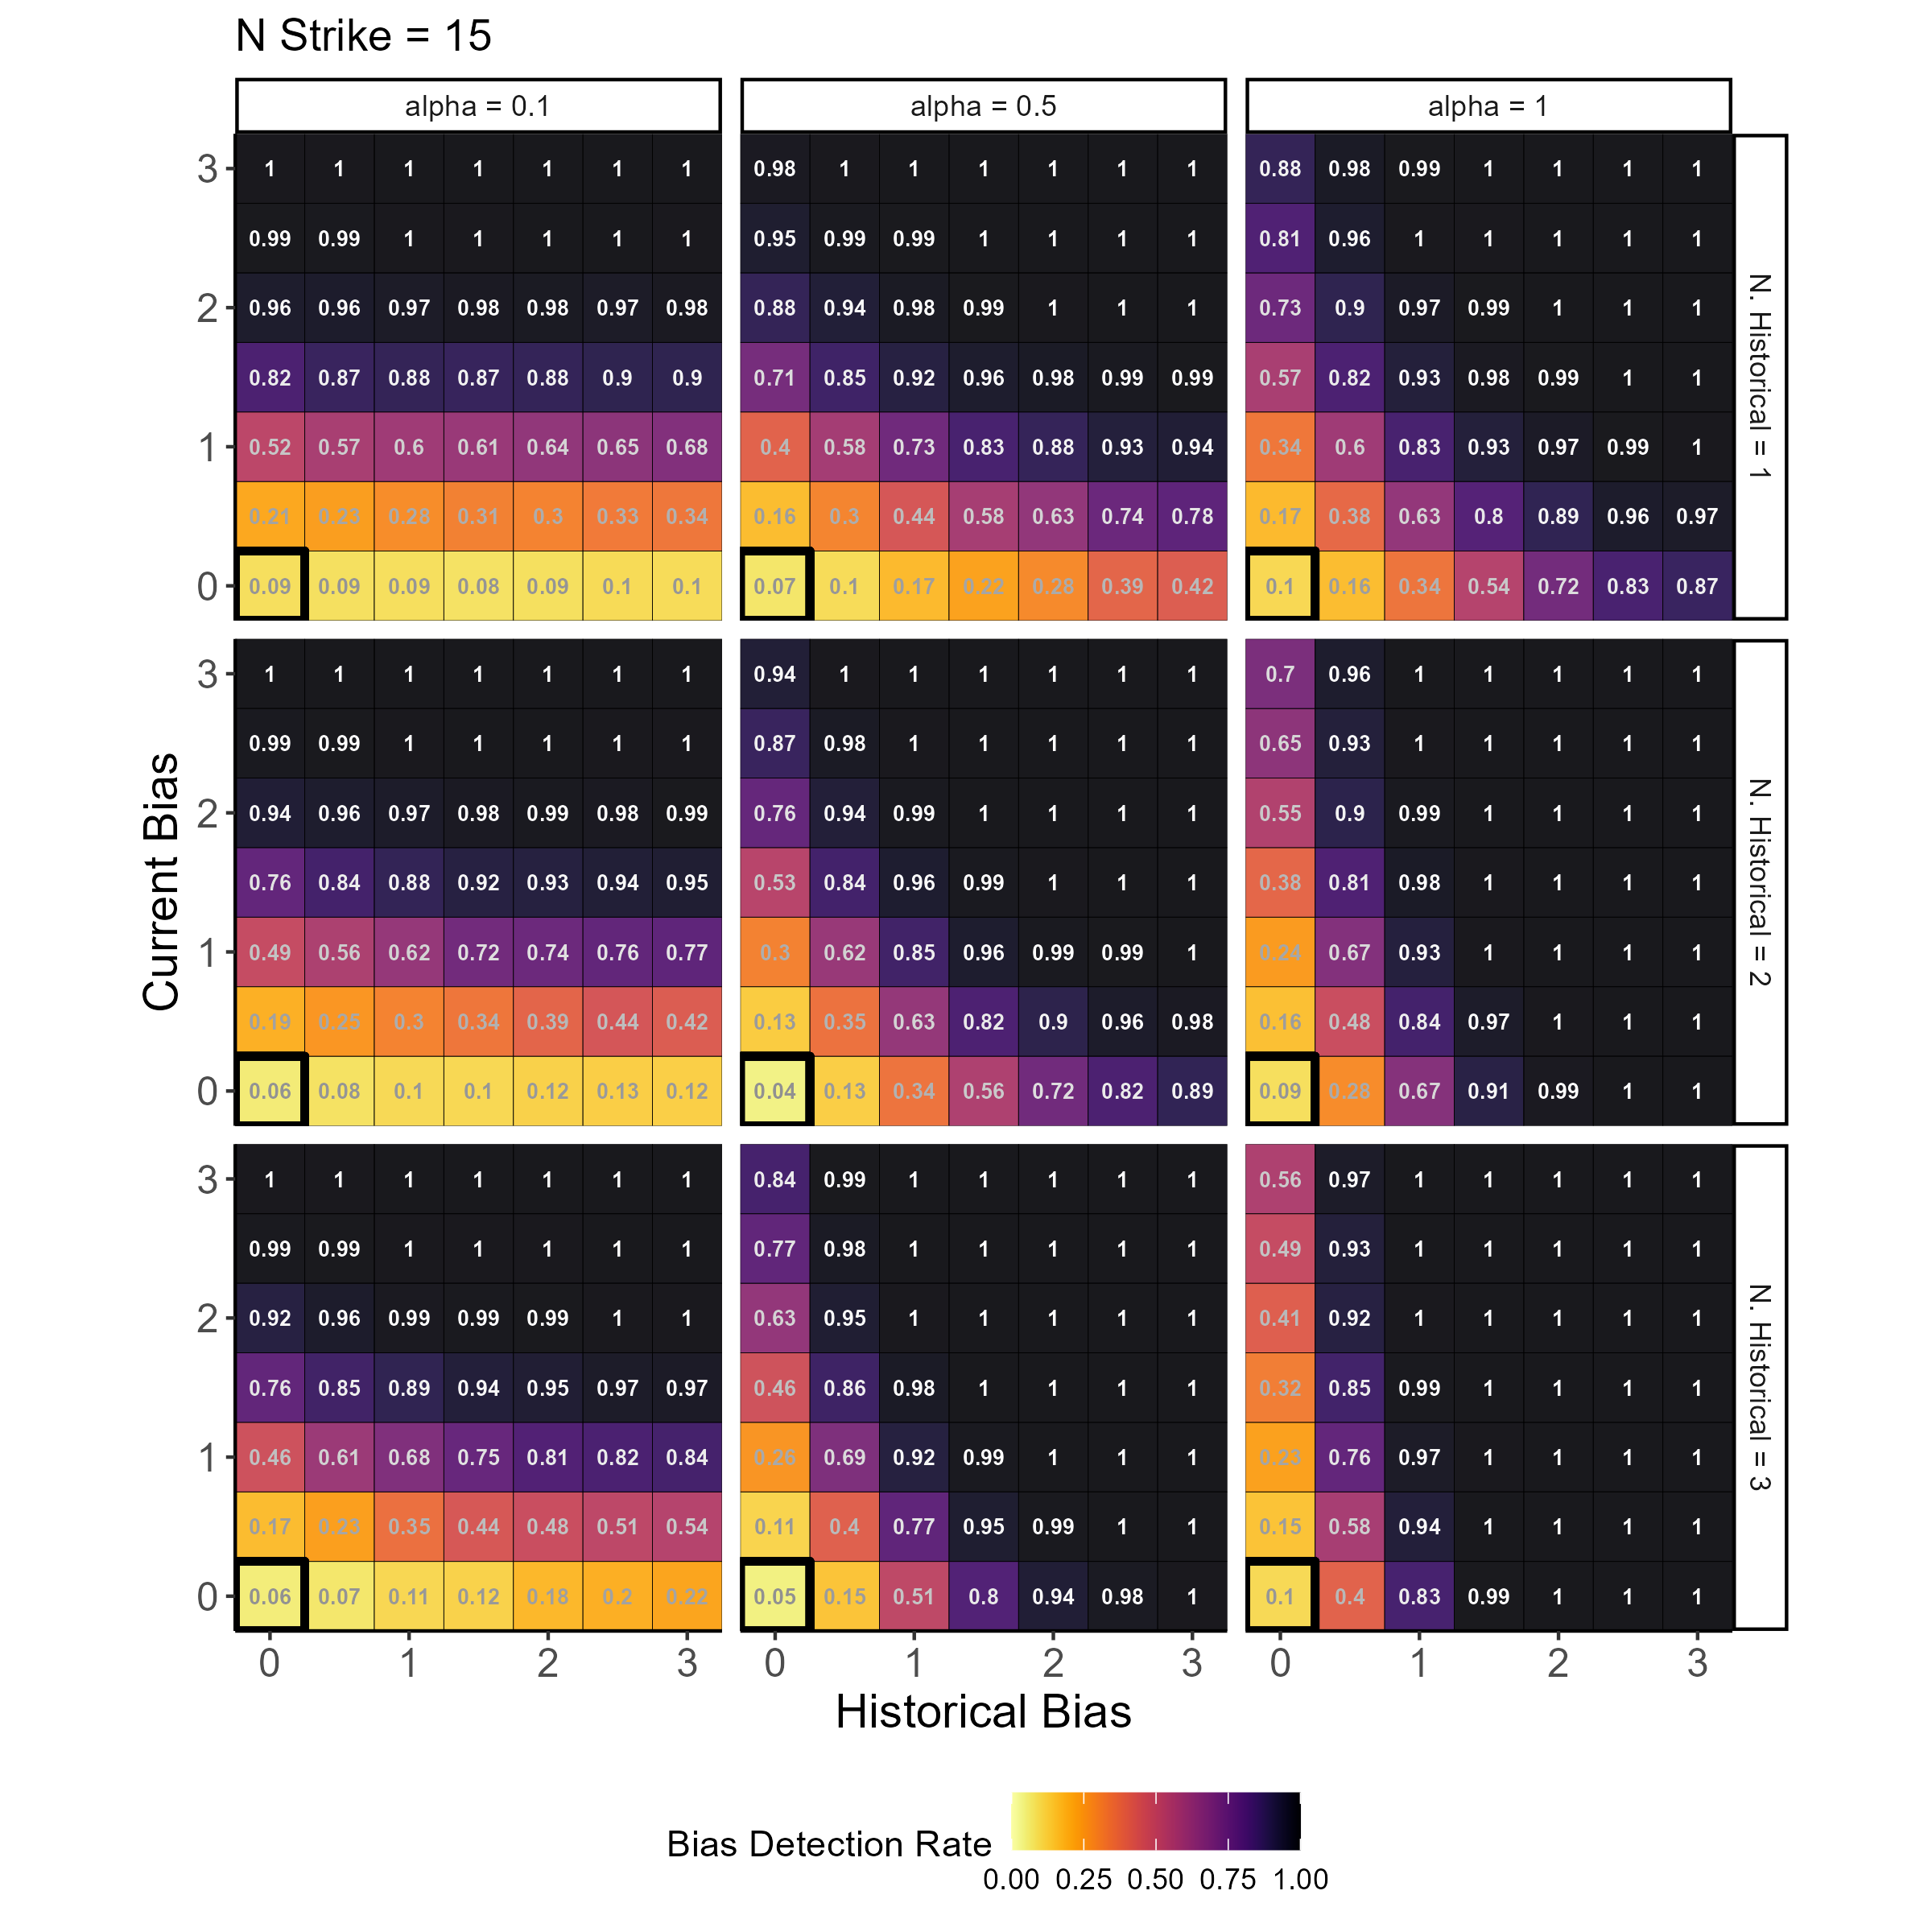
\includegraphics[width=0.95\linewidth]{../figures/pp15_90CI} 

}

\caption{Bias Detection Rates, 90 pct credible interval, 15 strike scenario}\label{fig:figbd9015}
\end{figure}

\begin{figure}

{\centering 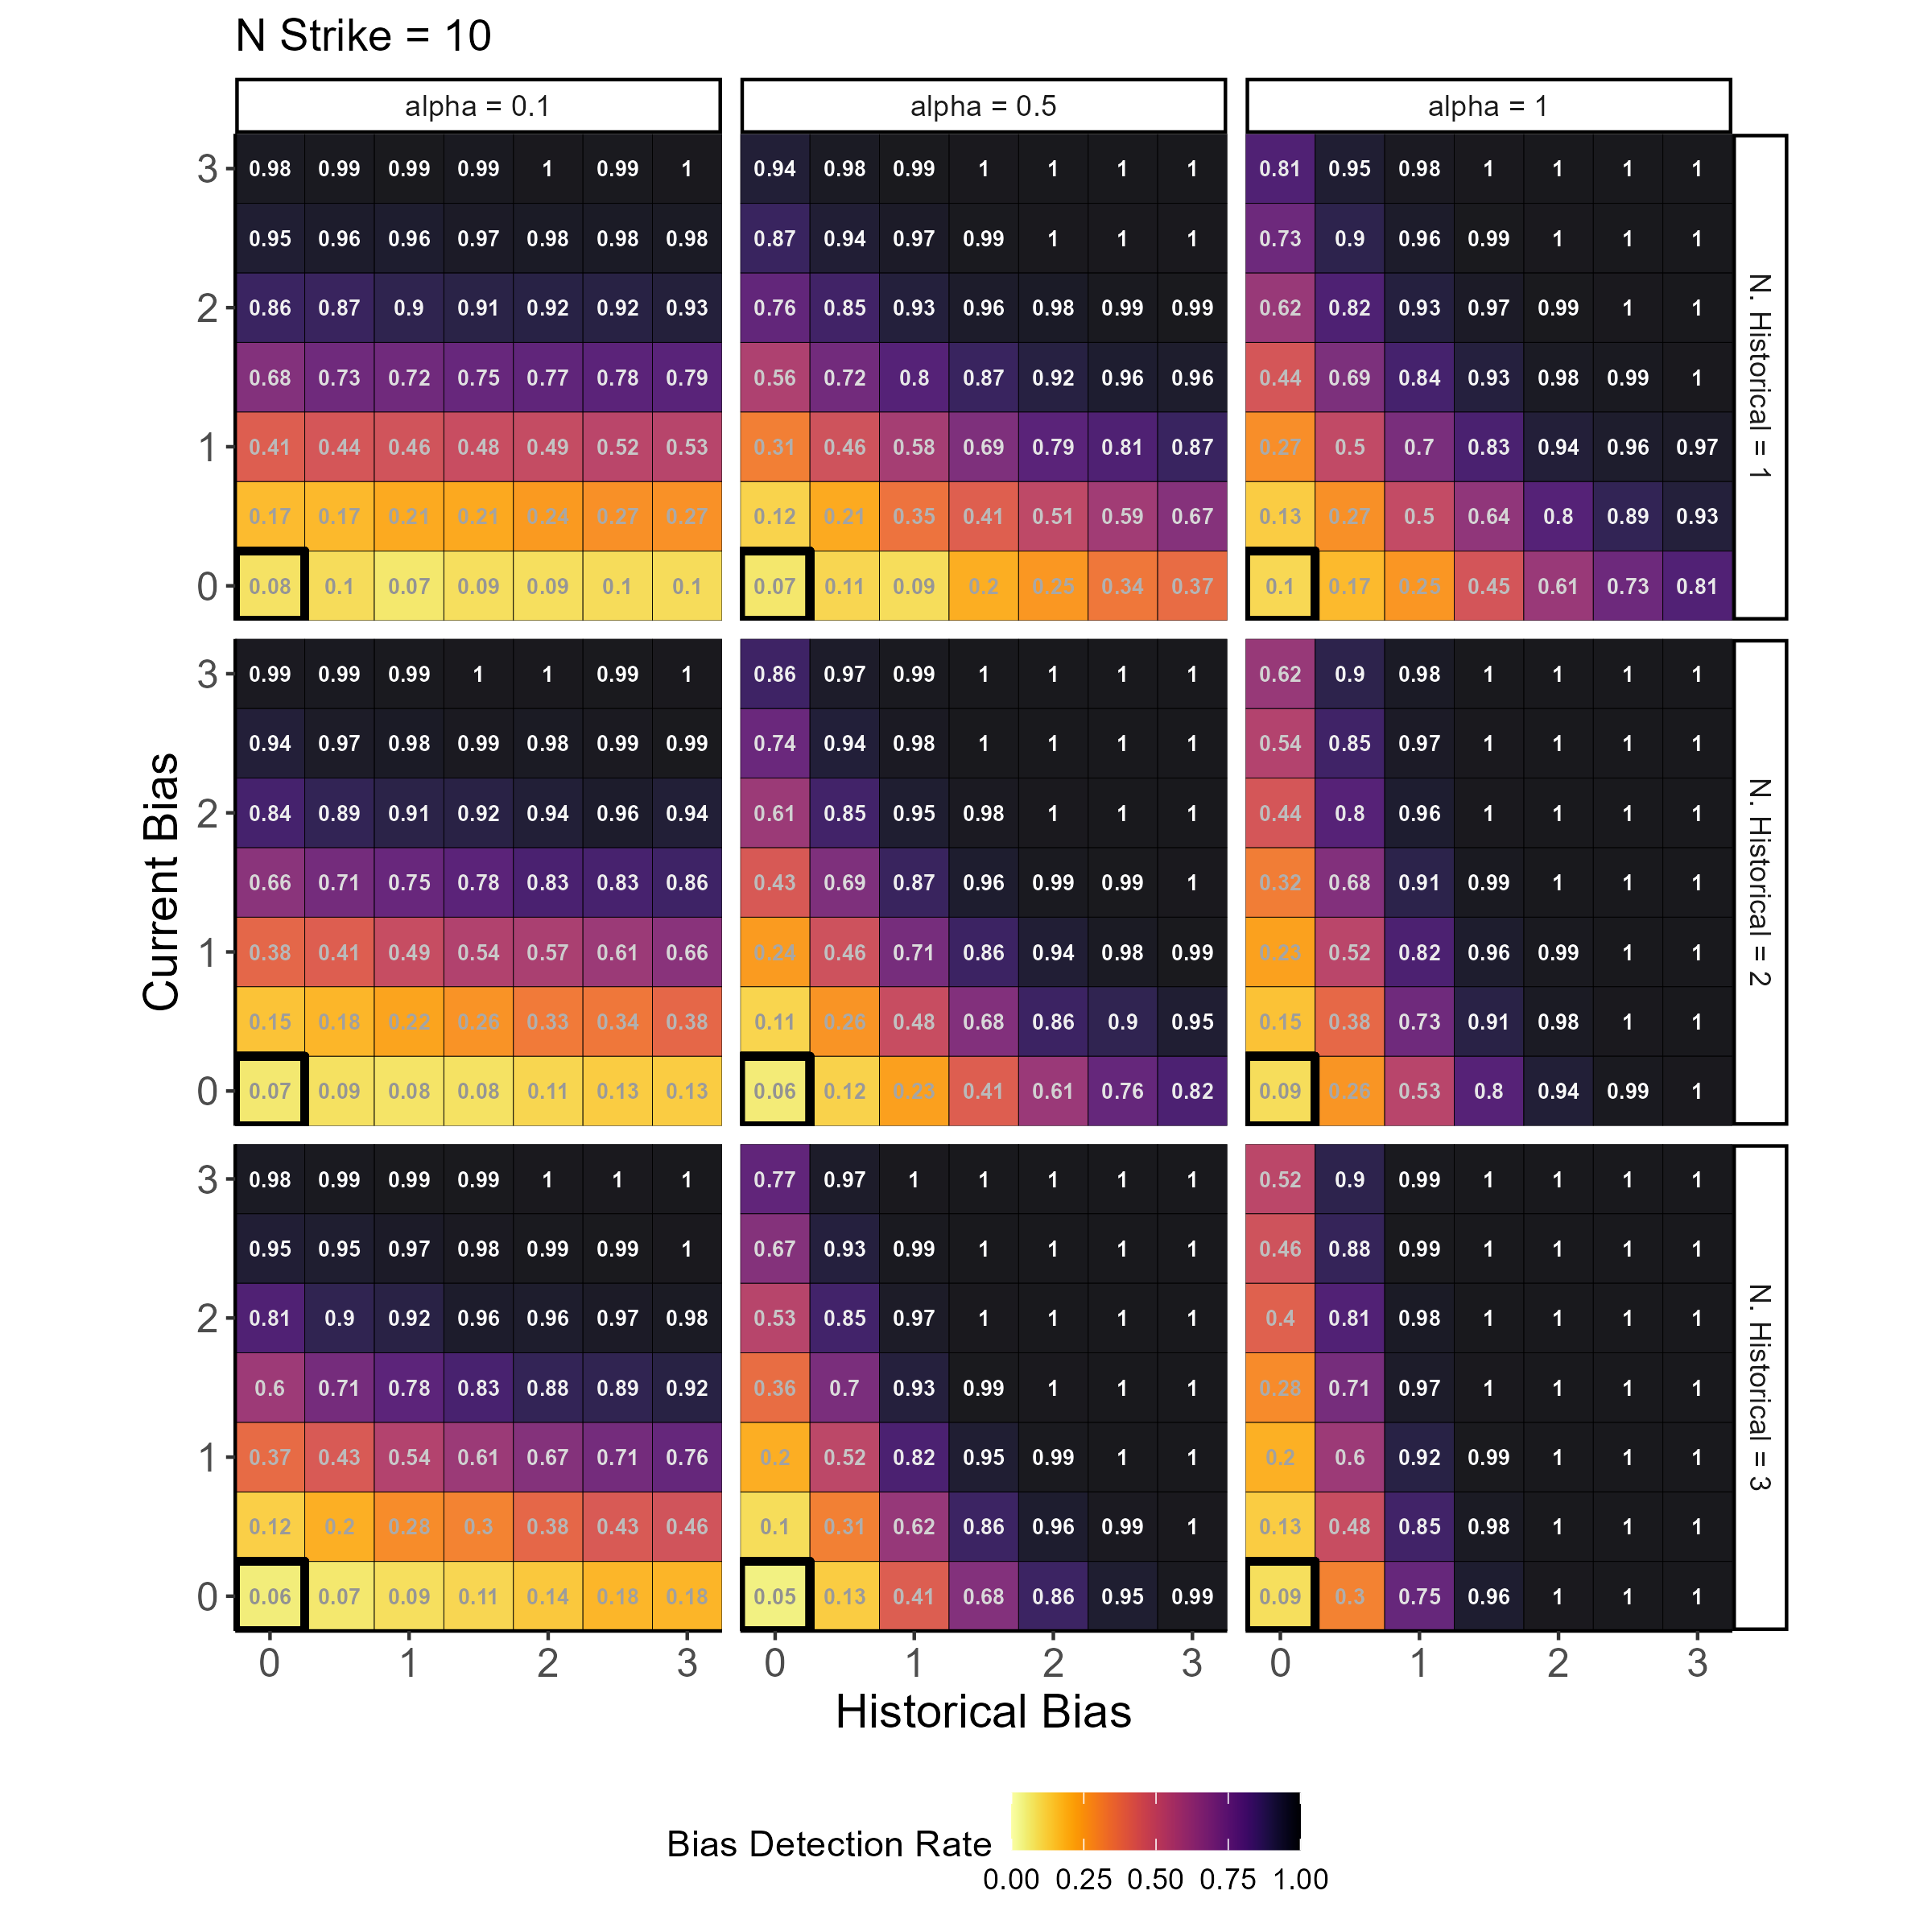
\includegraphics[width=0.95\linewidth]{../figures/pp10_90CI} 

}

\caption{Bias Detection Rates (90 pct credible interval, 10 strikes scenario)}\label{fig:figbd9010}
\end{figure}

\begin{figure}

{\centering 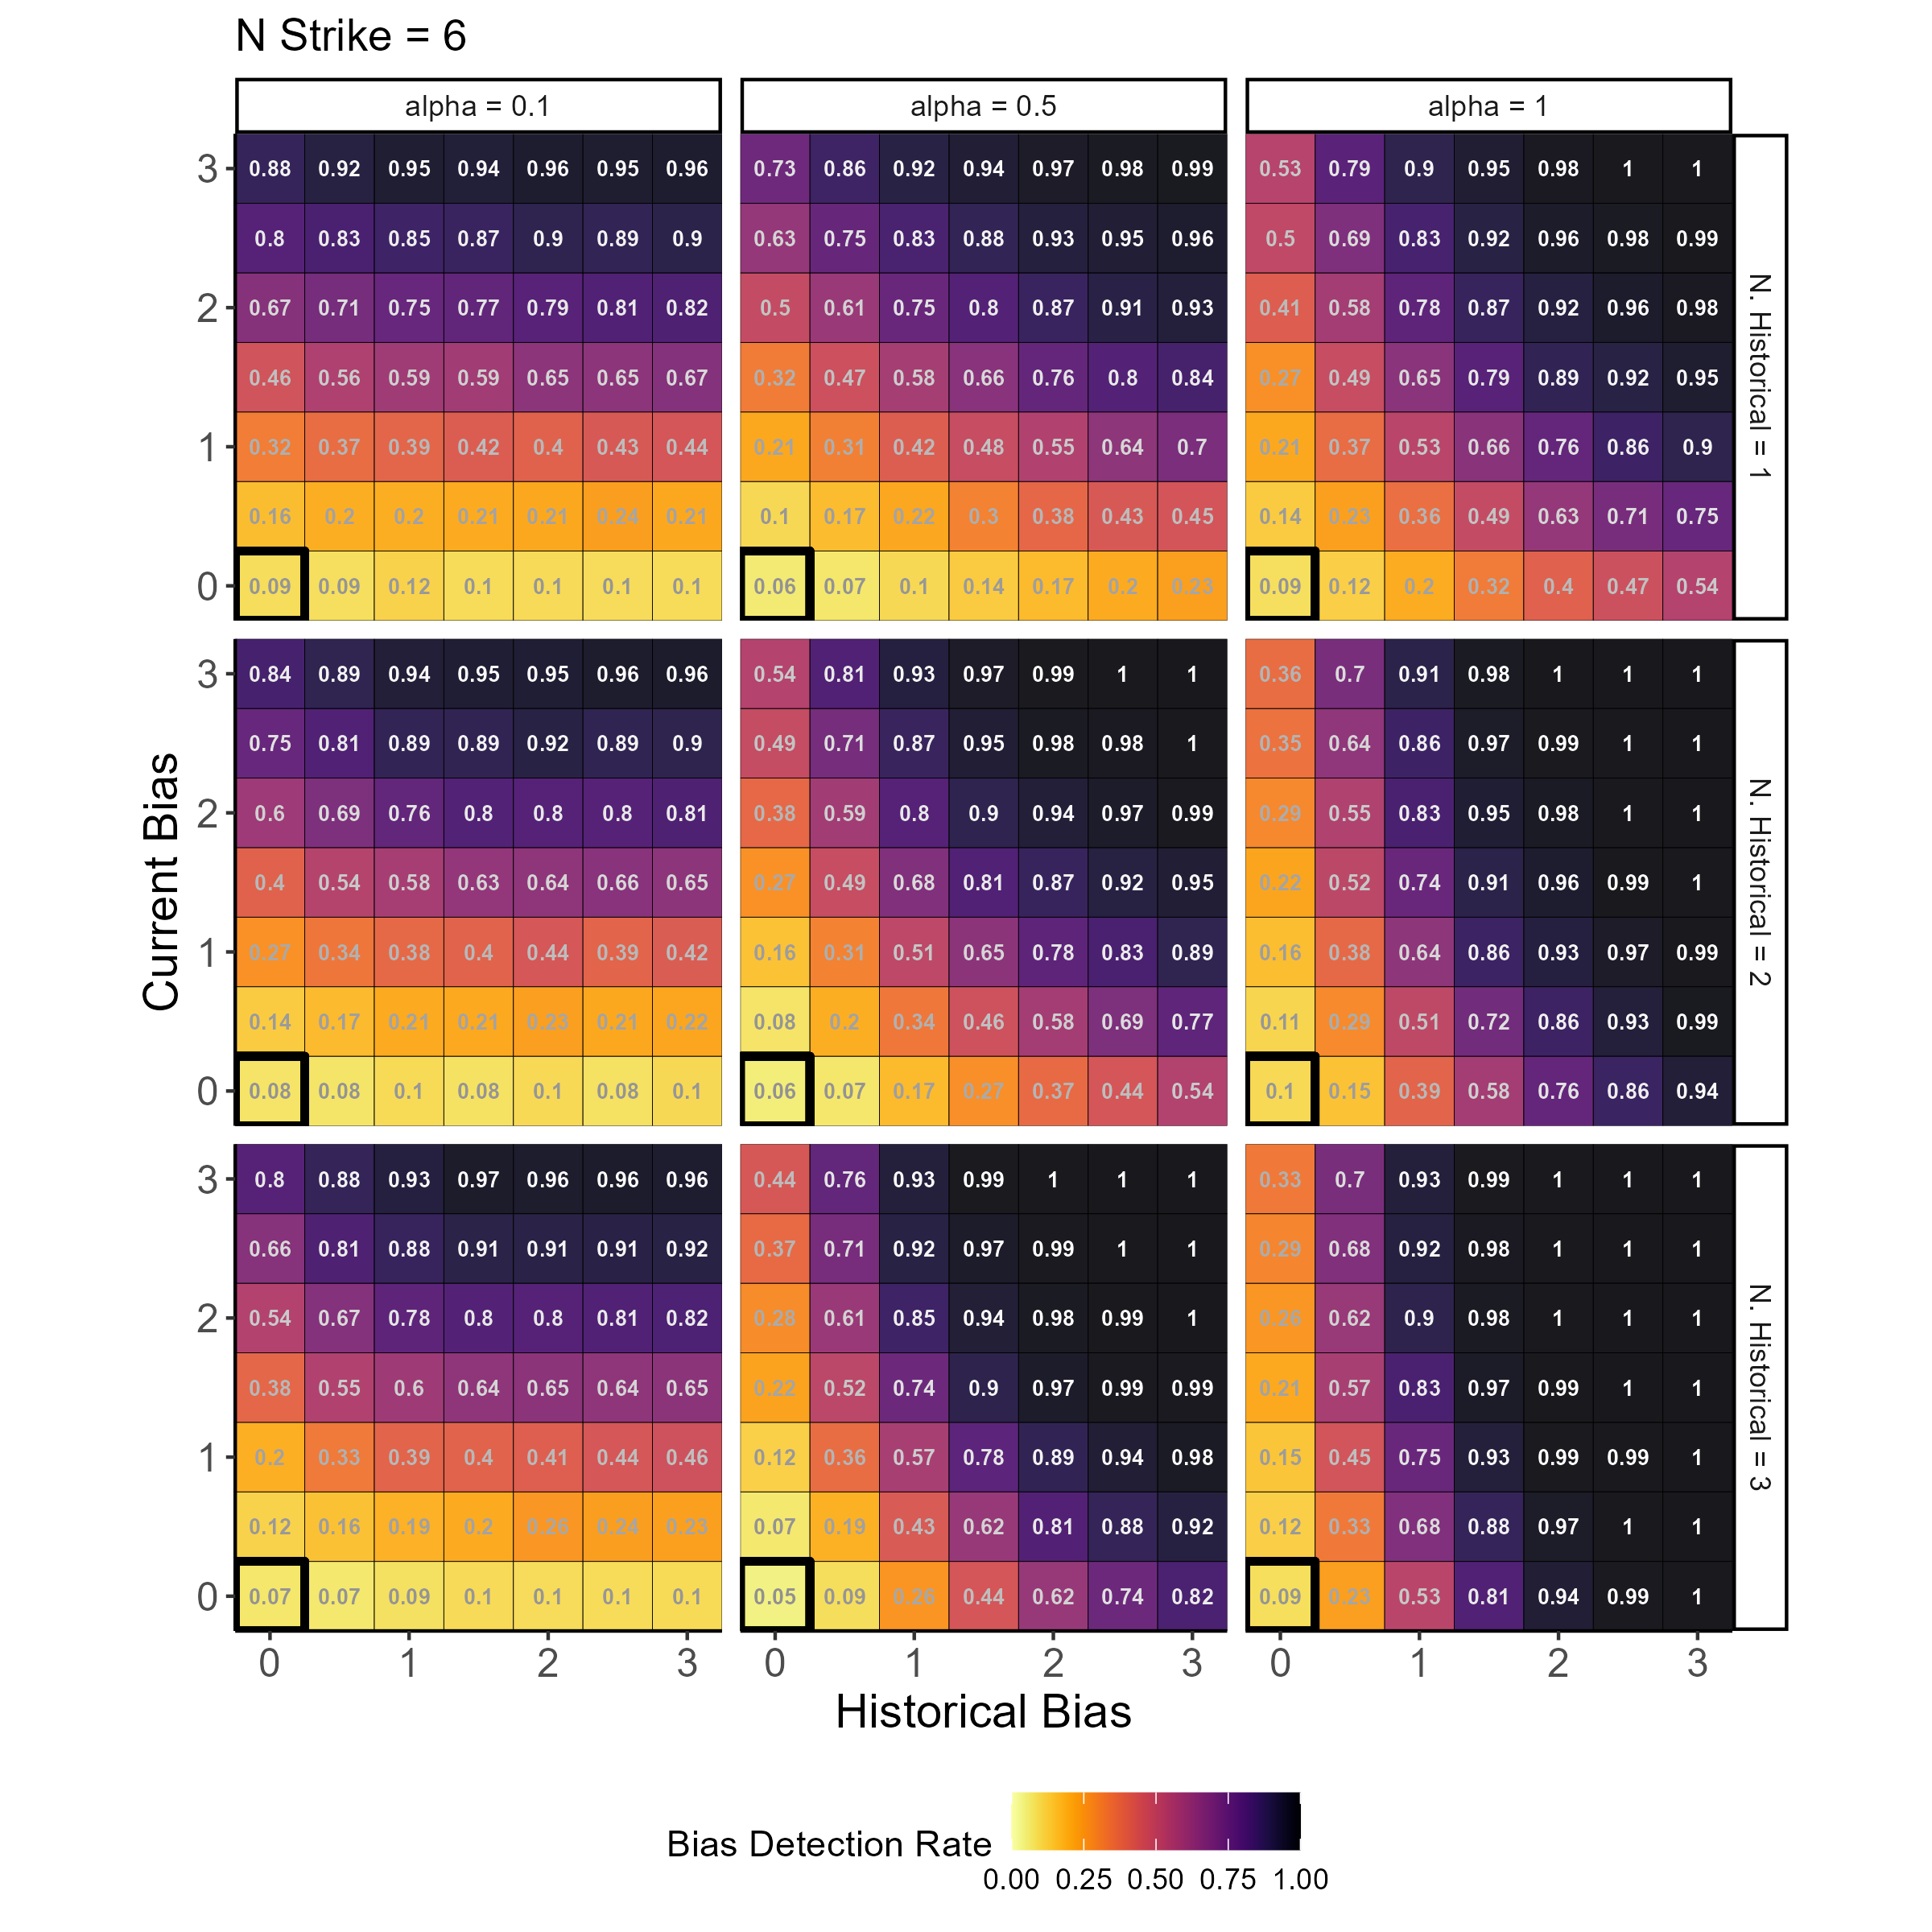
\includegraphics[width=0.95\linewidth]{../figures/pp6_90CI} 

}

\caption{Bias Detection Rates based on 90 pct credible interval for 6 strike scenario}\label{fig:figbd906}
\end{figure}

\begin{figure}

{\centering 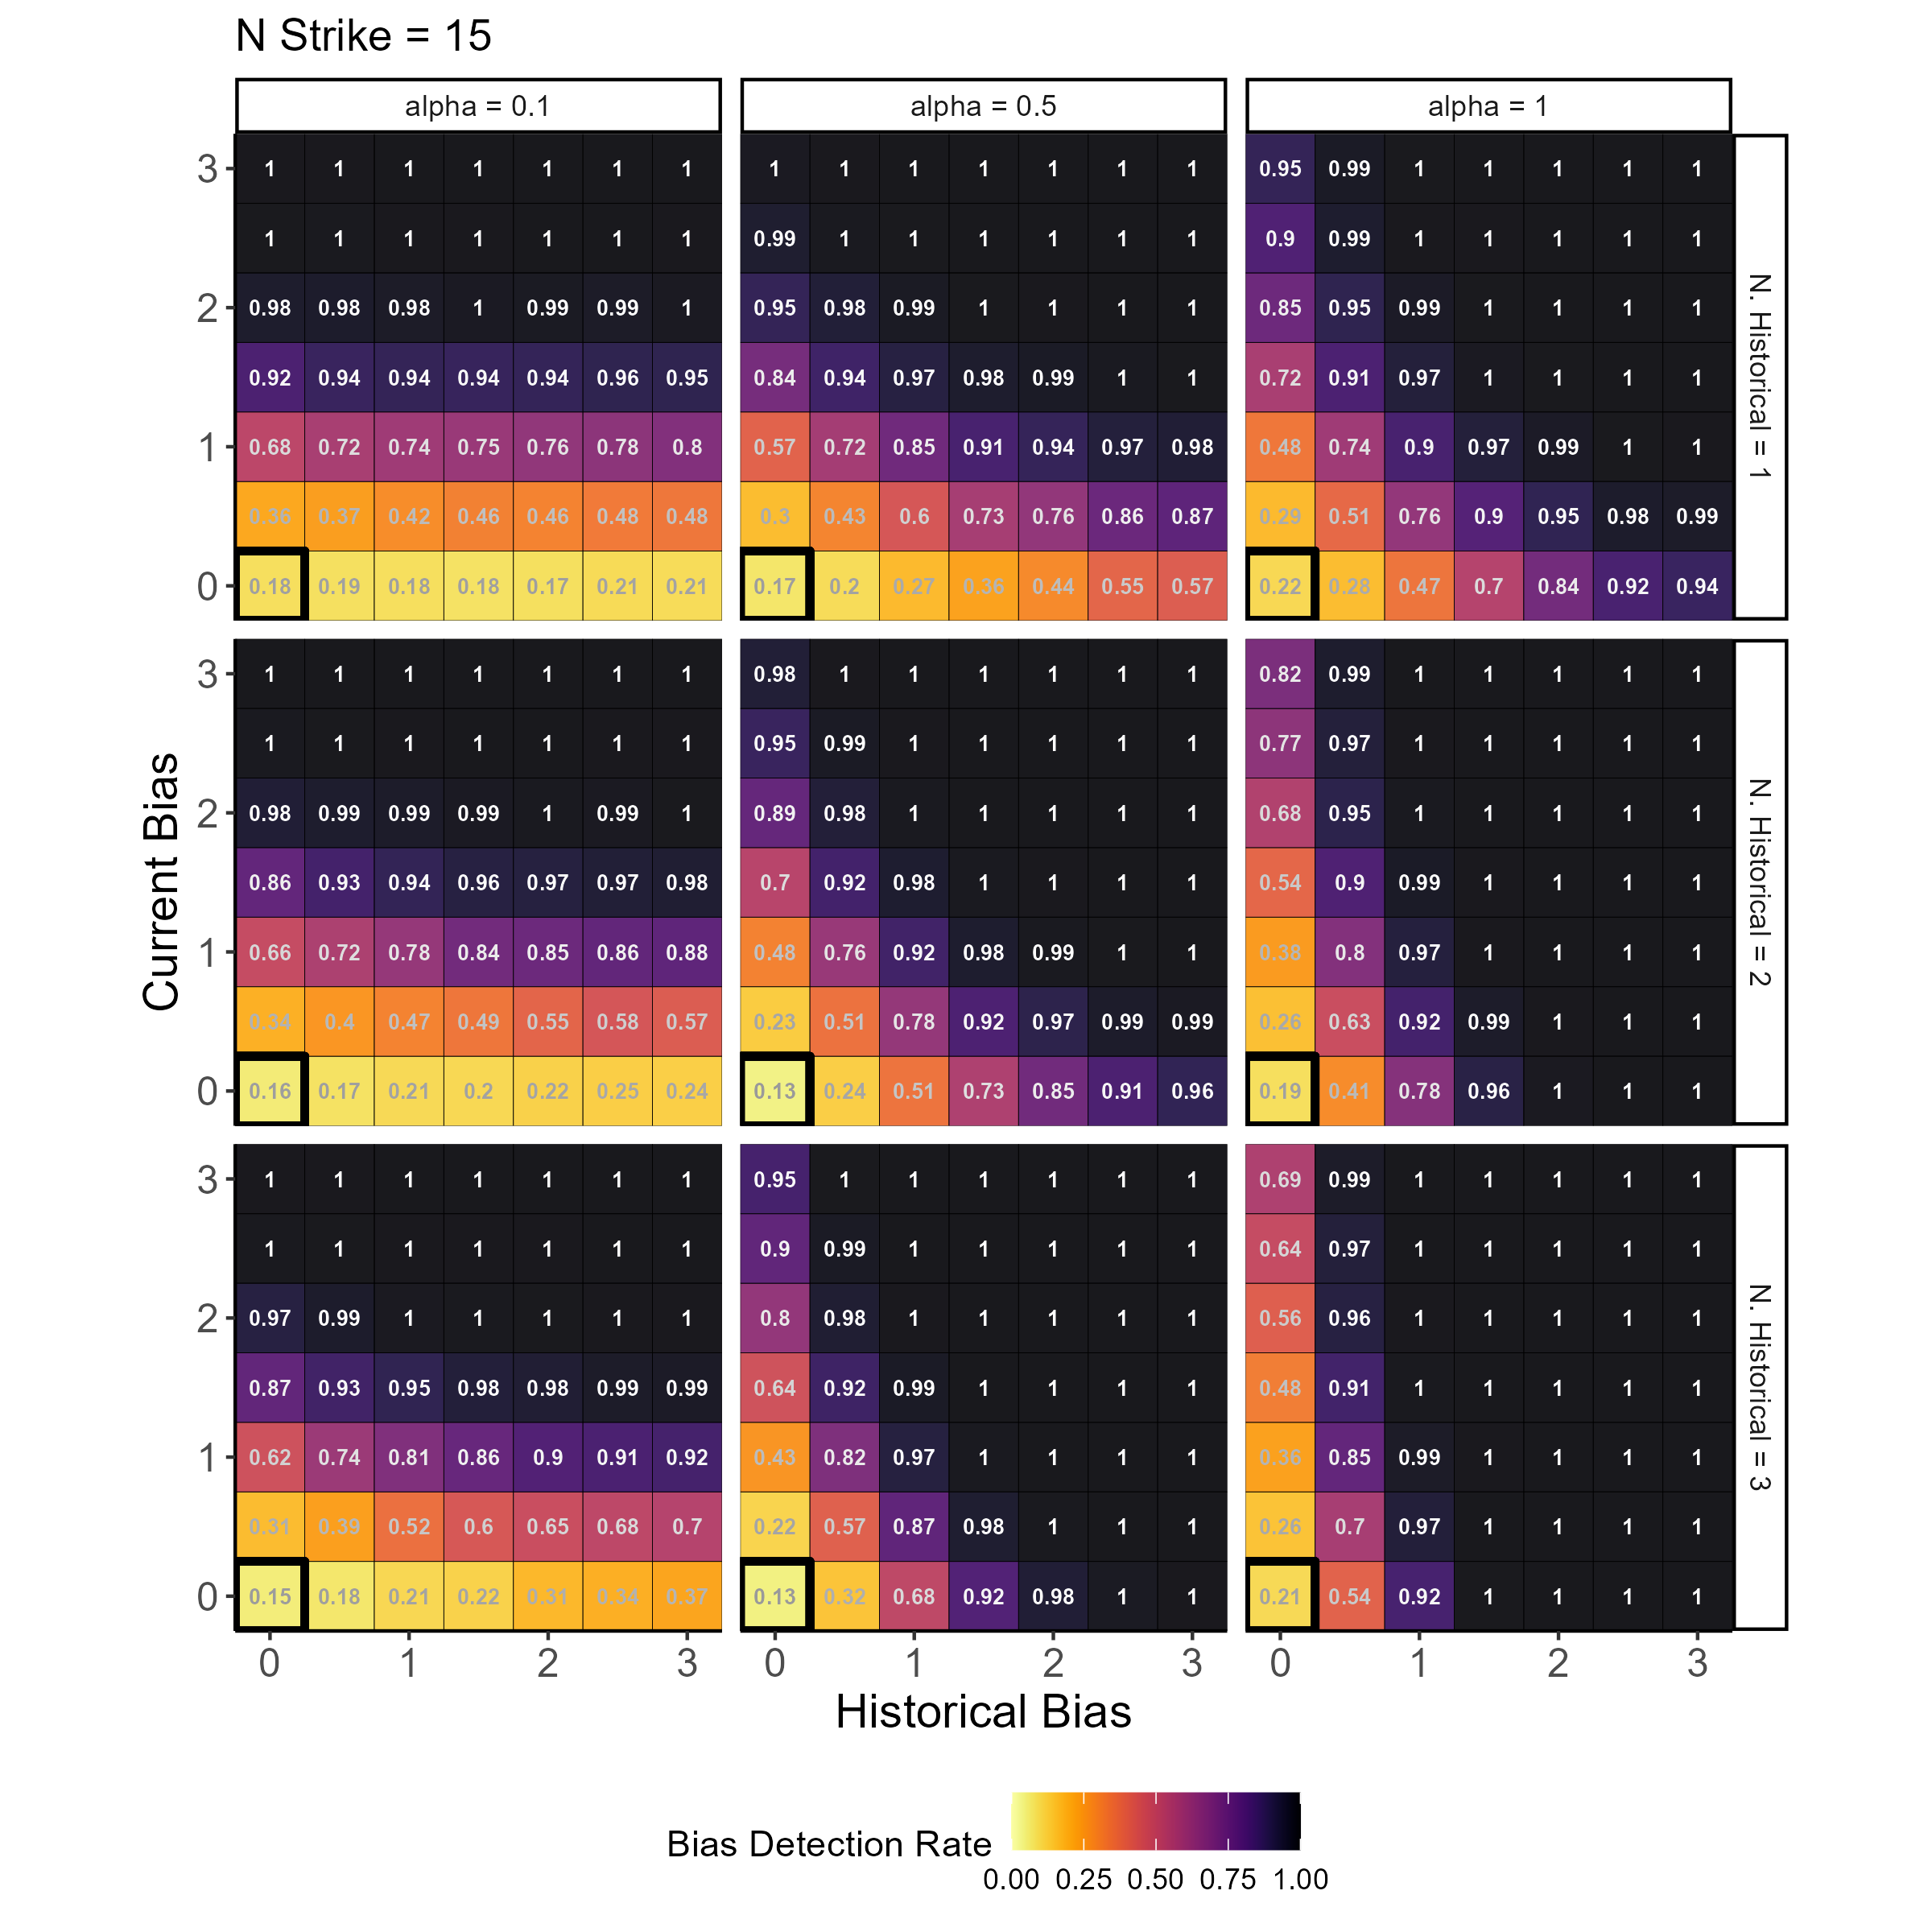
\includegraphics[width=0.95\linewidth]{../figures/pp15_80CI} 

}

\caption{Bias Detection Rates, 80 pct credible interval, 15 strike scenario}\label{fig:figbd8015}
\end{figure}

\begin{figure}

{\centering 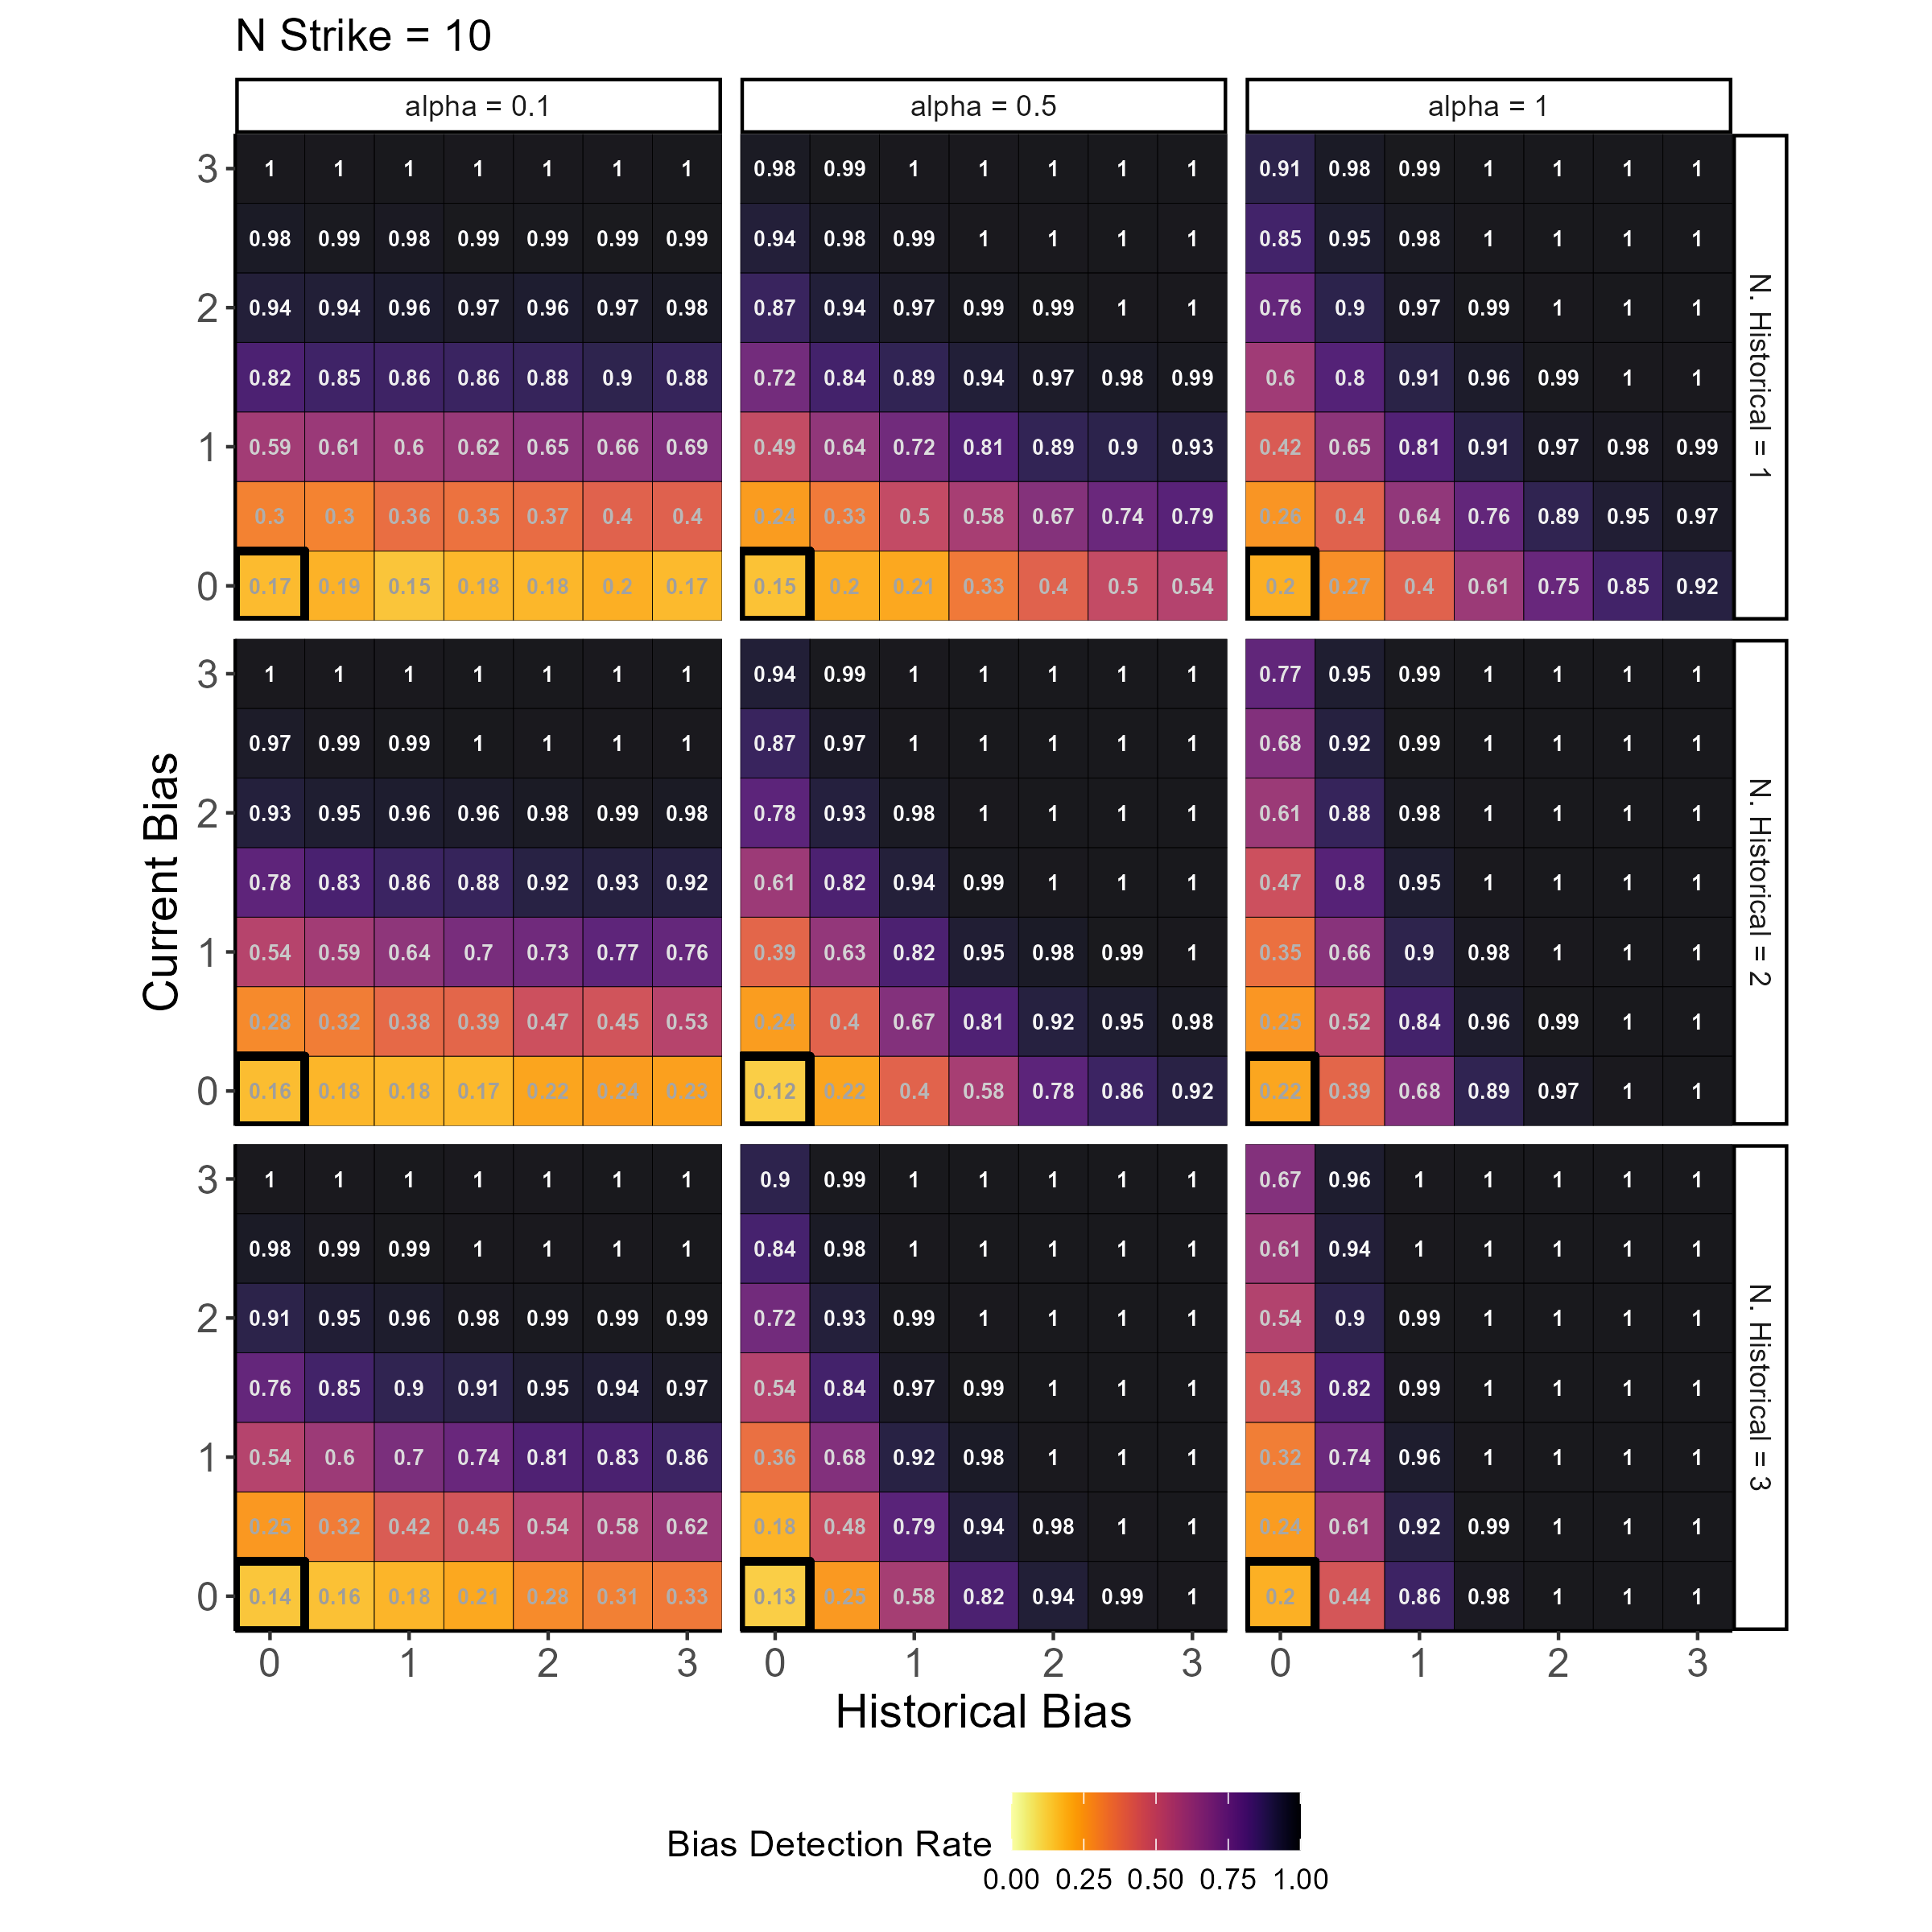
\includegraphics[width=0.95\linewidth]{../figures/pp10_80CI} 

}

\caption{Bias Detection Rates (80 pct credible interval, 10 strikes scenario)}\label{fig:figbd8010}
\end{figure}

\begin{figure}

{\centering 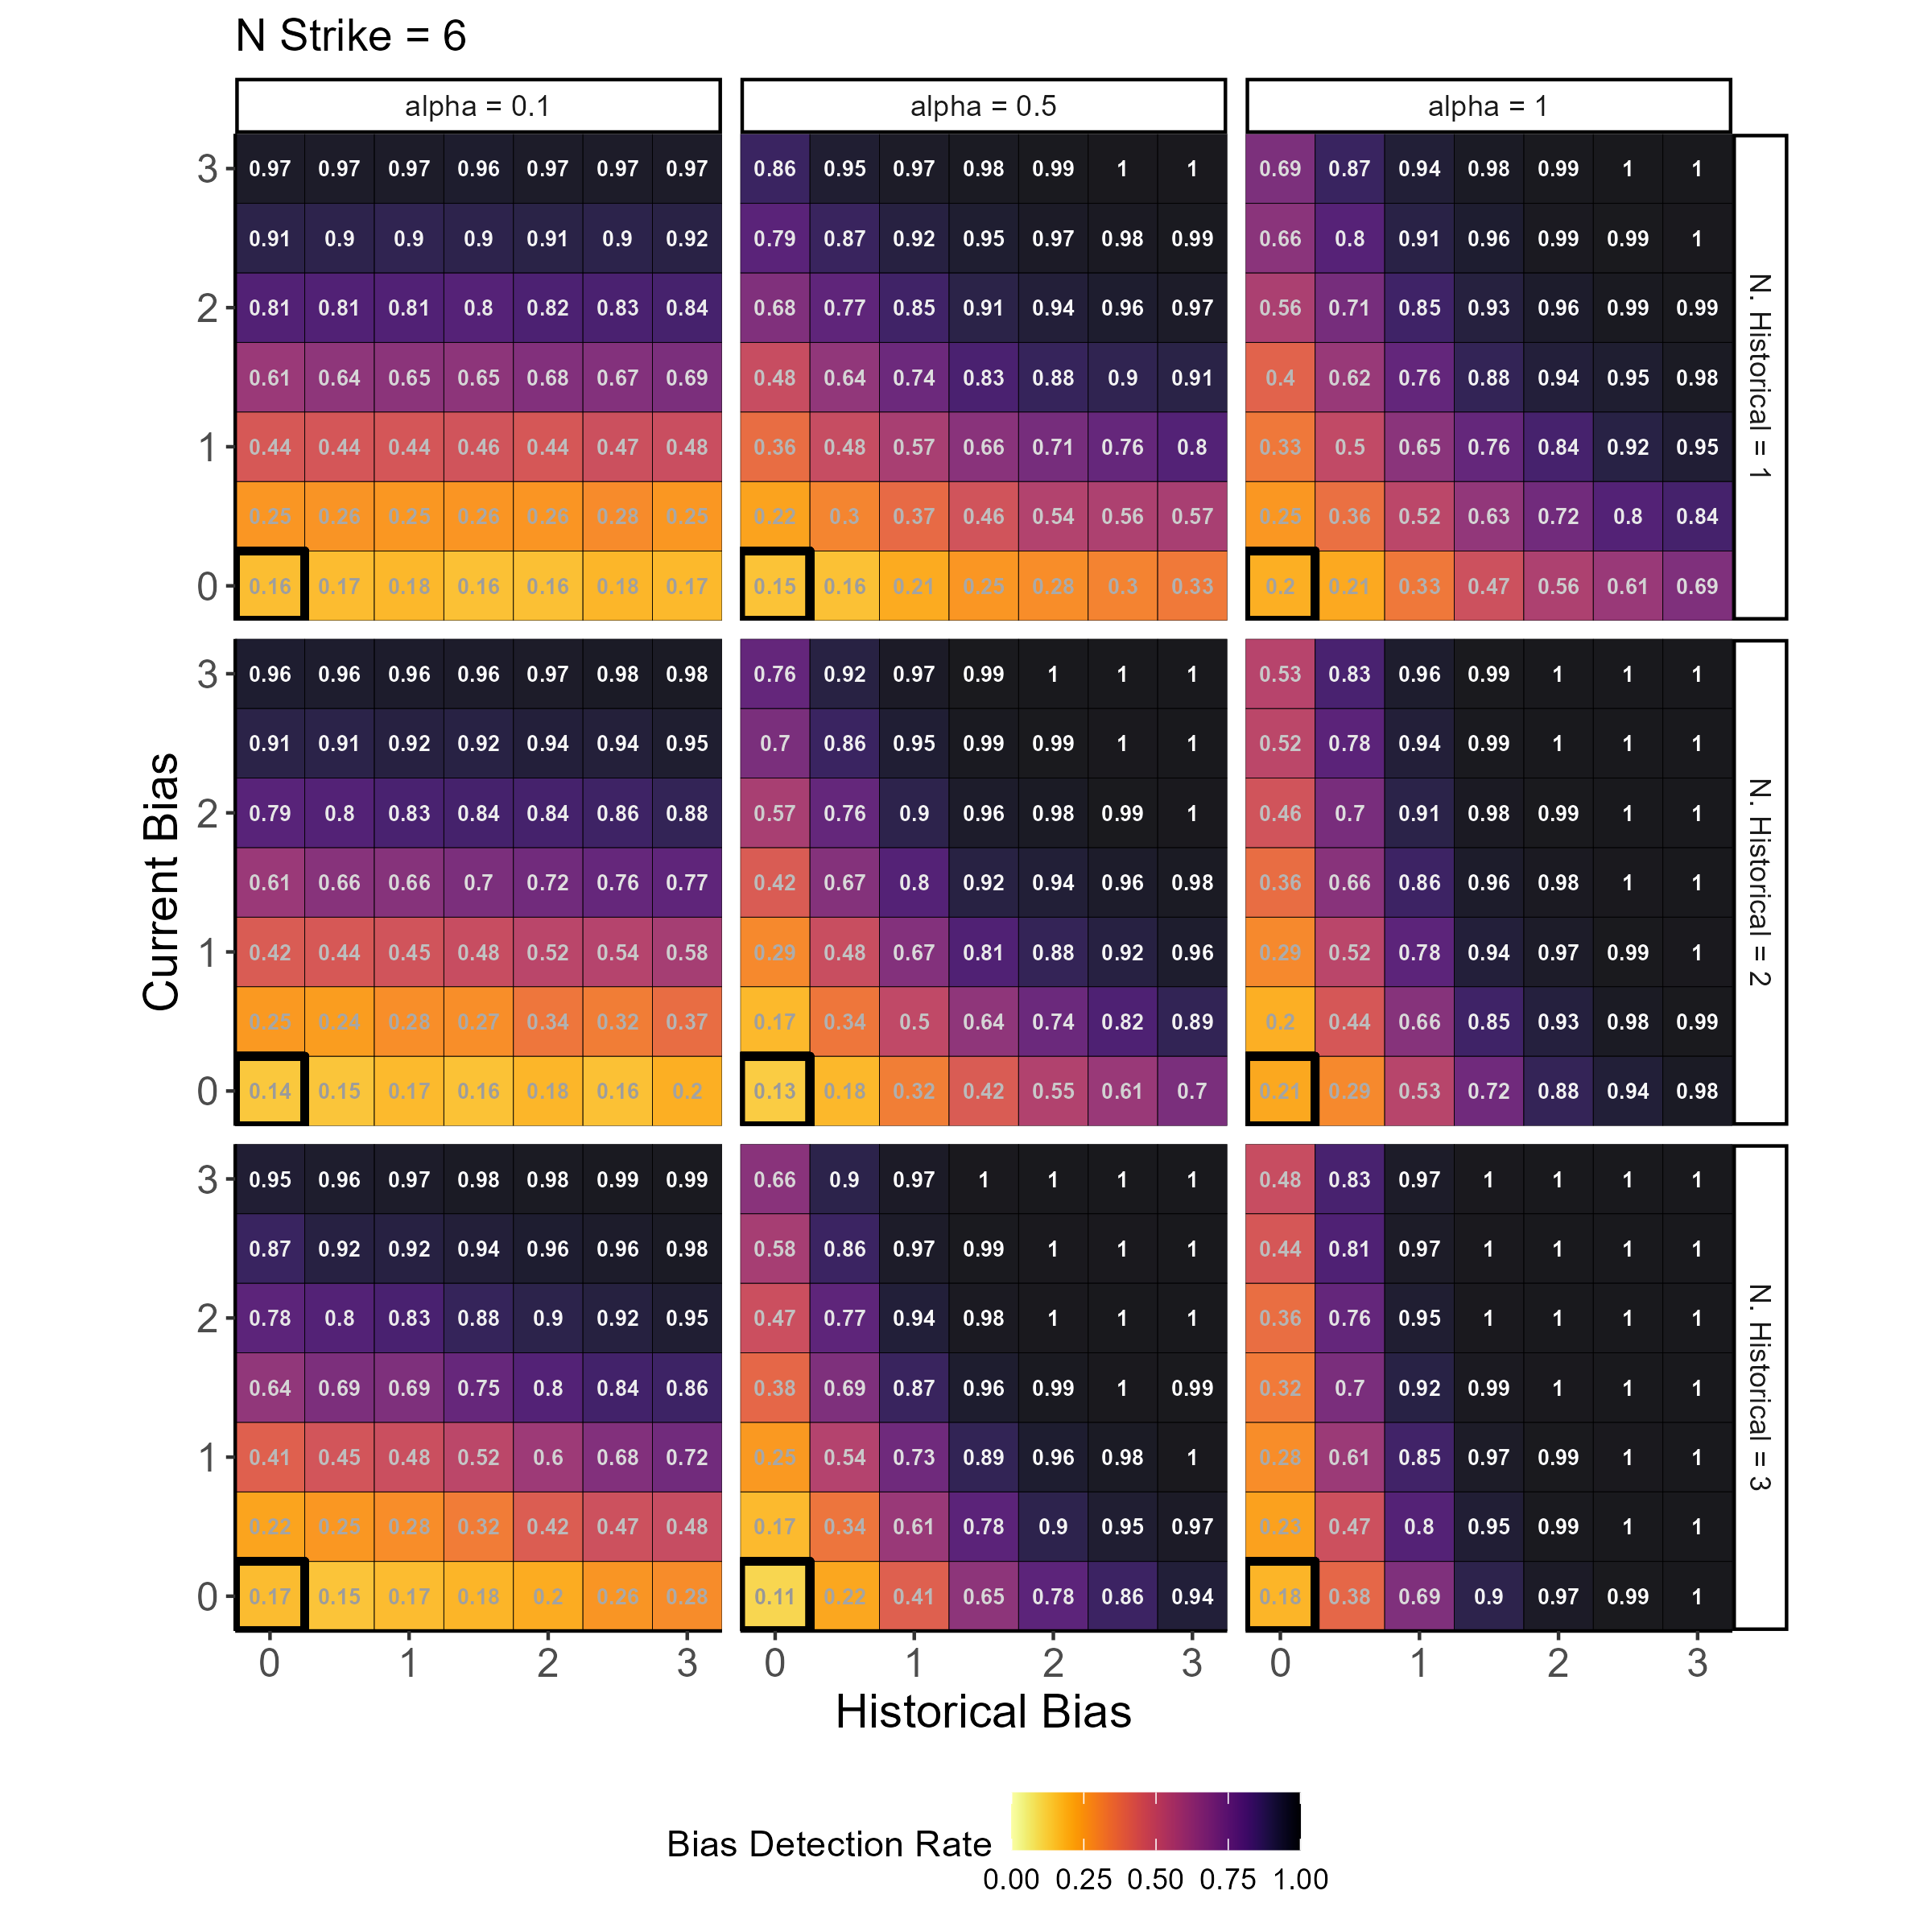
\includegraphics[width=0.95\linewidth]{../figures/pp6_80CI} 

}

\caption{Bias Detection Rates based on 80 pct credible interval for 6 strike scenario}\label{fig:figbd806}
\end{figure}

\hypertarget{prototype-software-application}{%
\subsection{Prototype Software Application}\label{prototype-software-application}}

\hypertarget{data-collection}{%
\subsubsection{Data Collection}\label{data-collection}}

To collect the historical strike data for the prototype software application, one of us filed a request with the U.S. District Court of Connecticut based on 28 U.S.C. \(\S\) 1868. Thereafter, we received copies of certain jury-selection records associated with twenty-nine criminal cases in that court during this period. These included strike sheets that indicated the identification number of prospective jurors who were struck by peremptory challenge, the order in which they were struck, and which side (prosecutor or defense) struck which juror. Such records also included a tally of answers to juror questionnaires that asked each prospective juror to report their race and gender.

These records, however, often did not indicate the identity of the attorneys exercising the strikes. While the standard forms included a signature line for the attorney, many were left blank or filled with illegible signatures. Accordingly, we turned to the publicly-available docket sheets for each case for the names of the lawyers who appeared in the case on behalf of the prosecution (the United States Attorney's office) or the criminal defendant(s) on the date(s) of jury selection. Where only a single attorney represented a party during jury selection, it was easy to attribute the pattern of strikes to that attorney. Where multiple lawyers appeared for one side, we attributed to each of them that side's pattern of peremptory challenges in that case. In such cases, neither the jury-selection documents nor the docket sheets indicated any hierarchy among multiple lawyers or any other basis to attribute strikes to only one attorney among them. After generating a dataset based on these documents, we kept only strikes where a criminal defendant was represented by an attorney. Finally, to de-identify this dataset, we excluded defendant names and substituted fictitious names for the attorneys using the charlatan package (Chamberlain and Voytovich 2020).

\hypertarget{additional-illustrations}{%
\subsubsection{Additional Illustrations}\label{additional-illustrations}}

Suppose the same scenario discussed in section \ref{prototype}, except now the strike tally indicates the pattern of strikes by these attorneys against female prospective jurors. If so, we select ``gender'' as the cognizable class, and the density plots update accordingly (Figure \ref{fig:figapp3}(left)).

\begin{figure}
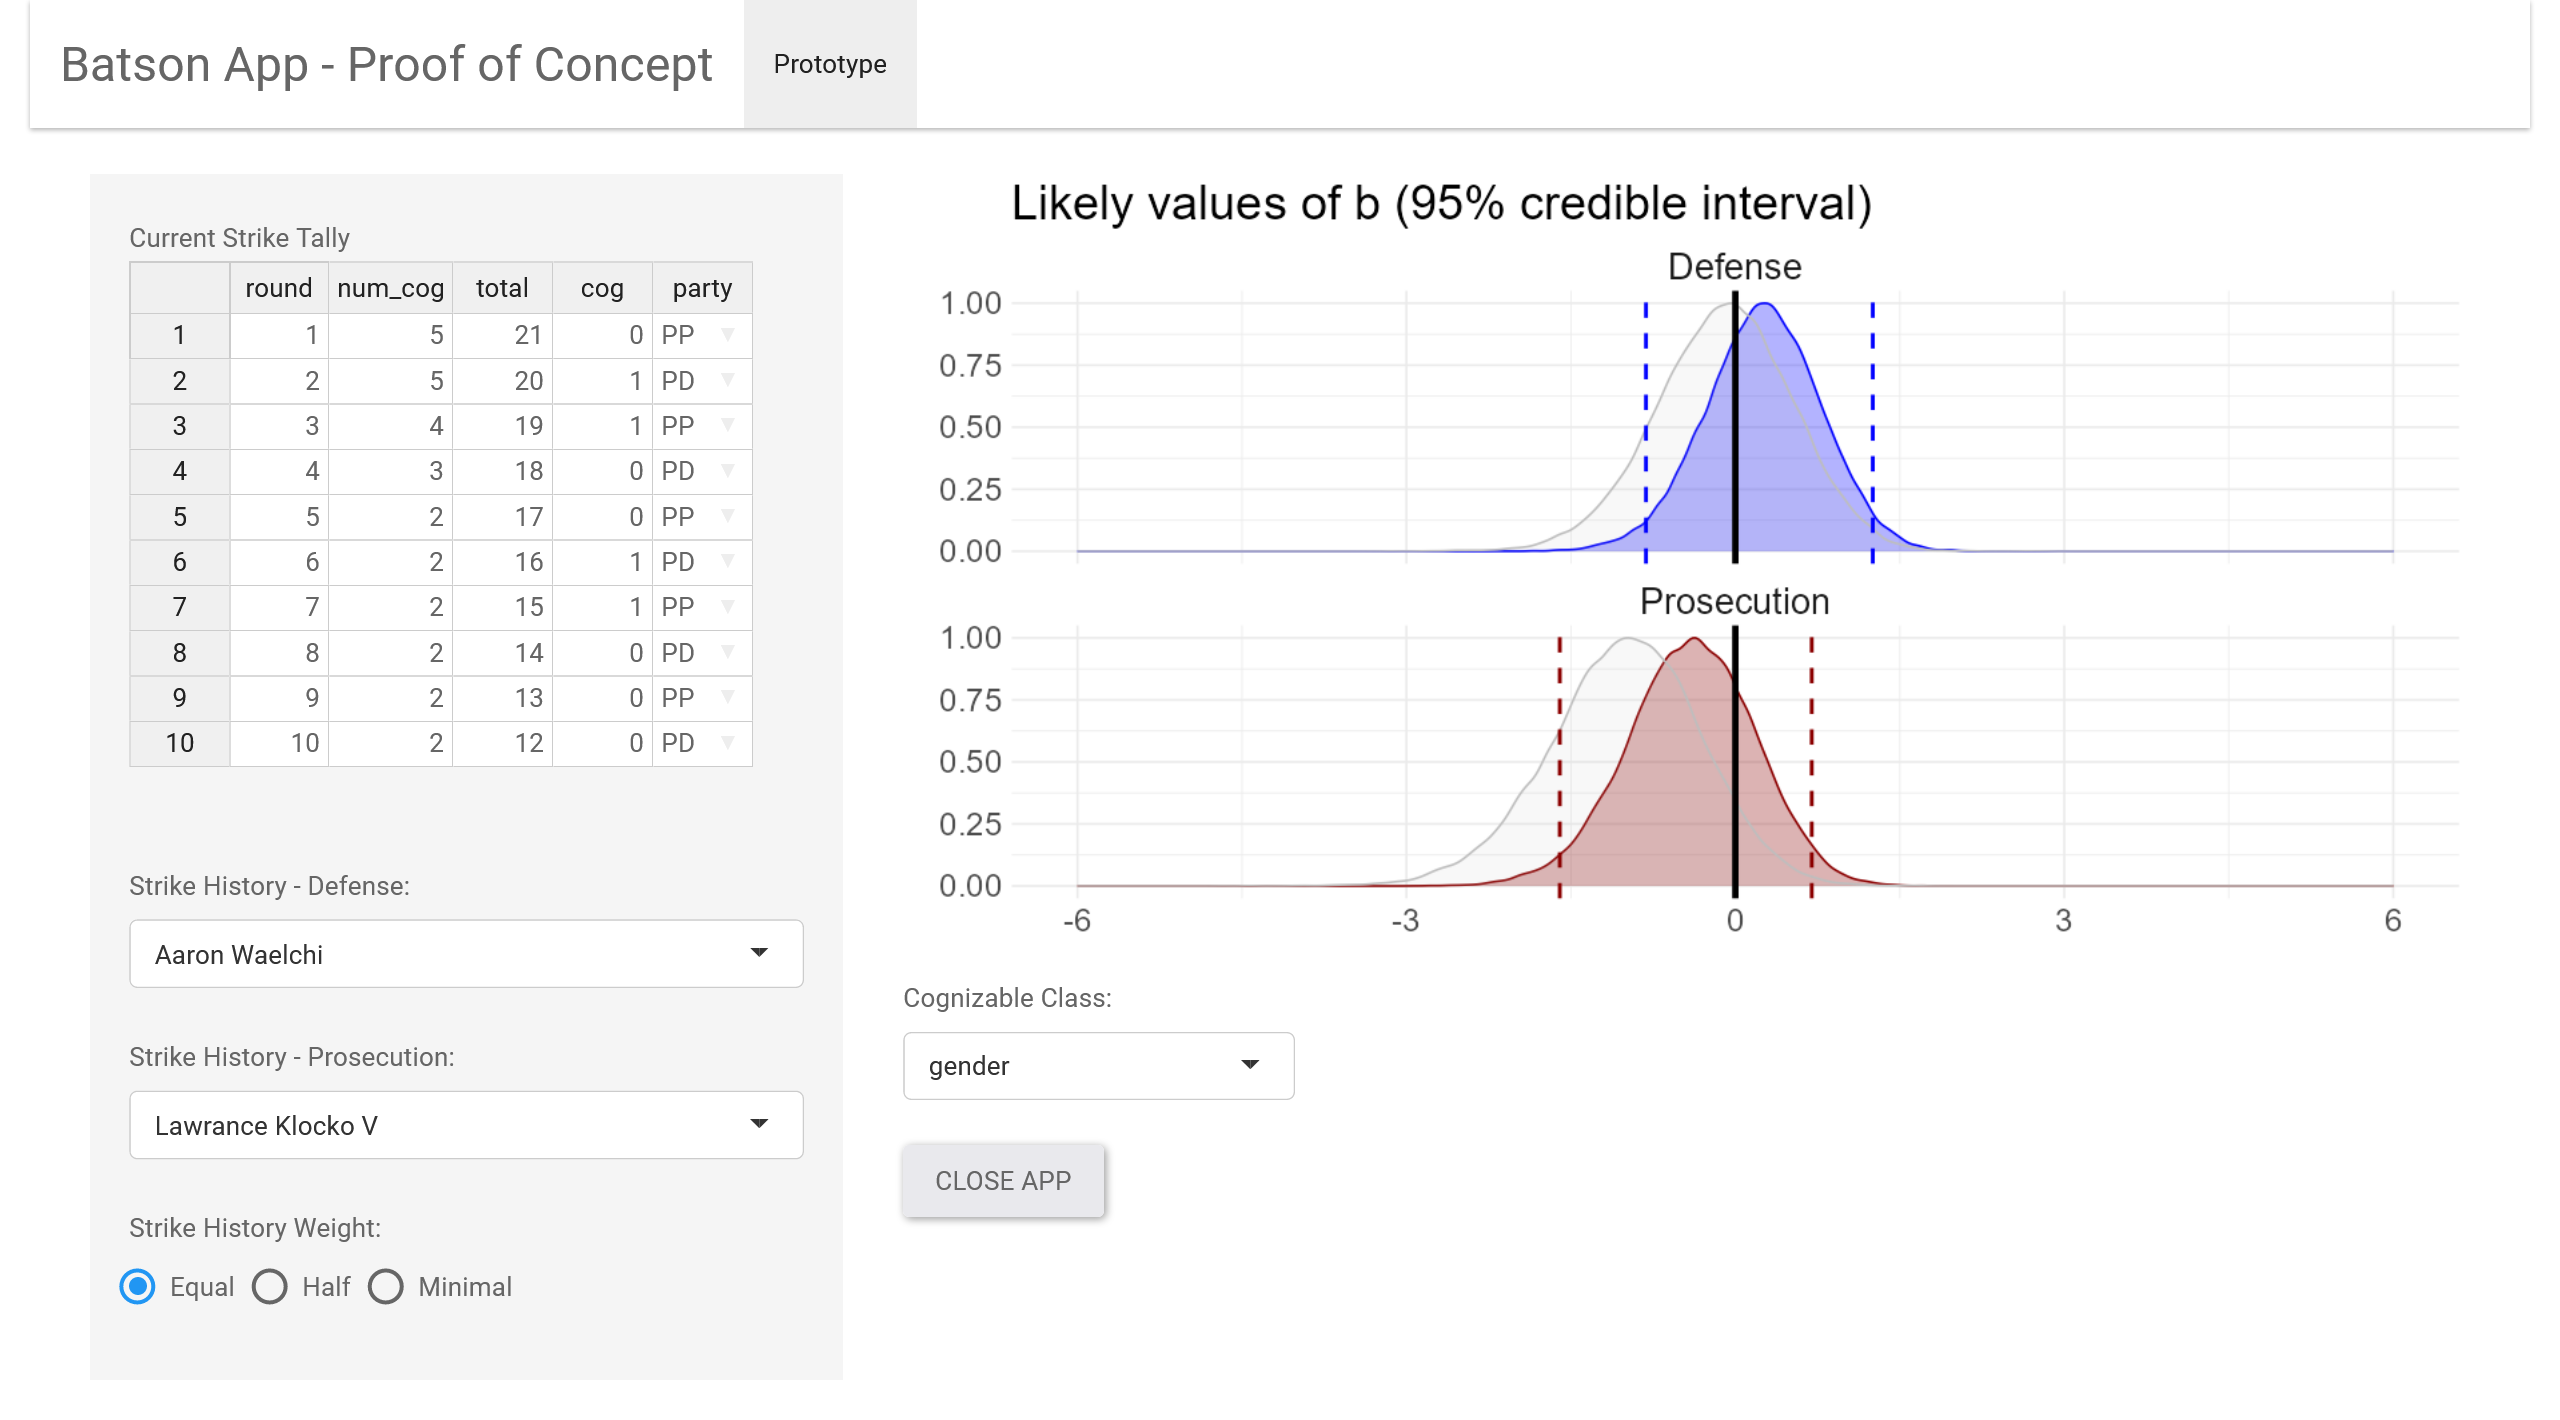
\includegraphics[width=0.5\linewidth]{../figures/batson_app_screenshots/batson_app_screenshot3} 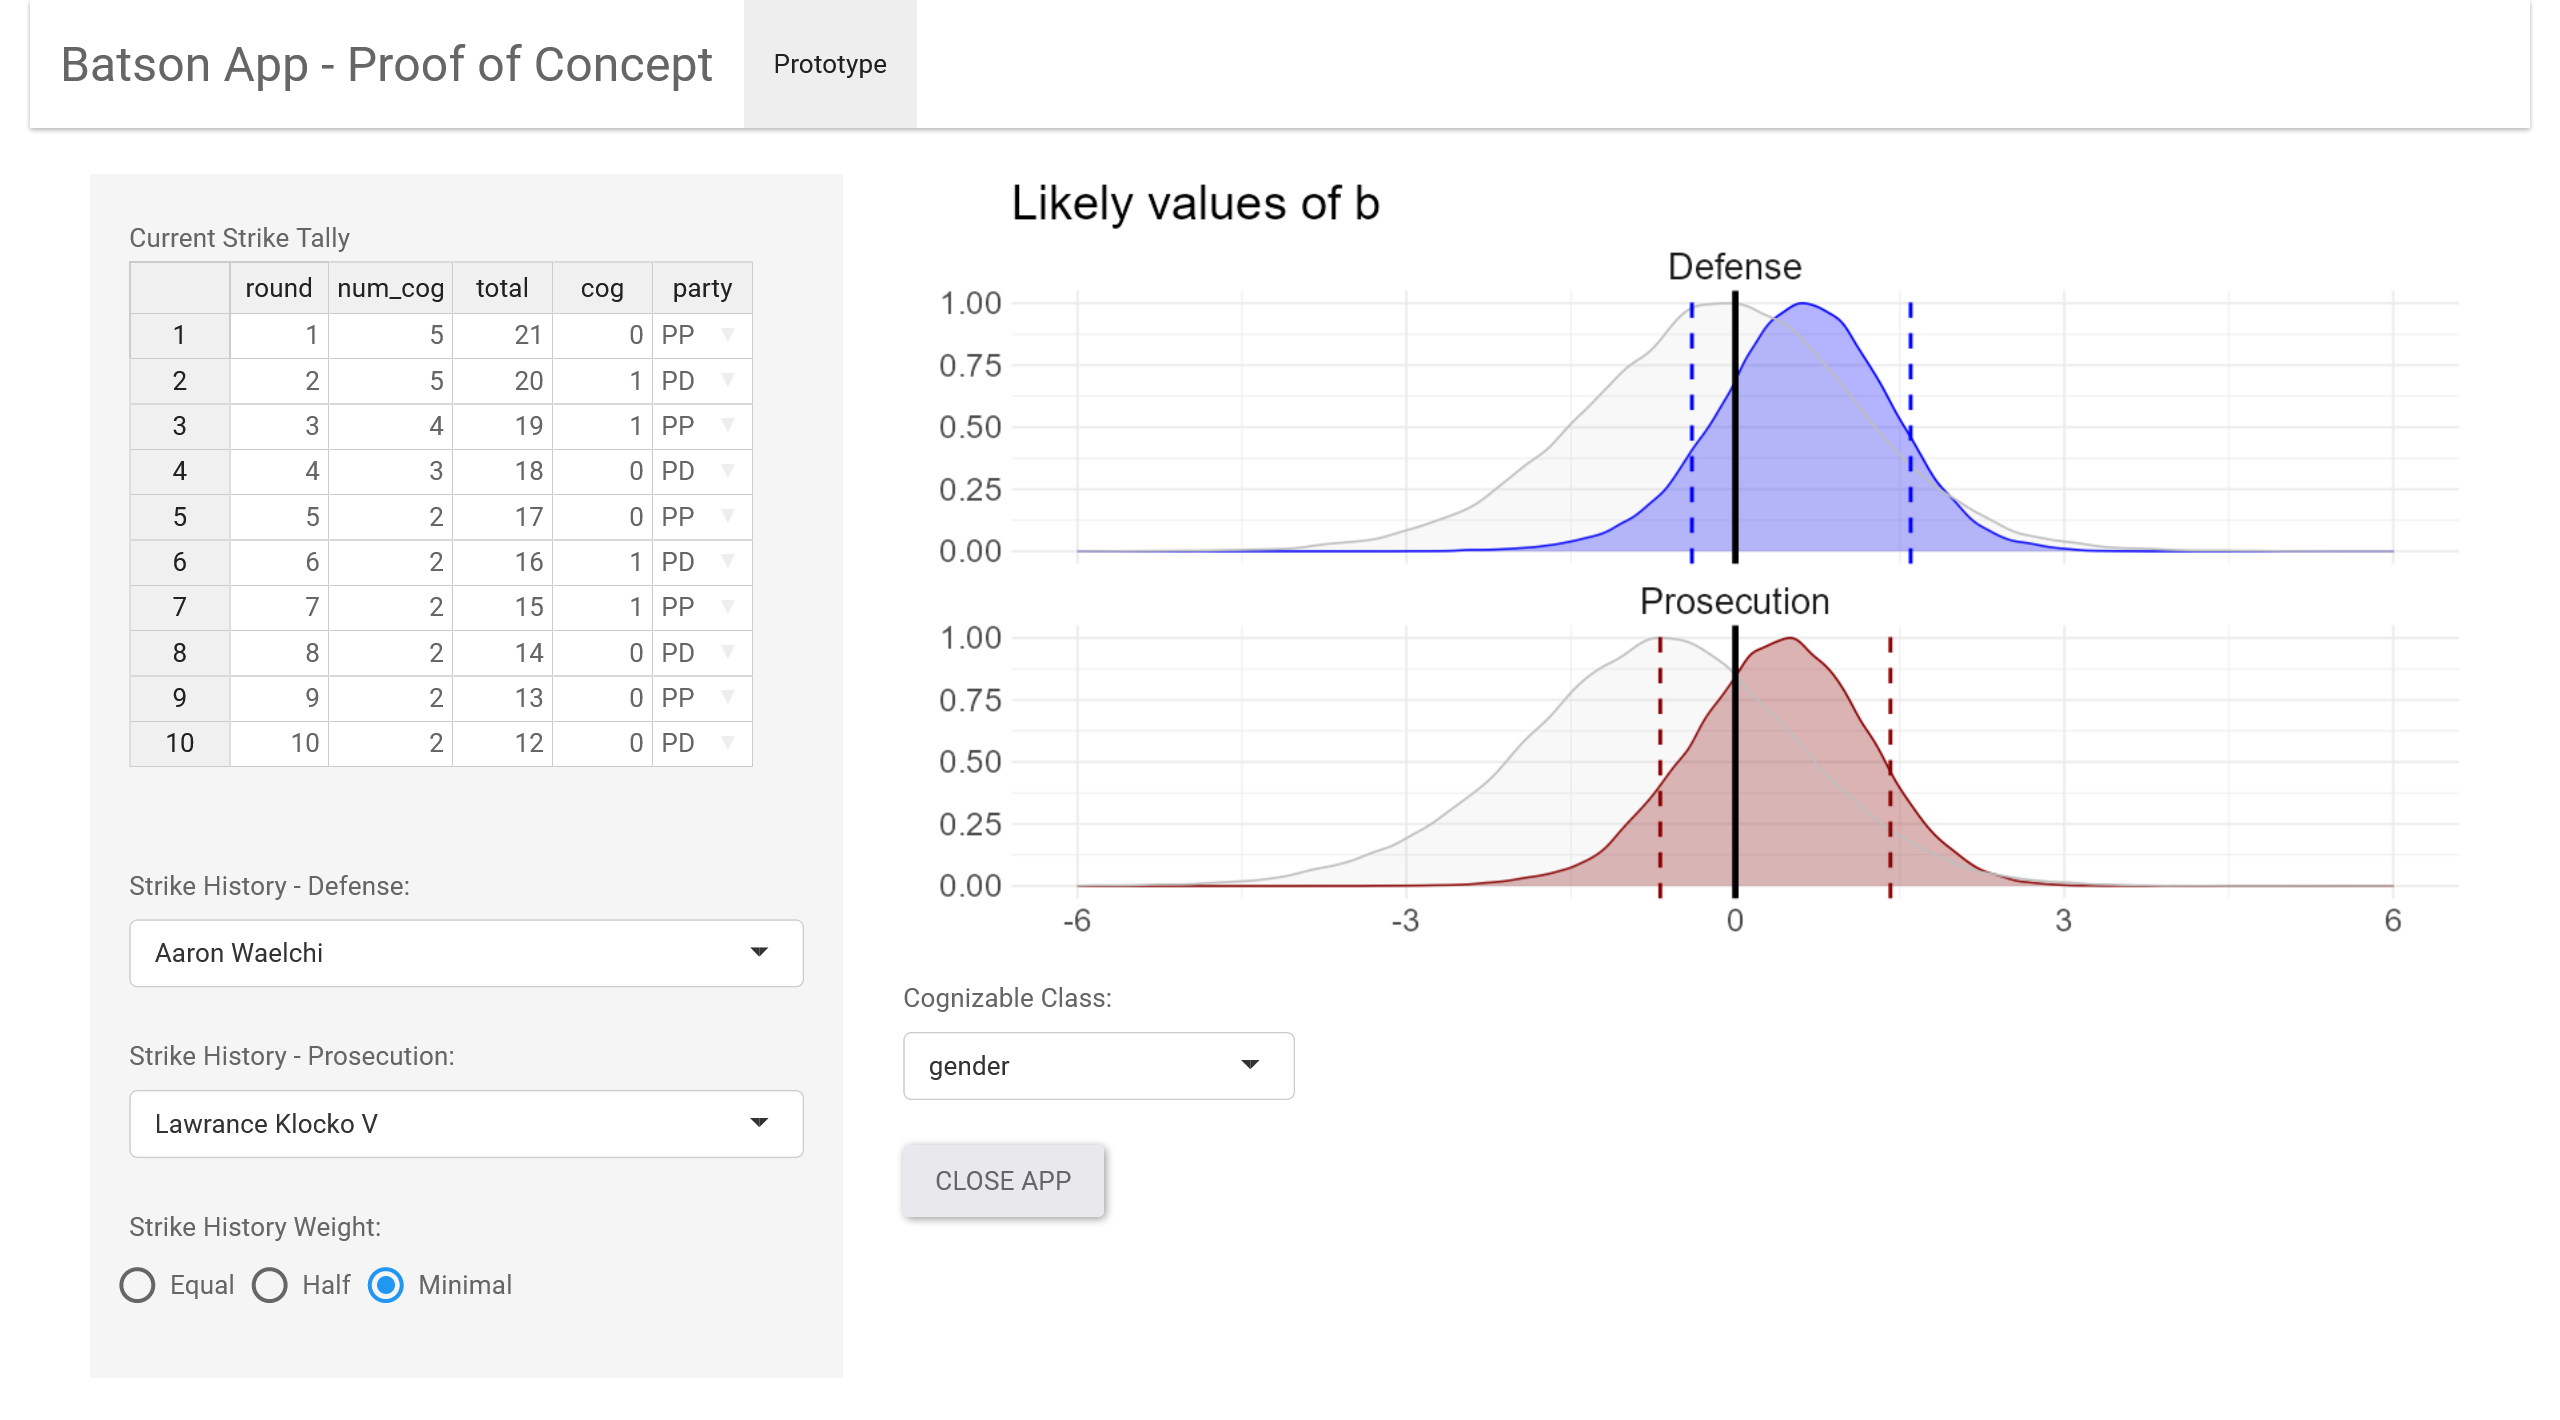
\includegraphics[width=0.5\linewidth]{../figures/batson_app_screenshots/batson_app_screenshot4} \caption{Screenshots of R-Shiny application show density plots for gender bias of prosecutor and defense attorney based on historical and current strike data. Vertical dotted lines depict 95 pct. credible interval.}\label{fig:figapp3}
\end{figure}

Here, most of the prosecutor's density curve of both prior and posterior are to the left of zero, indicating the possible bias against male jurors. However, because the 95\% credible interval includes zero, inferring such bias from the strike data alone is unjustified. Finally, if we assign minimal weight to the historical strike data (\(a = 0.1\)), the density plot updates accordingly (Figure \ref{fig:figapp3}(right)). Both the prior and posterior density become flatter and the credible interval plainly includes zero.



\end{document}
